\documentclass[12pt]{report}
\usepackage{graphicx}
\usepackage{array}
\usepackage{tabularx}
\usepackage{amsmath}
\usepackage{geometry}
\usepackage{fontspec} % For custom font
\usepackage{placeins}
\usepackage{xcolor}
\usepackage{float}
\usepackage{titling}
\usepackage{tikz}
\usepackage{longtable}
\usepackage{fancyhdr} % For custom headers/footers
\usepackage{tocbibind} % To include TOC, LOF, LOT in TOC
\setmainfont{Times New Roman} % Set the main font to Times New Roman
\geometry{a4paper, margin=1in}
\usepackage{setspace}
\onehalfspacing 
\usepackage{titlesec}
\usepackage{fancyhdr}
\usepackage[titles]{tocloft}
\usepackage{chngcnt}
\usepackage{tocbasic}
\PassOptionsToPackage{hyphens}{url}
\usepackage{hyperref}
\usepackage{enumitem}


\newcommand*{\originaltableofcontents}{\listoftoc[\contentsname]{toc}}
\renewcommand*{\listoffigures}{\listoftoc[\listfigurename]{lof}}
\renewcommand*{\listoftables}{\listoftoc[\listtablename]{lot}}
\setuptoc{lof}{totoc}
\setuptoc{lot}{totoc}
\BeforeTOCHead{\clearpage}


\makeatletter
\newcounter{bibitem} % Shared counter for both bibliography and webography
\newenvironment{thebookbibliography}[1]
     {\chapter*{BIBLIOGRAPHIE}
    \addcontentsline{toc}{chapter}{BIBLIOGRAPHIE}    
    \list{\@biblabel{\arabic{bibitem}}}%
           {\usecounter{bibitem}%
            \settowidth\labelwidth{\@biblabel{#1}}%
            \leftmargin\labelwidth
            \advance\leftmargin\labelsep
            \@openbib@code
            \let\p@bibitem\@empty
            \renewcommand\thebibitem{\arabic{bibitem}}}%
      \sloppy
      \clubpenalty4000
      \@clubpenalty \clubpenalty
      \widowpenalty4000%
      \sfcode`\.\@m}
     {\def\@noitemerr
       {\@latex@warning{Empty `thebookbibliography' environment}}%
      \endlist}

\newenvironment{thewebography}[1]
     {\chapter*{WEBOGRAPHIE}
    \addcontentsline{toc}{chapter}{WEBOGRAPHIE}    
    \list{\@biblabel{\arabic{bibitem}}}%
           {\usecounter{bibitem}%
            \settowidth\labelwidth{\@biblabel{#1}}%
            \leftmargin\labelwidth
            \advance\leftmargin\labelsep
            \@openbib@code
            \let\p@bibitem\@empty
            \renewcommand\thebibitem{\arabic{bibitem}}}%
      \sloppy
      \clubpenalty4000
      \@clubpenalty \clubpenalty
      \widowpenalty4000%
      \sfcode`\.\@m}
     {\def\@noitemerr
       {\@latex@warning{Empty `thewebography' environment}}%
      \endlist}
\makeatother




\AfterTOCHead[toc]{\ExecuteDoHook{aftertochead/toc}}

\makeatletter
\newcommand*{\tableofcontentssummary}{%
  \begingroup
    \value{tocdepth}=2\relax% usually show part, chapter and section only
    \@fileswfalse
    \renewcommand*{\contentsname}{SOMMAIRE GENERAL}%
    \setuptoc{toc}{totoc}%
    \originaltableofcontents
  \endgroup
}
\makeatother

\renewcommand*{\tableofcontents}{%
  \renewcommand{\contentsname}{TABLE DES MATIERES}%
  \AddtoOneTimeDoHook{aftertochead/toc}{\maintocsetup}%
  \setuptoc{toc}{totoc}%
  \originaltableofcontents
}
\newcommand*\maintocsetup[1]{%
  \markboth{}{\MakeUppercase{\contentsname}}%
}
\setcounter{tocdepth}{2}


\counterwithout{figure}{chapter}
\counterwithout{table}{chapter}

\renewcommand{\tablename}{Tableau}
\renewcommand{\cftpartpresnum}{PARTIE~} 
\renewcommand{\cftpartaftersnum}{.}     
\renewcommand{\cftpartleader}{\cftdotfill{\cftdotsep}}
\setlength{\cftpartnumwidth}{5em}

\renewcommand{\cftchappresnum}{Chapitre~}
\renewcommand{\cftchapaftersnum}{.}     
\renewcommand{\cftchapleader}{\cftdotfill{\cftdotsep}}
\setlength{\cftchapnumwidth}{5em}

\pagestyle{fancy}
\fancyhf{} % Clear all header and footer fields
\fancyfoot[C]{\thepage} % Place the page number in the center of the footer
\renewcommand{\headrulewidth}{0pt}  % Removes the line in the header
\renewcommand{\footrulewidth}{0pt}  % Removes the line in the footer
\hypersetup{
   colorlinks=true,
  linkcolor=black,   % Set link color to black
  filecolor=magenta, 
  urlcolor=cyan,
  pdfborder={0 0 0} 
}
\renewcommand{\listtablename}{LISTE DES TABLEAUX}
\renewcommand{\listfigurename}{LISTE DES FIGURES}
\newcommand{\figref}[1]{figure \ref{#1}}

\titleformat{\part}[display]
  {\normalfont\Huge\bfseries\centering}
  {PARTIE \Roman{part}}{20pt}{\Huge}

\titleformat{\chapter}[display]
  {\normalfont\Large\bfseries\centering}
  {Chapitre \arabic{chapter}~.}{20pt}{\Large}

\titleformat{\section}
    {\normalfont\large\bfseries} 
    {\thesection}
    {1em}
    {\large}

\titleformat{\subsubsection}
    {\normalfont\Large\bfseries} 
    {\thesubsubsection}
    {1em}
    {\large}
	
\setcounter{secnumdepth}{5}
\renewcommand{\thesubsubsection}{\alph{subsubsection}}
\makeatletter \renewcommand\paragraph{\@startsection{paragraph}{4}{\z@}{3.25ex \@plus1ex \@minus.2ex}{1ex \@plus.2ex}{\normalfont\normalsize\bfseries}} \renewcommand\theparagraph{$\bullet$}
\renewcommand\subparagraph{\@startsection{subparagraph}{5}{\z@}{3.25ex \@plus1ex \@minus.2ex}{1ex \@plus.2ex}{\normalfont\normalsize\bfseries}} \renewcommand\thesubparagraph{$-$} \makeatother

\begin{document}	
			 \pretitle{
				\begin{tikzpicture}[remember picture, overlay]
			   		\node[anchor=north west, xshift=1.5cm, yshift=-1cm] at (current page.north west) {
        						\includegraphics[width=2.5cm]{image1.png}
					};
    					\node[anchor=north west, xshift=4cm, yshift=-1cm] at (current page.north west) {
        						\includegraphics[width=2.3cm]{image2.png}
					};
					\node[anchor=north east, xshift=-1.5cm, yshift=-1cm] at (current page.north east) {
        						
\includegraphics[width=5cm]{image3.png}
					};
				\end{tikzpicture}
				\begin{center}
					\textbf{\large UNIVERSITE DE FIANARANTSOA ECOLE NATIONALE D'INFORMATIQUE \\[0.5cm] MEMOIRE DE FIN D'ETUDES POUR L'OBTENTION DU DIPLOME DE MASTER PROFESSIONNEL}
					\\[0.5cm]
							\textbf{Mention:} Informatique \\	
							\textbf{Parcours:} Informatique générale\\
							\textbf{\textit{Intitulé}}				\end{center}
				\begin{center}\Large\bfseries
			}
			\preauthor{\begin{flushleft}\fontsize{12} \lineskip Présenté le ...\\ }
			\postauthor{\end{flushleft} \textbf{\underline{Membres du Jury:}} 
			 \begin{itemize}
			    \item \textbf{Président:} [président du Jury];
			    \item \textbf{Examinateur:} [examinateur];
			    \item \textbf{Rapporteurs:} \begin{itemize}
       									 \item Monsieur RAZAFIMAHATRATRA Hajarisena, Maître de Conférences;
       									 \item Monsieur RAMILAFANANA Vonjisoa, Ingénieur en Informatique.
    								\end{itemize}
			\end{itemize} }
			\predate{\begin{flushright} Année Universitaire: }
			\postdate{\end{flushright}}
			\title{
				\color{blue}
				\setlength{\fboxsep}{10pt} 
				\begin{center}
					\fbox{
						\begin{minipage}{0.95\textwidth}
							\begin{center}
								CONCEPTION ET REALISATION  D'UNE APPLICATION WEB  DE RESERVATION DE VOYAGE
							\end{center}
						  \end{minipage}
					}
				\end{center}
			}
			\author{Par Monsieur ANDRIAMIORA Ainamalala Lucky}
			\date{2023-2024}
			\maketitle
			
			\newpage
			\thispagestyle{empty}
			\mbox{}

			\newpage
			\pagenumbering{roman}
			\renewcommand{\thepage}{\Roman{page}} % Ensure uppercase Roman numerals
			\setcounter{page}{1}
			\chapter*{CURRICULUM VITAE}
			\addcontentsline{toc}{chapter}{CURRICULUM VITAE}	
			\begin{center}
				\begin{minipage}{0.6\textwidth}
					\textbf{Nom:} ANDRIAMIORA\\
					\textbf{Prenom:} Ainamalala Lucky\\
					\textbf{Numéro:} +261 34 33 513 61\\
					\textbf{Addresse:} IIG20 E Ambatomaro, Antananarivo\\
					\textbf{E-mail:} luckyainamalalalucky@gmail.com\\
					\textbf{Date et lieu de naissance:} 30 décembre 1999 à Antsirabe
				\end{minipage}
				\hfill
				\begin{minipage}{0.3\textwidth}
					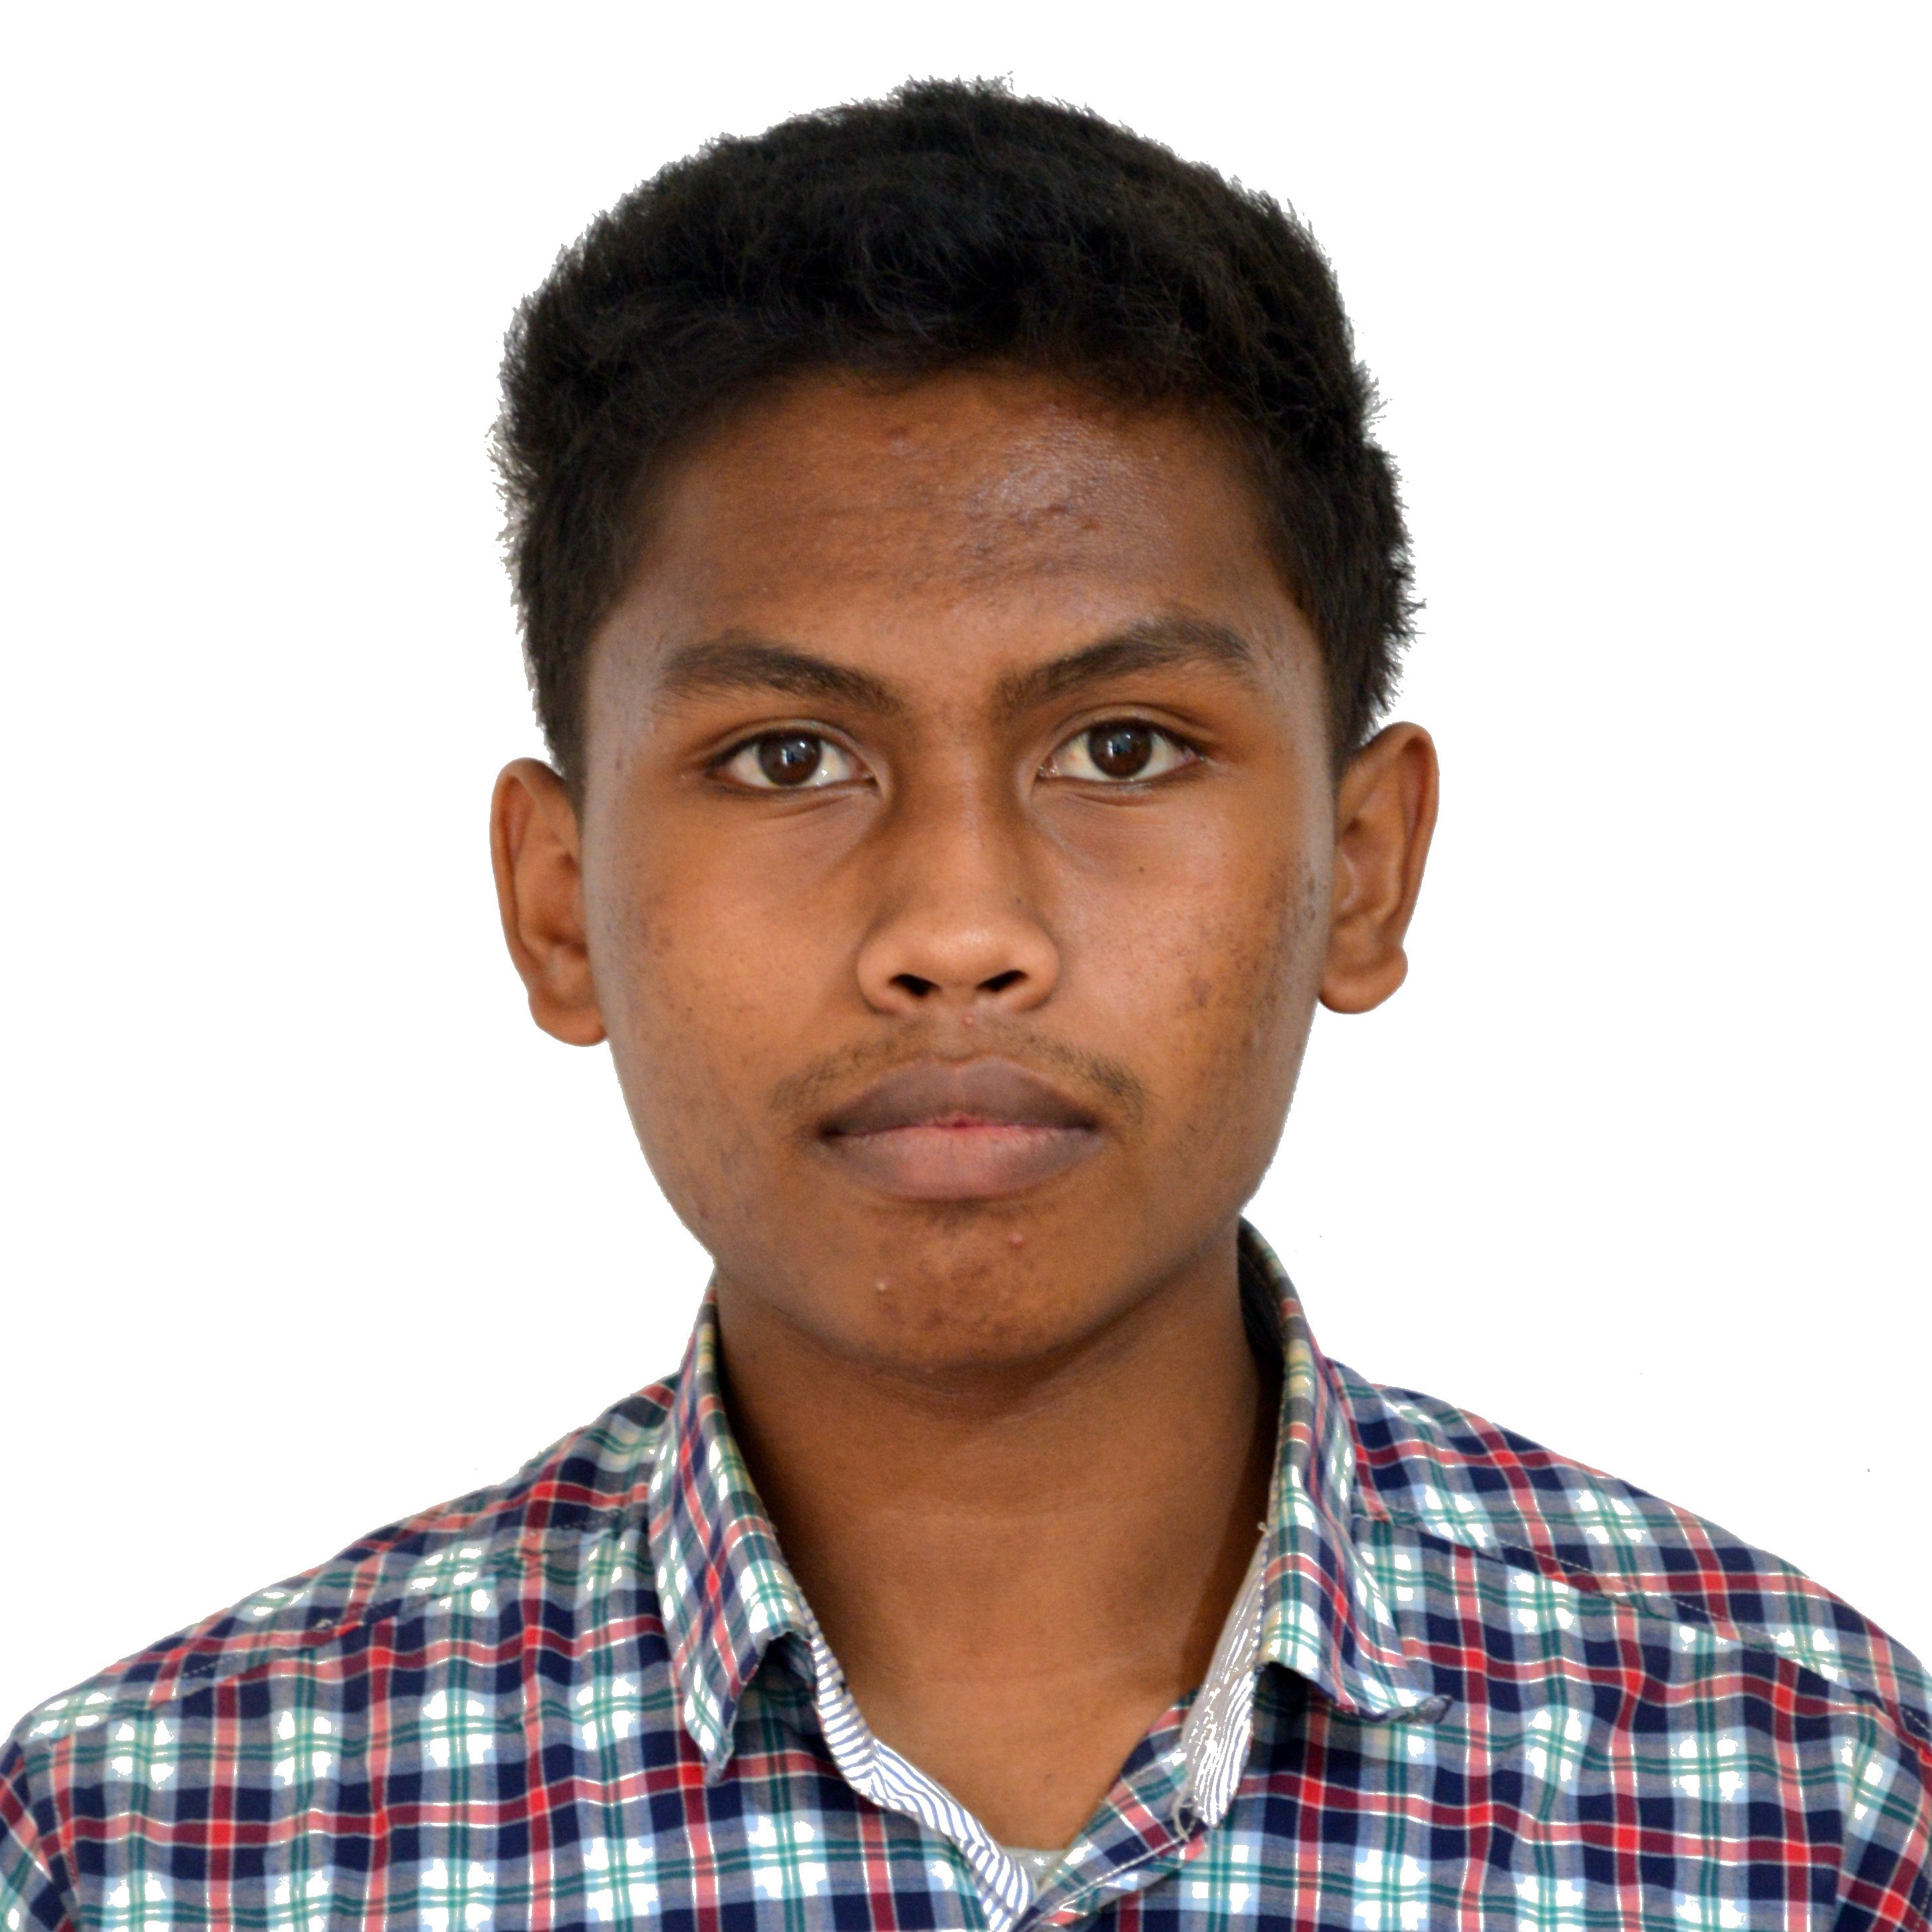
\includegraphics[width=3.5cm, height=3.5cm]{mypic.jpg}	
				\end{minipage}
			\end{center}
			\section*{FORMATIONS ET DIPLOME}
			\begin{center}
				\begin{minipage}{\textwidth}
					\textbf{2024-2025:} Deuxième année de formation en Master professionnelle à l’École Nationale d'Informatique, Université de Fianarantsoa, parcours : Informatique générale.\\[0.5cm]
					\textbf{2023-2024:} Première année de formation en Master professionnelle à l’École Nationale d'Informatique, Université de Fianarantsoa, parcours : Informatique générale.\\[0.5cm]
					\textbf{2022-2023:} Obtention du diplôme de Licence professionnelle mention Bien à l’École Nationale d'Informatique, Université de Fianarantsoa, parcours : Informatique générale.\\[0.5cm]
					\textbf{2021-2022:} Deuxième année de formation en Licence professionnelle à l’École Nationale d'Informatique, Université de Fianarantsoa, parcours : Informatique générale.\\[0.5cm]
					\textbf{2020-2021:} Première année de formation en Licence professionnelle à l’École Nationale d'Informatique, Université de Fianarantsoa, parcours : Informatique générale.\\[0.5cm]
					\textbf{2019-2020:} Obtention du diplôme de Baccalauréat série D mention assez-bien au Lycée André Résampa Antsirabe.
				\end{minipage}
			\end{center}
			\section*{STAGES ET EXPERIENCES PROFESSIONNELLES}
			\begin{center}
				\begin{minipage}{\textwidth}
       					 \textbf{11 juin 2024 au 4 novembre 2024:} Stage auprès de Nexitia technologies.
						\begin{itemize}
							\item Thème du stage: Application web Handeha voyage;
							\item Langages et outils: Java, spring boot, JavaScript, next js, Katappult, H2, UML.						
						\end{itemize}
       					 \textbf{Octobre 2023:} Projet à l’École Nationale d'Informatique.
						\begin{itemize}
							\item Thème du stage: Module de securité pour application spring boot et angular;
							\item Langages et outils: Java, spring boot, Angular, TypeScript, PostgreSQL, UML.						
						\end{itemize}       					 
					\textbf{19 octobre 2022 au 16 janvier 2023:} Stage auprès de la Paositra malagasy.
						\begin{itemize}
							\item Thème du stage: Application web pour la gestion des change;
							\item Langages et outils: Java, spring boot, Angular, TypeScript, PostgreSQL, UML.								
						\end{itemize}
					\textbf{Septembre 2022:} Projet à l’École Nationale d'Informatique.
						\begin{itemize}
							\item Thème du stage: Création d'une application mobile de gestion de cotisation de groupe;
							\item Langages et outils: Java, Android Studio.								
						\end{itemize}
					\textbf{8 mars 2021 au 7 juillet 2021:} Stage auprès du Ministère de l’Économie et de la Finance.
						\begin{itemize}
							\item Thème du stage: Application web pour la gestion des dossier du personnels de la Direction du Système d'Information;
							\item Langages et outils: Java, spring boot, Angular, TypeScript, PostgreSQL, UML.								
						\end{itemize} 
					\textbf{Avril 2021:} Projet à l’École Nationale d'Informatique.
						\begin{itemize}
							\item Thème du stage: Réalisation d’une application desktop de Gestion des heures complémentaires;
							\item Langages et outils: Php, MySQL, Ajax.								
						\end{itemize} 
					\textbf{Août 2020:} Projet à l’École Nationale d'Informatique.
						\begin{itemize}
							\item Thème du stage: Création d'une application desktop de gestion de stock;
							\item Langages et outils: C++, Qt Creator.								
						\end{itemize} 
   				\end{minipage}		
			\end{center}
			\section*{CONNAISSANCES EN INFORMATIQUE}
			\begin{center}
				\begin{minipage}{\textwidth}
					\begin{center}
						\begin{tabularx}{\textwidth}{|X|X|}
							\hline
							\textbf{Systèmes d'exploitation:} & Microsoft Windows, Linux\\
							\hline
							\textbf{Langages de Programmation:} & Java, JavaScript, TypeScript, Python , C/C++\\
							\hline
							\textbf{Technologies de développements:} &  React.js, Next.js, Angular, Express.js, Spring Framework, J2EE\\
							\hline
							\textbf{Technologies Web:} & HTML5, CSS3\\
							\hline
							\textbf{API:} & REST\\
							\hline
							\textbf{Compétences en bases de données:} &  SQL, PostgreSQL, MySQL\\
							\hline
							\textbf{Outils de Gestion de Versions:} & Git, GitHub, GitLab\\
							\hline
							\textbf{Outils DevOps:} &  Docker, Kubernetes, Jenkins, Ansible\\
							\hline
							\textbf{Outils de virtualisation:} & Docker, VirtualBox, VMware, Vagrant\\
							\hline
							\textbf{Outils de tests et Assurance Qualité:} & Jest, JUnit\\
							\hline
							\textbf{Méthodes de conception:} &2TUP, MERISE\\
							\hline
							\textbf{Méthode de gestion de projet:} &Méthode AGILE - SCRUM\\
							\hline
							\textbf{Langage de modélisation:} & UML\\
							\hline
							\textbf{Outil de gestion de projet:} & Trello\\
							\hline
						\end{tabularx}
					\end{center}
	   			\end{minipage}		
			\end{center}
			\section*{CONNAISSANCES LINGUISTIQUE}
			\begin{center}
				\begin{minipage}{\textwidth}
					\begin{center}
						\begin{tabularx}{\textwidth}{|X|X|X|X|X|}
							\hline
							\textbf{Langues} & \textbf{Comprehension} & \textbf{Lecture} & \textbf{Parler} & \textbf{Ecrire}\\
							\hline
							Anglais & Bien & Bien & Assez-bien & Bien \\
							\hline
							Français & Bien & Bien & Bien & Bien\\
							\hline
						\end{tabularx}
					\end{center}
				\end{minipage}
			\end{center}
			\section*{LOISIR ET CENTRES D'INTERET}
			\begin{center}
				\begin{minipage}{\textwidth}
					\begin{itemize}
						\item Musique;
						\item Podcast;
						\item Documentaires;
						\item Anime;
						\item Jeux video;
						\item	Lecture.
					\end{itemize}
				\end{minipage}	
			\end{center}
	






			\newpage
				\tableofcontentssummary
			\newpage








			\chapter*{REMERCIEMENTS}
			\addcontentsline{toc}{chapter}{REMERCIEMENTS}	
					\hspace{15pt} Avant toute chose, je tiens à remercier Dieu tout puissant et miséricordieux, qui m'a donné la force et la patience d'accomplir ce modeste travail.

					Mes remerciements s’étendent également à :

					\begin{itemize}
						\item Monsieur \textbf{HAJALALAINA Aimé Richard}, Professeur et Président de l’Université de Fianarantsoa, pour le bon déroulement de l’année universitaire.;
						\item Monsieur \textbf{MAHATODY Thomas}, Professeur, Directeur de l’École Nationale d'Informatique, qui nous à donné l'opportunité d'aller en stage pour ainsi permettre d’accroître nos compétences;
						\item Monsieur \textbf{RAMILAFANANANA Vonjisoa}, CEO de NEXITIA TECHNOLOGIES et mon encadreur professionnel, pour son accueil et la confiance qu'il à accordée depuis mon arrivée dans l’établissement;
						\item Monsieur \textbf{RABETAFIKA Louis Haja}, Maître de Conférences et Responsable de Mention, pour ses conseils durant notre formation;
						\item Monsieur \textbf{GILANTE Gesazafy}, Assistant d'Enseignement Supérieur et de recherche et responsable du parcours Informatique Générale, pour sa pédagogie inspirante;
						\item Monsieur \textbf{RAZAFIMAHATRATRA Hajarisena}, Maître de Conférences à l’Université de Fianarantsoa et responsable du Parcours « Objets Connectés et Cybersécurité », qui a bien voulu assurer l’encadrement de l’élaboration de ce mémoire et de nous avoir honoré par sa présence au jury en tant qu’encadreur;
					 	\item Monsieur [président du jury], Maître de Conférences à l’Université de Fianarantsoa, pour sa disponibilité et d’avoir bien voulu accepter de présider le Jury;
						\item Monsieur [examinateur], [titre], Examinateur qui a bien voulu prendre le temps de valoriser et d'évaluer ce travail de mémoire. 
					\end{itemize}

						Enfin un grand remerciement à tous les enseignants et les personnels administratifs au sein de l’Ecole Nationale d’Informatique mais surtout à ma famille qui m’ont épaulé aussi bien moralement que financièrement et sans oublier mes amis, mes anciens collègues qui par biais des échanges ont élargis ma perspective et ont renforcés ma compréhension de ce sujet.

			\newpage
			\listoftables
			\newpage
			\listoffigures
			\newpage
			\chapter*{NOMENCLATURE}
			\addcontentsline{toc}{chapter}{NOMENCLATURE}


			\begin{longtable}{|p{4cm}|p{10cm}|} 
			\hline
				\textbf{API} & Application Programming Interface\\
			\hline
				\textbf{ACID} & Atomicity, Consistency, Isolation, Durability\\
			\hline
				\textbf{ASR} & Administration des Systèmes et Réseaux\\
			\hline
				\textbf{CNH} & Commission Nationale d’Habilitation\\
			\hline
				\textbf{CPU} & Central Processing Unit\\
			\hline
				\textbf{CUR} & Centre Universitaire Régional\\
			\hline
				\textbf{ERD} & Entity Relashionship Diagram\\
			\hline
				\textbf{GB} & Génie logiciel et Base de Données\\
			\hline
				\textbf{GID} & Gouvernance et Ingénierie de Données\\
			\hline
				\textbf{HTML} & HyperText Markup Language\\
			\hline
				\textbf{HTTP} & HyperText Transfer Protocol\\
			\hline
				\textbf{HTTPS} & HyperText Transfer Protocol Secure\\
			\hline
				\textbf{IA} & Intelligence Artificielle\\
			\hline
				\textbf{IBM} & International Business Machines\\
			\hline
				\textbf{IDE} & Integrated Development Environment\\
			\hline
				\textbf{IG} & Informatique Générale\\
			\hline
				\textbf{JDK} & Java Development Kit\\
			\hline
				\textbf{JSON} & JavaScript Object Notation\\
			\hline
				\textbf{JSF} & JavaServer Faces\\
			\hline
				\textbf{JVM} & Java Virtual Machine\\
			\hline
				\textbf{LMD} & Licence – Master - Doctorat\\
			\hline
				\textbf{MVVM} & Model-View-ViewModel\\
			\hline
				\textbf{OCC} & Objets connectés et Cybersécurité\\
			\hline
				\textbf{ORM} & Object-Relational Mapping\\
			\hline
				\textbf{OMG} & Object Management Group\\
			\hline
				\textbf{RAM} & Random Access Memory\\
			\hline
				\textbf{RG} & Règle de Géstion\\
			\hline
				\textbf{SGBD} & Système de Gestion de Base de Données\\
			\hline
				\textbf{SGBDR} & Système de Gestion de Base de Données Relationnelles\\
			\hline
				\textbf{SQL} & Structured Query Language\\
			\hline
				\textbf{SSD} & Solid-State Drive\\
			\hline
				\textbf{SVN} & Subversion\\
			\hline
				\textbf{SSII} & Société de Services en Ingénierie Informatique\\
			\hline
				\textbf{TIC} & Technologies de l’Information et de la Communication\\
			\hline
				\textbf{UML} & Unified Modeling Language\\
			\hline
				\textbf{URL} & Uniform Resource Locator\\
			\hline
				\textbf{VCS} & Version Control System\\
			\hline
				\textbf{XML} & eXtensible Markup Language\\
			\hline
				\textbf{XP} & extreme Programming\\
			\hline
			\end{longtable}

			\newpage
			\pagenumbering{arabic}
			\setcounter{page}{1}
			\chapter*{INTRODUCTION GÉNÉRALE}
			\addcontentsline{toc}{chapter}{INTRODUCTION GÉNÉRALE}
			\begin{center}
				\begin{minipage}{\textwidth}
					\hspace{15pt} Avec sa biodiversité unique et sa richesse culturelle, Madagascar est une destination touristique de choix. Cependant, avec la demande pour des expériences de voyage personnalisées et accessibles en ligne en constante croissance, de nombreux opérateurs touristiques luttent pour obtenir la visibilité et les moyens nécessaires pour promouvoir efficacement leurs offres.\\
	
					\hspace{15pt} Malgré l'essor des plateformes de réservation en ligne, il demeure un besoin urgent d'une solution centralisée pour permettre aux opérateurs touristiques malgaches de partager leurs offres et aux voyageurs de réserver facilement leurs circuits ou séjours.\\
	
					\hspace{15pt} L'objectif de ce mémoire est de développer et de présenter "Handeha Voyage", une application web qui  facilite la mise en ligne des offres de circuits et de séjours par les opérateurs touristiques, simplifie le processus de réservation pour les utilisateurs et améliore la visibilité des opérateurs touristiques. Cette étude propose une solution novatrice qui répond directement aux défis rencontrés par les opérateurs touristiques et les voyageurs à Madagascar. En effet, l'application "Handeha Voyage" ne se contente pas de faciliter la réservation des voyages; elle redéfinit fondamentalement la manière dont les services touristiques sont présentés et consommés.\\
	
					\hspace{15pt} Ce mémoire abordera le processus de conception, de développement et de mise en œuvre de l'application "Handeha Voyage". Nous utiliserons des méthodes de conception et de modélisation adaptées, ainsi que des langages de programmation et frameworks appropriés, sans oublier un système de gestion de base de données solide. Tout cela sera orchestré selon une méthodologie de gestion de projet bien définie pour assurer une organisation optimale. Les limitations incluent le temps limité pour le développement complet de certaines fonctionnalités avancées, l'accès limité aux données et la difficulté à recueillir des retours d'expérience durant le développement.\\
	
					\hspace{15pt} Notre plan se subdivise en trois parties: dans un premier temps la présentation de l’École Nationale d'Informatique (ENI) suivie de celle de Nexitia Technology. Dans la deuxième partie, nous aborderons les analyses et la conception du projet. Enfin, la troisième partie portera sur la réalisation du projet avec les différents moyens et outils utilisés.
				\end{minipage}
			\end{center}
			\part{PRESENTATION}
			\chapter{Présentation de l’Ecole Nationale d’Informatique}

			\hspace{15pt} Ce chapitre offre un aperçu détaillé de l'Ecole Nationale d’Informatique, mettant en lumière son rôle essentiel dans la formation des professionnels de l'informatique à Madagascar, ses missions, son histoire et son impact sur le développement technologique du pays.			

			\section{Information d’ordre générale }
				\hspace{15pt} L’Ecole Nationale d’Informatique, en abrégé ENI, est un établissement d’enseignement supérieur rattaché académiquement et administrativement à l’Université de Fianarantsoa. Le siège de l’Ecole se trouve à Tanambao-Antaninarenina à Fianarantsoa. L’adresse pour la prise de contact avec l’Ecole est la suivante : Ecole Nationale d’Informatique (ENI) Tanambao, Fianarantsoa. Le numéro de sa boîte postale est 1487 avec le code postal 301. Téléphone : 034 05 733 36 ou 032 15 204 28. Son adresse électronique est la suivante : eni@eni.mg. Il dispose également d'un site web : \textbf{www.eni.mg}.

			\section{Missions et historiques}
				\hspace{15pt} L’ENI se positionne sur l’échiquier socio-éducatif malgache comme étant le plus puissant secteur de diffusion et de vulgarisation des connaissances et des technologies informatiques. 

				Cette Ecole Supérieure peut être considérée aujourd’hui comme la vitrine et la pépinière des élites informaticiennes du pays.
	
				De façon formelle, l’ENI était créée par le décret N° 83- 185 du 24 Mai 1983, comme étant le seul établissement Universitaire Professionnalisé au niveau national, destiné à former des techniciens et des Ingénieurs de haut niveau, aptes à répondre aux besoins et exigences d’Informatisation des entreprises, des sociétés et des organes implantés à Madagascar.

				L’ENI a pour conséquent pour mission de former des spécialistes informaticiens compétents et opérationnels de différents niveaux notamment: 
				
								\begin{itemize}
									\item En fournissant à des étudiants des connaissances de base en informatique;
									\item En leur transmettant le savoir-faire requis, à travers la professionnalisation des formations dispensées et en essayant une meilleure adéquation des formations par rapport aux besoins évolutifs des sociétés et des entreprises;
									\item En initiant les étudiants aux activités de recherche dans les différents domaines des Technologies de l’Information et de la Communication (TIC).
								\end{itemize}

				La filière de formation d’Analystes Programmeurs a été mise en place à l’Ecole en 1983, et a été gelée par la suite en 1996, tandis que la filière de formation d’ingénieurs a été ouverte à l’Ecole en 1986.
				
				Une formation de troisième cycle a été ouverte à l’Ecole a été ouverte à l’Ecole depuis l’année 2003 – 2004 grâce à la coopération académique et scientifique entre l’Université de Fianarantsoa pour le compte de l’ENI et l’Université Paul Sabatier de Toulouse (UPST).

				Cette filière avait pour objectif de former certains étudiants à la recherche dans les différents domaines de l’Informatique, et notamment pour préparer la relève des Enseignants-Chercheurs qui étaient en poste.

				Pendant l’année 2007-2008, la formation en vue de l’obtention du diplôme de Licence Professionnelle en Informatique a été mise en place à l’ENI avec les deux parcours de formation:
					
						\begin{itemize}
							\item Génie Logiciel et base de Données;
							\item Administration des Système et réseaux.
						\end{itemize}
				
				La mise en place à l’Ecole de ces deux options de formation devait répondre au besoin de basculement vers le système Licence – Master – Doctorat (LMD). 
En vue de surmonter les difficultés de limitation de l’effectif des étudiants accueillis à l’Ecole, notamment à cause du manque d’infrastructures, un système de « Formation Hybride » a été mise en place à partir de l’année 2010. Il s’agit en effet d’un système de formation semi présentielle et à distance avec l’utilisation de la visioconférence pour la formation à distance. Le système de formation hybride a été ainsi créé à Fianarantsoa ainsi qu’Université de Toliara. Cette formation est à l’origine du parcours Informatique Générale.

				En 2023, une nouvelle mention Intelligence Artificielle (IA) a été ouvert au sein de l’Ecole pour répondre les besoins des entreprises. La formation est destinée aux étudiants titulaires du diplôme de licence (Bac +3) en Mathématiques ou en Statistiques ou en Informatique, etc. La mention IA comporte deux parcours:

						\begin{itemize}
							\item Gouvernance et Ingénierie de Données (GID);
							\item Objets connectés et Cybersécurité (OCC).
						\end{itemize}

				Le principe de l’enseignement pour le parcours GID offre aux l’étudiants des compétences scientifiques et techniques spécialisées en Science de données. Pour le parcours OCC, les étudiants octroient la double spécialité premièrement en internet des objets et deuxièmement en cybersécurité. La formation de master est axée sur l’ensemble d’applications de l’Intelligence Artificielle.

				\section{Organigramme institutionnel}

				\hspace{15pt} L’organigramme de l’Ecole est inspiré des dispositions du décret N° 83-185 du 24 Mai 1983. L’ENI est administrée par un Conseil d’Ecole, et dirigée par un directeur nommé par un décret adopté en Conseil des Ministres. Le Collège des enseignants regroupant tous les enseignants-chercheurs permanents de l’Ecole est chargé de résoudre les problèmes liés à l’organisation pédagogique des enseignements. Le Conseil Scientifique propose les orientations pédagogiques et scientifiques de l’établissement, en tenant compte notamment de l’évolution du marché de travail et de l’adéquation des formations dispensées par rapport aux besoins des entreprises. 

				La figure \ref{fig:OrganigrammeENI} représente l’organigramme actuel de l’ENI.

				\begin{figure}[h]
					\centering
					\includegraphics[width=\textwidth]{image4.png}
					\caption{Organigramme actuel de l’Ecole}
					\label{fig:OrganigrammeENI}
				\end{figure}
				\clearpage
				
				\section{Domaine de spécialisation}
				\hspace{15pt} Les activités de formation et de recherche organisées à l’ENI portent sur les domaines suivants: 

						\begin{itemize}
							\item Génie logiciel et Base de Données ;
							\item Administration des Systèmes et Réseaux ;
							\item Informatique Générale ;
							\item Modélisation informatique et mathématique des Systèmes complexes.
							\item Intelligence artificielle
						\end{itemize}

				Le tableau \ref{tab:formationPedagogiqueENI} décrit l’organisation du système de formation pédagogique de l’Ecole.

				\begin{table}[h]
				  \centering
				  \caption{Organisation du système de formation pédagogique de l’Ecole}
				  \label{tab:formationPedagogiqueENI}
					  \begin{tabular}{|p{7cm}|p{7cm}|}
					    \hline
					    \textbf{Formation Théorique} & \textbf{Formation Pratique} \\
					    \hline
					    \begin{itemize}
						\item Enseignement théorique
						\item Travaux dirigés
						\item Travaux pratiques
						\item Conférences
					    \end{itemize}
					 &  
					\begin{itemize}
						\item Etude de cas
						\item Travaux de réalisation
						\item Projets/ Projets tutoriels
						\item Voyages d’Etudes
						\item Stages en entreprise
					\end{itemize}
					\\
					    \hline
					  \end{tabular}
				\end{table}

				\section{Architecture des formations pédagogiques}

				\hspace{15pt} Le recrutement des étudiants à l’ENI se fait uniquement par voie de concours d’envergure nationale en première année. Les offres de formation organisées à l’Ecole ont été validées par la Commission Nationale d’Habilitation (CNH). Au sein de l’ENI, il existe deux mentions et cinq parcours.

				Le tableau \ref{tab:mentionsEtParcoursENI} récapitule les mentions et les parcours au sein de l’Ecole.

				\begin{table}[h]
				  \centering
				  \caption{Mention et parcours au sein de l’ENI}
				  \label{tab:mentionsEtParcoursENI}
					  \begin{tabular}{|p{7cm}|p{7cm}|}
						\hline 
						\textbf{Mention} & \textbf{Parcours} \\
						\hline 
						\textbf{Informatique} & Génie logiciel et Base de Données (GB) \\ \cline{2-2} & Administration des Systèmes et Réseaux (ASR) \\ \cline{2-2} & Informatique Générale (IG) \\ 
						\hline 
						\textbf{Intelligence Artificielle} & Gouvernance et Ingénierie de Données (GID) \\ \cline{2-2} & Objets Connectés et Cyber sécurités (OCC) \\
						\hline 
					  \end{tabular}
				\end{table}
				\FloatBarrier

				La figure \ref{fig:LMD} représente l’architecture des études correspondant au système LMD.

				\begin{figure}[h]
					\centering
					\includegraphics[width=\textwidth]{image5.png}
					\caption{Architecture des études correspondant au système LMD}
					\label{fig:LMD}
				\end{figure}
				\FloatBarrier
				
				La licence peut avoir une vocation générale ou professionnelle. Le master peut avoir une vocation professionnelle ou de recherche. L’accès en première année de MASTER se fait automatiquement pour les étudiants de l’Ecole qui ont obtenu le diplôme de Licence Professionnelle.				

				Le tableau \ref{tab:formationsENI} illustre la liste des formations existantes à l’ENI.

				\begin{table}[h]
				  \centering
				  \caption{Liste des formations existantes à l’ENI}
				  \label{tab:formationsENI}
				 \resizebox{\textwidth}{!}{
					  \begin{tabular}{|p{4cm}|p{5cm}|p{5cm}|}
						 \hline
						  & \multicolumn{2}{|c|}{\textbf{Formation}} \\
						 \hline
						  &  \textbf{Licence Professionnelle} & \textbf{master} \\
						 \hline
						 \textbf{Condition admission} &
						Par voie de concours
 						 &  Par voie de concours pour la mention IA\\
						 \hline
					 	\textbf{Condition d’Accès} & Bac de série C, D ou Technique& Être titulaire de licence professionnelle\\					
						\hline
						\textbf{Durée de Formation} & 3 ans & 2 ans\\
						\hline
						\textbf{Diplôme délivré} & Diplôme de Licence Professionnelle &
						\begin{itemize}
							\item Diplôme de Master Professionnel;
							\item Diplôme de Master Recherche.
						\end{itemize}\\
						\hline
					  \end{tabular}
				}
				\end{table}
				\FloatBarrier				

				Le Master Recherche permet à son titulaire de poursuivre directement des études en doctorat et de s’inscrire directement dans une Ecole Doctorale.

				Les étudiants diplômés de l’Ecole sont plutôt bien accueillis dans les instituts universitaires étrangères (Canada, Suisse, France, …).

				\section{Relation de l’ENI avec les organismes externes}
				
				\hspace{15pt} Les stages effectués chaque année par les étudiants mettent l’Ecole en rapport permanent avec plus de 400 entreprises et organismes publics, semi-publics et privés, nationaux et internationaux. L’Ecole dispose ainsi d’un réseau d’entreprises, de sociétés et d’organismes publics et privés qui sont des partenaires par l’accueil en stage de ses étudiants, et éventuellement pour le recrutement après l’obtention des diplômes par ces derniers. Les compétences que l’Ecole cherche à développer chez ses étudiants sont l’adaptabilité, le sens de la responsabilité, du travail en équipe, le goût de l’expérimentation et l’innovation.

				En effet, la vocation de l’ENI est de former des licenciés et des ingénieurs de niveau MASTER avec des qualités scientifiques, techniques et humaines reconnues, capables d’évoluer professionnellement dans des secteurs d’activité variés intégrant l’informatique. Les stages en milieu professionnel permettent de favoriser une meilleure adéquation entre les formations à l’Ecole et les besoins évolutifs du marché de l’emploi.

				Parmi les sociétés, les entreprises et les organismes partenaires de l’Ecole, on peut citer : ACCENTURE Mauritius, AKATA Goavana, Air Madagascar, Ambre Associates, Airtel, Agence Universitaire de la Francophonie (AUF), AXIAN, B2B, Banque Centrale, , BIANCO, BlueLine, CNaPS, Bureau National de Gestion des Risques et des Catastrophes (BNGRC), CEDII-Fianarantsoa, Data Consulting, Central Test, Centre National Antiacridien, CNRE, COLAS, Direction Générale des Douanes, DLC, E-Tech Consulting, , FID, FIHARY Soft, FTM, GNOSYS, GENIUS AT WORK, Hello Tana, IBONIA, INGENOSIA, INSTAT, IOGA, JIRAMA, JOUVE, MADADEV, MAEP, MANAO, MEF, MEN, MESupRES, MFB, , MININTER, Min des Postes/Télécommunications et du Développement Numérique, NEOV MAD, Ny Havana, Madagascar National Parks, OMNITEC, ORANGE, OTME, PRACCESS, QMM Fort-Dauphin, SG Madagasikara SMMC, SMMEC, SNEDADRS Antsirabe, Sénat, Société d’Exploitation du Port de Toamasina (SEPT), SOFTWELL, Strategy Consulting, TELMA, VIVETEC, Société LAZAN’I BETSILEO, WWF, UGD, ARATO, MANAO, MNDPT, NG ACADEMY.NG, Relia … 			
				
				\section{Débouchés professionnels et diplômés}

				\hspace{15pt} Les formations proposées par l’Ecole permettent aux diplômés d’être immédiatement opérationnels sur le marché du travail avec la connaissance d’un métier complet lié à l’informatique aux TIC.

				L’Ecole apporte à ses étudiants un savoir-faire et un savoir-être qui les accompagnent tout au long de leur vie professionnelle. Elle a une vocation professionnalisante. Les diplômés en LICENCE et en MASTER issus de l’ENI peuvent faire carrière dans différents secteurs. 

				L’Ecole bénéficie aujourd’hui de 40 années d’expériences pédagogiques et de reconnaissance auprès des sociétés, des entreprises et des organismes. C’est une Ecole Supérieure de référence en matière informatique.

				D’une manière générale, les diplômés de l’ENI n’éprouvent pas de difficultés particulières à être recrutés au terme de leurs études. Cependant, l’ENI recommande à ses diplômés de promouvoir l’entrepreneuriat en TIC et de créer des cybercafés, des SSII ou des bureaux d’études. 

				Le tableau \ref{tab:debouchesENI} représente les débouchés éventuels des jeunes diplômés.

				\begin{table}[h]
				  \centering
				  \caption{Débouchés éventuels des jeunes diplômés}
				  \label{tab:debouchesENI}
				  \resizebox{\textwidth}{!}{
				    \begin{tabular}{|p{5cm}|p{10cm}|}
				      \hline
				      LICENCE & 
				      \begin{itemize}
				        \item Analyste – Programmeur ;
				        \item Administrateur de site web/de portail web;
				        \item Assistant Informatique et internet;
				        \item Chef de projet web ou multimédia;
				        \item Développeur Informatique ou multimédia;
				        \item Intégrateur web ou web designer;
				        \item Hot liner/Hébergeur Internet;
				        \item Agent de référencement;
				        \item Responsable de sécurité web;
				        \item Technicien/Supérieur de help desk sur Informatique;
				        \item Administrateur de réseau.
				      \end{itemize} \\
				      \hline
				     MASTER & 
				      \begin{itemize}
				        \item Administrateur de réseau et système;
				        \item Architecture de système d’information;
				        \item Développeur d’applications;
				        \item Ingénieur réseau;
				        \item Webmaster / Web Designer;
				        \item Concepteur et réalisateur d’application;
				        \item Directeur du système d’informations;
				        \item Chef de projet informatique;
				        \item Responsable de sécurité informatique;
				        \item Consultant fonctionnel ou freelance.
				      \end{itemize} \\
				      \hline
				    \end{tabular}
				  }
				\end{table}
				\clearpage

				\section{Ressources humaines}

				\hspace{15pt} Les ressources humaines sont citées ci-dessous selon leurs responsabilités :

				\begin{itemize}
					\item Directeur de l’Ecole : Monsieur MAHATODY Thomas, Professeur ;
					\item Responsable de la Mention « Informatique » : Monsieur RABETAFIKA Louis Haja, Maître de Conférences ;
					\item Responsable de la Mention « Intelligence Artificielle » : Monsieur DIMBISOA William Germain, Maître de Conférences ;
					\item Responsable du Parcours « Génie Logiciel et Base de Données » : Monsieur RALAIVAO Jean Christian, Maître de Conférences ;
					\item Responsable du Parcours « Administration Systèmes et Réseaux » : Monsieur SIAKA, Assistant d’Enseignement Supérieur et de Recherche ;
					\item Responsable du Parcours « Informatique Générale » : Monsieur GILANTE Gesazafy, Assistant d’Enseignement Supérieur et de Recherche ;
					\item Responsable du Parcours « Gouvernance et Ingénierie de Données » : Madame RATIANANTITRA Volatiana Marielle, Maître de Conférences ;
					\item Responsable du Parcours « Objets Connectés et Cybersécurité » : Monsieur RAZAFIMAHATRATRA Hajarisena, Maître de Conférences.
				\end{itemize}

				L’ENI compte quinze (15) enseignants permanents dont un (01) Professeur Titulaire, un (01) Professeur, un (01) Docteur HDR, huit (08) Maîtres de Conférences, quatre (04) Assistants d’Enseignement Supérieur et de Recherche, dix (10) enseignants vacataires, quarante un (41) personnel administratif.





				\chapter{Présentation de Nexitia Technologies}

				\hspace{15pt} Dans ce chapitre, nous allons parler de NEXITIA Technologies. C'est une entreprise innovante, bien connue pour ses solutions technologiques avancées. Nous verrons son histoire, ses débuts, ainsi que sa vision et sa mission. Nous mettrons également en avant les partenariats stratégiques qui augmentent son influence dans le domaine du développement d'applications.

				\section{Information générale sur la société}

				\hspace{15pt} Nexitia Technologies est une startup dynamique et innovante, fondée par Vonjisoa RAMILAFANANANA, un pionnier de l'industrie du développement de logiciels. Fort d'une expérience de plus de 15 ans en tant qu'ingénieur en informatique, Monsieur RAMILAFANANANA incarne la vision novatrice de l'entreprise.

				Nexitia Technologies se distingue par son engagement à fournir des solutions qui répondent aux défis actuels des entreprises, tout en promouvant l'innovation et la créativité dans le secteur numérique. L'expertise de son fondateur et son engagement envers l'avancement technologique sont au cœur de la mission de l'entreprise, visant à transformer la manière dont les applications sont développées et utilisées.

				\section{Historique et Origines}

				\hspace{15pt} Nexitia Technologies a été fondée par Vonjisoa RAMILAFANANANA, en 2020, un ingénieur en informatique reconnu pour son expérience auprès de clients prestigieux tels qu'Airbus, Thales, Total Energies et Channel. Animée par une vision audacieuse, l'entreprise vise à révolutionner le processus de développement d'applications. Grâce à ses années d'expérience, Monsieur RAMILAFANANANA a identifié un besoin criant sur le marché : la nécessité d'une solution de développement de logiciels plus rapide, efficace et accessible. Cette observation a donné naissance à Katappult, qui a évolué d'une simple idée en une plateforme low code complète.

				Aujourd'hui, l'enthousiasme est palpable chez Nexitia Technologies, alors que l'entreprise se prépare à lancer Katappult sur le marché. Avec l'ambition de devenir un partenaire clé pour les entreprises en quête de solutions innovantes, Nexitia Technologies s'efforce de répondre aux besoins des entrepreneurs qui cherchent à accélérer et optimiser leur processus de développement de logiciels. L'entreprise cherche également à établir des partenariats stratégiques pour élargir sa portée et maximiser son impact, consolidant ainsi sa position dans l'écosystème technologique en pleine évolution.

				\section{Vision et Mission}

				\hspace{15pt} La vision de Nexitia Technologies est de transformer le paysage numérique en rendant le développement d'applications accessible à tous, quel que soit leur niveau de compétence technique. L’entreprise aspire à démocratiser l’innovation en fournissant des outils qui permettent aux utilisateurs de créer et de gérer des solutions numériques sans les barrières traditionnelles du codage.				

				La mission de Nexitia Technologies est de fournir des solutions performantes et flexibles via sa plateforme Katappult. En offrant une approche low-code, Nexitia vise à simplifier le processus de développement tout en permettant aux entreprises d'accélérer leur transformation numérique. L'entreprise s'engage à répondre aux besoins spécifiques de ses clients en leur fournissant des applications sur mesure qui optimisent leur efficacité opérationnelle.

				En parallèle, Nexitia Technologies se positionne comme un partenaire stratégique pour ses clients, les accompagnant dans chaque étape de leur projet, de la conception à la mise en œuvre. Grâce à une approche centrée sur le client et à un engagement envers l'innovation continue, Nexitia s'efforce de créer des solutions qui non seulement répondent aux défis actuels, mais anticipent également les besoins futurs du marché.

				\section{NEXITIA et ses partenaires}

				\hspace{15pt} Nexitia a récemment annoncé un partenariat stratégique avec IONOS, un fournisseur de services d'hébergement cloud. Cette collaboration vise à améliorer le déploiement d'applications web et mobiles en fournissant une infrastructure optimisée et des solutions adaptées aux développeurs.

				\subsection{Objectifs du Partenariat}

				Le partenariat entre Nexitia et IONOS a plusieurs objectifs clés :

				\begin{itemize}
					\item \textbf{Facilitation du Développement:} En offrant des outils et des ressources adaptés, Nexitia souhaite simplifier le processus de création d'applications mobiles pour les développeurs ;
					\item \textbf{Optimisation des Performances:} L'infrastructure cloud d'IONOS permettra d'améliorer la vitesse et la fiabilité des applications, garantissant une meilleure expérience utilisateur ;
					\item \textbf{Support Technique:} Les développeurs bénéficieront d'un soutien technique accru pour les aider à surmonter les défis liés au déploiement et à la gestion de leurs applications.
				\end{itemize}

				 \subsection{Impact sur le Marché}

				Cette initiative pourrait avoir un impact significatif sur le marché des applications mobiles :

				\begin{itemize}
					\item \textbf{Attraction de Nouveaux Développeurs:} En rendant le développement d'applications plus accessible, Nexitia et IONOS pourraient attirer un plus grand nombre de développeurs et d'entreprises souhaitant innover dans ce domaine ;
					\item \textbf{Amélioration de l'Expérience Utilisateur:} Avec des applications plus performantes et fiables, les utilisateurs finaux bénéficieront d'une expérience améliorée, ce qui pourrait accroître l'adoption des nouvelles technologies.
				\end{itemize}





				\chapter{Description du projet}

				\hspace{15pt} Ce chapitre présente une description détaillée du projet "Handeha Voyage", en couvrant sa nature, ses objectifs, les besoins des utilisateurs, les moyens nécessaires à sa réalisation et les résultats attendus.

				\section{Formulation}
				
				\hspace{15pt} Madagascar, avec sa biodiversité unique et sa richesse culturelle, est une destination touristique de choix. Cependant, de nombreux opérateurs touristiques rencontrent des difficultés pour obtenir la visibilité et les moyens nécessaires afin de promouvoir efficacement leurs offres. Le projet "Handeha Voyage" vise à développer une plateforme web centralisée, permettant aux opérateurs de mettre en ligne leurs offres de circuits et de séjours, et aux voyageurs de réserver facilement leurs voyages.
	
				\section{Objectifs et besoins des utilisateurs}

						\hspace{15pt} Les objectifs principaux de l'application "Handeha Voyage" sont les suivants :
						\begin{itemize}
							\item Amélioration de la visibilité: Augmenter la visibilité des opérateurs touristiques malgaches sur le marché numérique;
							\item Facilitation des réservations : Simplifier le processus de réservation pour les utilisateurs;
							\item Optimisation de la gestion : Fournir aux opérateurs des outils efficaces pour gérer leurs offres et leurs réservations.
						\end{itemize}

						L'application répondra donc aux besoins suivants de chaque utilisateur:

						\begin{itemize}
							\item Opérateurs touristiques :
								\begin{itemize}
									\item Interface utilisateur intuitive pour mettre à jour leurs offres;
									\item Outils de gestion des réservations et des paiements;
									\item Accès à des statistiques et analyses pour optimiser leurs offres.
								\end{itemize}		
							\item Voyageurs:
								\begin{itemize}
									\item Rechercher et réserver des offres de circuits et de séjours de manière simplifiée;
									\item Consulter les avis et évaluations pour aider dans la prise de décision;
									\item Sécurité des paiements et des informations personnelles.
								\end{itemize}
						\end{itemize}

						L'application devra aussi répondre aux critères suivants:

						\begin{itemize}
							\item \textbf{Extensibilité :}  L'application doit être extensible pour permettre l'ajout de nouvelles fonctionnalités à l'avenir;
							\item \textbf{Convivialité :} L'interface doit être simple et facile à manipuler, même pour les utilisateurs novices;
							\item \textbf{Performance :} L'application doit être rapide et capable de gérer un grand nombre de requêtes simultanées;
							\item \textbf{Sécurité :} L'application doit garantir la confidentialité et l'intégrité des données personnelles des utilisateurs.
						\end{itemize}
								
				\section{Moyens nécessaires à la réalisation du projet}

				\hspace{15pt} Pour mener à bien ce projet, il est essentiel de disposer des ressources adéquates. Dans cette section, nous détaillerons les différents moyens nécessaires à la réalisation du projet, qu'ils soient humains, matériels ou logiciels.

				\subsection{Moyens Humains}

				\hspace{15pt} Cette section présente les différents profils professionnels et les équipes nécessaires à la réalisation des objectifs du projet.				

				Le Tableau \ref{tab:moyensHumains} représente les moyens humains nécessaires à la réalisation du projet.

				\begin{table}[h]
				  \centering
				  \caption{Inventaire des moyens humains}
				  \label{tab:moyensHumains}
				  \resizebox{\textwidth}{!}{
				    \begin{tabular}{|p{5cm}|p{3cm}|p{6cm}|}
					      \hline
					      \textbf{Fonction} & \textbf{Nombre} & \textbf{Rôle}\\
					      \hline
					      Maître d’ouvrage & 	1  & Le Product Owner\\
					     \hline
					     Chef de projet & 1 & Ingénieur en Informatique : Scrum Master\\
						\hline
 						Développeurs & 4 & 
						\begin{itemize}
							\item Un ingénieurs en informatique;
							\item Deux étudiant en dernière année de master en informatique;
							\item Un étudiant en dernière année de licence en informatique.
						\end{itemize}\\						

						\hline
						Designer UX/UI & 1 &\\
						\hline
						Testeur & 1 & Ingénieur en Informatique\\
						\hline
						Professionnels du tourisme et de l'hôtellerie & 3 &
						\begin{itemize}
							\item Un diplômé en tourisme et hôtellerie;
							\item Deux stagiaires en tourisme et hôtellerie.
						\end{itemize}\\
 						\hline 
				    \end{tabular}
				  }
				\end{table}
				\FloatBarrier

				\subsection{Moyens matériels}

				\hspace{15pt} Cette section présente les différents moyens matériels nécessaires, allant des équipements informatiques aux logiciels et autres ressources techniques indispensables pour atteindre les objectifs fixés.

				Le tableau \ref{tab:moyensMateriels} représente l’ensemble des matériels utilisés lors de la mise en œuvre de l’application :

				\begin{table}[h]
				  \centering
				  \caption{Inventaire des moyens matériels}
				  \label{tab:moyensMateriels}
				  \resizebox{\textwidth}{!}{
				    \begin{tabular}{|c|p{5cm}|c|c|}
					      \hline
						     \textbf{Désignation} & \textbf{Caractéristiques} & \textbf{Quantité} & \textbf{Utilité}\\
					      \hline
							Ordinateur portable &
							\begin{itemize}
								\item \textbf{Processeur:} Intel core i5-1135G7 @ 2.40GHz(8 CPUs), ~ 2.4GHz;
								\item \textbf{RAM:} 16Go;
								\item \textbf{Disque dur:} 500Go.
							\end{itemize}
							& 4 & Développement et tests\\
						\hline
							Ordinateur portable &
							\begin{itemize}
								\item \textbf{Processeur:} Intel Core i7 2.5GHz;
								\item \textbf{RAM:} 16Go;
								\item \textbf{Disque dur:} 512Go.
							\end{itemize}
							& 1 & Développement et tests\\
						\hline

				    \end{tabular}
				  }
				\end{table}
				\FloatBarrier

				\subsection{Moyens Logiciels}

				\hspace{15pt} Cette section détaille les divers logiciels nécessaires pour le développement, la gestion et l'exécution efficace des différentes tâches liées au projet.

				Le Tableau \ref{tab:moyensLogiciels} représente les logiciels nécessaires au développement et à la mise en œuvre de "Handeha Voyage".

				\begin{table}[h]
				  \centering
				  \caption{Inventaire des moyens logiciels}
				  \label{tab:moyensLogiciels}
				    \begin{tabular}{|p{4cm}|p{3cm}|p{7cm}|}
					      \hline
					      \textbf{Désignation} & \textbf{Version} & \textbf{Utilité}\\
					      \hline
					      Visual Studio Code & 1.93.1 & Éditeur de code\\
					     \hline
					     Eclipse & 2024-06 & Environnement de développement intégré (IDE)\\
						\hline
 						PostgreSQL & 16.1 & Gestion de la base de données\\
						\hline
						Visual Paradigm & 16.1 & Outils de modélisation et de conception\\
						\hline
						Git & - & Gestion des versions et collaboration\\
						\hline
						Trello & - & Gestion de projet et organisation des tâches\\
						\hline
						Google Chrome & 130.0.6723.127 & Navigateur web pour tester la plateforme\\
						\hline
						Postman & 11.17 & Outil permettant de tester les API et simuler des requêtes HTTP\\
						\hline
						Katappult & Beta Version & Plateforme de développement low-code\\
						\hline 
				    \end{tabular}
				\end{table}
				\FloatBarrier


				\subsection{Résultats Attendus}

				\hspace{15pt} Les résultats attendus de ce projet incluent :
				
				\begin{itemize}
					\item Une augmentation de la visibilité des opérateurs touristiques malgaches;
					\item Une simplification du processus de réservation pour les utilisateurs;
					\item Une application sécurisée, fiable et facile à utiliser, répondant aux besoins des utilisateurs;
					\item Une amélioration continue basée sur les retours d'expérience des utilisateurs.
				\end{itemize}

				\subsection{Chronogramme d'activités}

				\hspace{15pt} Afin de planifier et de suivre efficacement l'avancement du projet, il est essentiel d'établir un chronogramme détaillé des activités. Cette section présente le calendrier des principales étapes et tâches, en précisant les délais.

				 La Figure \ref{fig:Chronogramme} représente le diagramme de gant du chronogramme d'activités du projet.

				\begin{figure}[h]
					\centering
					\includegraphics[width=\textwidth]{image6.png}
					\caption{Diagramme de gant du chronogramme d'activités du projet}
					\label{fig:Chronogramme}
				\end{figure}
				\FloatBarrier







				\part{ANALYSE ET CONCEPTION}
				\chapter{Analyse préalable}
				
				\hspace{15pt}L'analyse préalable est une étape cruciale dans la préparation de tout projet. Elle consiste à examiner et à comprendre les besoins, les contraintes et les opportunités avant de lancer le développement.

				 Nous allons voir, dans ce chapitre, l’analyse de l’existant, les critiques de l’existant et la conception avant-projet.

				\section{Analyse de l'existant}
				
				\hspace{15pt} Pour élaborer une solution numérique efficace, il est crucial d'analyser en profondeur le système actuel. Cette analyse nous permettra de comprendre les forces et les faiblesses du système existant, afin de proposer des améliorations pertinentes.

				\subsection{Organisation actuelle}
				
				\hspace{15pt} Le secteur touristique malgache repose actuellement sur une diversité de plateformes pour la promotion des offres touristiques. Chaque opérateur utilise des outils variés, tels que des sites web individuels, des pages sur les réseaux sociaux, et des systèmes de gestion des réservations distincts. 

				En plus de ces méthodes, certains opérateurs se tournent vers des marketplaces globales comme Booking.com ou TripAdvisor pour atteindre un public international.

				 Cette approche fragmentée mène à une faible visibilité des offres touristiques locales, une complexité accrue dans la gestion des réservations, et des inefficacités opérationnelles.

				En l'absence d'une plateforme intégrée, les opérateurs doivent naviguer entre plusieurs outils, ce qui peut entraîner des redondances et des erreurs. De plus, les voyageurs rencontrent des difficultés pour comparer les offres et réserver leurs voyages de manière fluide, ce qui impacte leur expérience globale.

				\subsection{Moyens matériels et logiciels}
				\hspace{15pt} Le tableau \ref{tab:materielsLogicielsOrganisationAct} représente les moyens matériels et logiciels nécessaires à l'organisation actuelle.
				\begin{table}[h]
				  \centering
				  \caption{Moyens matériels et logiciels de l'organisation actuelle}
				  \label{tab:materielsLogicielsOrganisationAct}
				  \resizebox{\textwidth}{!}{
				    \begin{tabular}{{|p{7.5cm}|p{7.5cm}|}}
					      \hline
						    \textbf{Moyens matériels} & \textbf{Moyens logiciels}\\
					      \hline
							\begin{itemize}
								\item Ordinateurs
								\item Smartphones/Tablettes
								\item Serveurs
								\item Connexions Internet
								\item Imprimantes/Scanners
								\item Caméras numériques
							\end{itemize} & 
							\begin{itemize}
								\item Sites Web
								\item Réseaux Sociaux
								\item Google Sheets
								\item Logiciels de gestion interne	
								\item Plateformes de réservation
							\end{itemize}\\
						\hline

				    \end{tabular}
				  }
				\end{table}
				\FloatBarrier				

				\section{Critique de l'existant}

				\hspace{15pt} L'analyse du système actuel de gestion des offres touristiques à Madagascar révèle plusieurs aspects positifs et défis majeurs.
				
				Le tableau \ref{tab:tableau 8} représente les points forts et les points faibles de l'organisation actuelle.
		
				\begin{table}[h]
				  \centering
				  \caption{Critique de l'organisation actuelle.}
				  \label{tab:tableau 8}
				  \resizebox{\textwidth}{!}{
				    \begin{tabular}{|p{7.5cm}|p{7.5cm}|}
					      \hline
						     \textbf{Points forts} & \textbf{Points faibles}\\
					      \hline
							\begin{itemize}
								\item \textbf{Présence en Ligne:} Les opérateurs touristiques ont commencé à établir leur présence en ligne grâce à des sites web et des pages sur les réseaux sociaux, ce qui permet de toucher un public large et diversifié.
								\item \textbf{Accès à une Audience Internationale:} L'utilisation de plateformes comme Booking.com et TripAdvisor offre aux opérateurs une visibilité auprès d'un public international.
								\item \textbf{Communication Directe avec les Clients:} Les réseaux sociaux et les applications de messagerie comme WhatsApp et Messenger facilitent une communication rapide et directe avec les clients, ce qui est un avantage pour la gestion des demandes de renseignements et des réservations.
							\end{itemize} & 
							\begin{itemize}
								\item \textbf{Fragmentation des Plateformes:} La diversité des plateformes et des outils crée une fragmentation qui complique la gestion des réservations et des informations. : Les mises à jour des offres et des disponibilités ne sont pas synchronisées entre les différentes plateformes. Chaque opérateur utilise des systèmes différents, ce qui entraîne des redondances et des risques d'erreurs.
								\item \textbf{Coûts Élevés:} Les commissions élevées imposées par les marketplaces globales réduisent les marges bénéficiaires des opérateurs locaux, rendant difficile la compétitivité sur le marché international.
								\item \textbf{Expérience Utilisateur Fragmentée:} Les clients doivent naviguer entre plusieurs plateformes pour trouver des informations et effectuer des réservations, ce qui peut être frustrant et décourageant. L'absence d'une solution intégrée nuit à l'expérience utilisateur.
								\item \textbf{Adaptabilité Locale Insuffisante:} Les solutions actuelles, bien qu'utilisées, ne prennent pas en compte les spécificités culturelles et opérationnelles du marché malgache, limitant leur efficacité.
							\end{itemize}\\
						\hline

				    \end{tabular}
				  }
				\end{table}
				\FloatBarrier				

				\section{Conception avant projet}
				
				\hspace{15pt} Les opérateurs touristiques à Madagascar rencontrent des difficultés majeures dans la gestion et la promotion de leurs offres en raison de la fragmentation des outils et des plateformes utilisés. Actuellement, chaque opérateur utilise une variété de sites web, réseaux sociaux et systèmes de gestion des réservations, ce qui entraîne des inefficacités et des incohérences.

				\subsection{Proposition de solutions}

				\hspace{15pt} Pour développer et optimiser les activités touristiques à Madagascar, les solutions suivantes ont été proposées, visant à renforcer la compétitivité et à maximiser les opportunités de croissance pour les opérateurs touristiques:

				\begin{itemize}
					\item \textbf{Solution1:} Créer une plateforme numérique centralisée dédiée à la promotion des offres touristiques et à la gestion des réservations.
					\item \textbf{Solution2:} Créer une agence de marketing numérique spécialisée dans le secteur touristique malgache.
				\end{itemize}

				Le tableau \ref{tab:solutions} représente les avantages et les inconvénients des deux solutions.

				\begin{table}[h]
				  \centering
				  \caption{Avantages et inconvénients des solutions proposées.}
				  \label{tab:solutions}
				  \resizebox{\textwidth}{!}{
				    \begin{tabular}{|p{5cm}|p{5cm}|p{5cm}|}
					      \hline
						     \textbf{Solution}  & \textbf{Avantages}  & \textbf{Inconvénients} \\
					      \hline
						\textbf{Solution1:}  Créer une plateforme numérique centralisée dédiée à la promotion des offres touristiques et à la gestion des réservations. &
						\begin{itemize}
							\item Augmentation de la visibilité des offres touristiques locales.
							\item Amélioration de l'efficacité opérationnelle grâce à une gestion centralisée.
							\item Réduction des coûts de gestion et des commissions des plateformes globales.
							\item Optimisation de l'expérience utilisateur pour les clients.
						\end{itemize}
						&
						\begin{itemize}
							\item Coûts de développement et de maintenance élevés.
							\item Besoin de formation des opérateurs pour l'adoption et l'utilisation efficace de la plateforme.
							\item Risques liés à la cybersécurité et à la protection des données sensibles.
							\item Dépendance à une infrastructure technologique stable et performante.
						\end{itemize}\\						
						\hline
						\textbf{Solution2:}  Créer une agence de marketing numérique spécialisée dans le secteur touristique malgache. &
						\begin{itemize}
							\item Offre une expertise spécialisée en marketing numérique adapté au secteur touristique.
							\item Augmente la visibilité des opérateurs touristiques sur le web et les réseaux sociaux.
							\item Permet aux opérateurs de se concentrer sur leur cœur de métier tout en déléguant le marketing à des experts.
							\item Création de campagnes publicitaires ciblées pour atteindre une audience spécifique et augmenter les réservations.
						\end{itemize}
						&
						\begin{itemize}
							\item Coûts initiaux pour établir et développer l'agence.
							\item Nécessité de recruter et de former du personnel qualifié en marketing numérique.
							\item Dépendance à l'efficacité des stratégies de marketing pour générer des résultats tangibles.
							\item Risques de fluctuation des demandes et des tendances du marché.
						\end{itemize}\\						

						\hline
				    \end{tabular}
				  }
				\end{table}
				\clearpage
				\subsection{Solution retenue}

				\hspace{15pt} Pour résoudre les difficultés majeures rencontrées par les opérateurs touristiques à Madagascar dans la gestion et la promotion de leurs offres, la solution suivante a été retenue. Développer une application web centralisée, "Handeha Voyage", qui regroupe les offres touristiques de Madagascar. Cette plateforme permet aux opérateurs de mettre en ligne leurs circuits et séjours de manière cohérente et efficace.

				Cette solution simplifie le processus de réservation pour les voyageurs, améliore la visibilité des opérateurs et optimise la gestion des offres touristiques en réduisant les inefficacités dues à la fragmentation des outils actuels.

				Vu les avantages cités, la solution retenue est donc de développer "Handeha Voyage" pour centraliser les offres touristiques, améliorer la gestion et la promotion des opérateurs locaux, et simplifier le processus de réservation pour les voyageurs.

				\subsection{Méthodes de conception et outils utilisés}
				\subsubsection{Méthode de conduite de projet}

				\hspace{15pt} Le développement d'une application inclut inévitablement une phase de conception cruciale. Cette étape garantit que l'application atteindra les objectifs fixés tout en assurant la fiabilité des résultats et la robustesse de l'application. Elle doit respecter les contraintes de qualité, de coûts et de détails. La phase de conception facilite également le dialogue entre les concepteurs, les développeurs et les utilisateurs, servant de référence tout au long du développement et de la maintenance.
	
				Commençons tout d'abord par voir les différentes méthodes que nous avons à disposition.

				Le tableau \ref{tab:agileVStrad} recense les principaux points forts et points faibles des approches traditionnelles et les méthodes agiles.

				\begin{longtable}{|p{3cm}|p{5.5cm}|p{5.5cm}|} 
						\caption{Comparaison entre les différentes méthodes possibles pour la gestion de projet\cite{Doc4Dev}.} 
						\label{tab:agileVStrad}\\ 
						\hline 
						\textbf{Méthodes} & \textbf{Avantages} & \textbf{Inconvénients}\\ 
						\hline 
						\endfirsthead 	
						\caption[]{(Suite)}\\ 
						\hline 
						\textbf{Méthodes} & \textbf{Avantages} & \textbf{Inconvénients}\\ 
						\hline 
						\endhead
						En cascade &
						\begin{itemize}
							\item \textbf{Structure claire:} Chaque phase doit être complétée avant de passer à la suivante, ce qui offre une approche structurée et séquentielle.
							\item \textbf{Documentation détaillée:} La méthode en cascade met fortement l'accent sur la documentation à chaque étape.
							\item \textbf{Facilité de gestion:} La nature séquentielle de la méthode facilite la planification et la gestion des projets.
						\end{itemize} &
						\begin{itemize}
							\item \textbf{Inflexibilité:} Difficile de revenir en arrière ou d'apporter des modifications une fois qu'une phase est terminée.
							\item \textbf{Risque accru:} Si les erreurs ne sont détectées qu'en fin de cycle, elles peuvent être coûteuses à corriger.
							\item \textbf{Temps de développement long:} Peut ralentir le processus de développement car chaque phase doit être complètement terminée avant de passer à la suivante.
						\end{itemize}\\
						\hline 
						Cycle en V &
						\begin{itemize}
							\item \textbf{Validation et vérification:} Chaque phase de développement est directement associée à une phase de test correspondante, assurant une qualité élevée.
							\item \textbf{Documentation complète:} Comme la méthode en cascade, le cycle en V met un fort accent sur la documentation.
							\item \textbf{Détection précoce des défauts:} Les tests sont planifiés dès le début, ce qui permet de détecter et de corriger les défauts plus tôt.
						\end{itemize} &
						\begin{itemize}
							\item \textbf{Rigidité:} Comme la méthode en cascade, il est difficile d'apporter des modifications en cours de route.
							\item \textbf{Coût élevé des modifications:} Les changements sont coûteux et difficiles à intégrer une fois le processus lancé.
							\item \textbf{Non adapté aux projets flexibles:} Pas idéal pour les projets où les exigences peuvent évoluer au fil du temps.
						\end{itemize}\\
						\hline 
						Méthode Agile &
						\begin{itemize}
							\item \textbf{Flexibilité:} Agile permet des ajustements rapides en fonction des retours des utilisateurs ou des changements du marché.
							\item \textbf{Livraisons fréquentes:} Les itérations courtes conduisent à des livraisons fréquentes de fonctionnalités utilisables.
							\item \textbf{Collaboration accrue:} Encourage une communication constante entre les équipes et les parties prenantes.
							\item \textbf{Réduction des risques:} Les revues régulières et les ajustements fréquents réduisent les risques de grands échecs de projet.
							\item \textbf{Satisfaction client:} Les clients voient régulièrement des progrès et peuvent influencer la direction du projet.
						\end{itemize} &
						\begin{itemize}
							\item \textbf{Manque de documentation:} La priorité sur le développement rapide peut mener à une documentation insuffisante.
							\item \textbf{Difficulté de mise à l'échelle:} Les grands projets peuvent avoir du mal à adopter Agile sans une gestion rigoureuse.
							\item \textbf{Nécessite une forte implication:} Requiert une implication constante et active des parties prenantes.
						\end{itemize}\\
						\hline 
				    \end{longtable}

				\paragraph{Choix du méthode}

				Nous avons choisi la méthodologie Agile pour le developpement de "Handeha Voyage" en raison de sa fléxibilité face aux nombreux changements du projet.
				
				Agile permet une adaptation rapide aux retours constants sur les besoins, garantissant ainsi un produit final de haute qualité.				

				\paragraph{Présentation de la méthode agile}

				La méthodologie Agile est un cadre de gestion de projet qui met l'accent sur la flexibilité, l'amélioration continue et la satisfaction du client. Elle divise les projets en phases plus petites et gérables appelées sprints, permettant aux équipes de s'adapter aux exigences changeantes et de livrer rapidement des logiciels fonctionnels.
	
				La méthodologie Agile trouve ses racines dans les années 1990 en réponse aux méthodes de développement de logiciels rigides et longues. En 2001, 17 experts en développement logiciel se sont réunis pour rédiger le Manifeste Agile. Ce manifeste a jeté les bases des méthodes Agile modernes en mettant l'accent sur la collaboration, la flexibilité et la réactivité \cite{Asana}.

				Les quatre valeurs fondamentales du Manifeste Agile sont :

				\begin{itemize}
					\item Les individus et les interactions plus que les processus et les outils;
					\item Les logiciels fonctionnels plus que la documentation exhaustive;
					\item La collaboration avec les clients plus que la négociation de contrat;
					\item L'adaptation au changement plus que le suivi d'un plan.
				\end{itemize}

				Les douze principes du Manifeste Agile incluent des concepts tels que la satisfaction du client à travers des livraisons fréquentes, l'accueil des changements même tardifs, et l'importance de la communication face-à-face.

				\subsubsection{Cadres Agile}

				\hspace{15pt} Un cadre Agile est un ensemble de pratiques, de rôles et de processus qui permettent aux équipes de travail de collaborer de manière flexible et itérative. Ces cadres sont conçus pour améliorer la productivité, la qualité des livrables et la satisfaction des clients en adaptant continuellement les priorités et les méthodes de travail en fonction des retours d'expérience.

				Après avoir choisi la méthodologie Agile, nous devons maintenant évaluer les avantages et inconvénients des méthodes XP et SCRUM pour déterminer laquelle est la plus adaptée à notre projet.

				
				Le tableau \ref{tab:XPvsSCRUM} représente la comparaison entre XP et SCRUM.


				\begin{longtable}{|p{3cm}|p{5.5cm}|p{5.5cm}|} 
						\caption{Comparaison entre XP et SCRUM.} 
						\label{tab:XPvsSCRUM}\\ 
						\hline 
						\textbf{Méthodes} & \textbf{Avantages} & \textbf{Inconvénients}\\ 
						\hline 
						\endfirsthead 	
						\caption[]{(Suite)}\\ 
						\hline 
						\textbf{Méthodes} & \textbf{Avantages} & \textbf{Inconvénients}\\ 
						\hline 
						\endhead
						XP (Extreme Programming) &
						\begin{itemize}
							\item Amélioration continue grâce aux feedbacks fréquents.
							\item Forte collaboration entre les membres de l'équipe.
							\item Tests fréquents pour assurer la qualité.
						\end{itemize}
						&
						\begin{itemize}
							\item Peut-être difficile à adopter pour les équipes non expérimentées.
							\item Nécessite une forte discipline et engagement.
							\item Peut être perçu comme trop rigide par certains.
						\end{itemize}\\						
						\hline
						SCRUM &
						\begin{itemize}
							\item Fléxibilité et adaptabilité aux changements.
							\item Rôles bien définis et clairs.
							\item Favorise la transparence et la communication.
						\end{itemize} &
						\begin{itemize}
							\item Peut entraîner des réunions fréquentes et chronophages.
							\item Dépendance à un Scrum Master compétent.
							\item Peut être difficile à gérer pour les grands projets.
						\end{itemize} \\
						\hline
				    \end{longtable}
				
				\paragraph{Choix du cadres Agile}
	
				Nous avons choisi la méthode SCRUM pour le développement de "Handeha Voyage" en raison de sa fléxibilité et de son adaptabilité aux changements fréquents.

				SCRUM favorise une communication transparente et une collaboration étroite entre les membres de l'équipe, ce qui permet de répondre rapidement aux besoins évolutifs du projet et d'assurer une livraison continue de valeur.

				\paragraph{Présentation de SCRUM}

				Scrum est un cadre de gestion de projet Agile développé par Jeff Sutherland et Ken Schwaber en 1993. Inspiré par le rugby, Scrum vise à améliorer la collaboration et l'efficacité des équipes de développement.
				
				Scrum est utilisé pour développer, livrer et maintenir des produits complexes. Il repose sur des valeurs et des principes qui encouragent les équipes à s'auto-organiser et à s'améliorer continuellement. Le travail est divisé en sprints, des itérations de temps fixe qui durent généralement de 1 à 4 semaines. À la fin de chaque sprint, une version incrémentielle du produit est livrée, permettant ainsi des ajustements rapides en fonction des retours et des changements de priorités\cite{ScrumGuide}.

				\subparagraph{Rôles dans Scrum}

				Scrum définit trois rôles clés qui sont essentiels pour assurer une mise en œuvre efficace de la méthodologie Agile :

				\begin{itemize}
					\item \textbf{Scrum Master:} Responsable de promouvoir et de soutenir Scrum en aidant tous les membres de l'équipe à comprendre la théorie, les pratiques, les règles et les valeurs de Scrum;
					\item \textbf{Product Owner:} Responsable de maximiser la valeur du produit résultant du travail de l'équipe Scrum;
					\item \textbf{Équipe de Développement:} Composée de professionnels qui travaillent ensemble pour livrer un incrément potentiellement livrable à la fin de chaque sprint.
				\end{itemize}

				\subparagraph{Événements Scrum}

				Scrum comprend cinq événements principaux qui sont essentiels pour assurer la transparence, l'inspection et l'adaptation du processus de développement :

				\begin{itemize}
					\item \textbf{Sprint:} Le Sprint est une itération de travail fixe, généralement de 1 à 4 semaines, pendant laquelle une version potentiellement livrable du produit est créée;
					\item \textbf{Planification du Sprint:} Une réunion au début de chaque sprint où l'équipe Scrum planifie le travail à effectuer pendant le sprint;
					\item \textbf{Daily Scrum:} Une réunion quotidienne de 15 minutes où l'équipe de développement synchronise ses activités et crée un plan pour les prochaines 24 heures;
					\item \textbf{Revue de Sprint:} Une réunion en fin de sprint où l'équipe Scrum présente le travail accompli aux parties prenantes et recueille des retours;
					\item \textbf{Rétrospective de Sprint:} Une réunion après la Revue de Sprint où l'équipe Scrum réfléchit à ce qui s'est bien passé et ce qui pourrait être amélioré.
				\end{itemize}

				\subparagraph{Artefacts Scrum} Les artefacts Scrum sont des éléments importants qui fournissent des informations sur le produit, les activités en cours et les progrès réalisés. Ils permettent à l'équipe de rester alignée et de maintenir la transparence.			

				\begin{itemize}
					\item \textbf{Product Backlog:} Le Product Backlog est une liste priorisée de tout ce qui pourrait être nécessaire dans le produit. C'est un document évolutif qui change au fur et à mesure que le produit évolue et que de nouvelles exigences émergent;
					\item \textbf{Sprint Backlog:} Le Sprint Backlog est une liste des éléments du Product Backlog sélectionnés pour le sprint, accompagnée d'un plan pour les livrer. Il est établi lors de la réunion de planification du sprint et reste flexible tout au long du sprint.;
					\item \textbf{Incrément:} Un incrément est le produit fonctionnel à la fin de chaque sprint. Chaque incrément est un sous-ensemble utilisable du produit final, intégrant toutes les fonctionnalités complétées durant le sprint.
				\end{itemize}

				La figure \ref{fig:SCRUM} présente le fonctionnement de la méthode SCRUM.

				\begin{figure}[h]
					\centering
					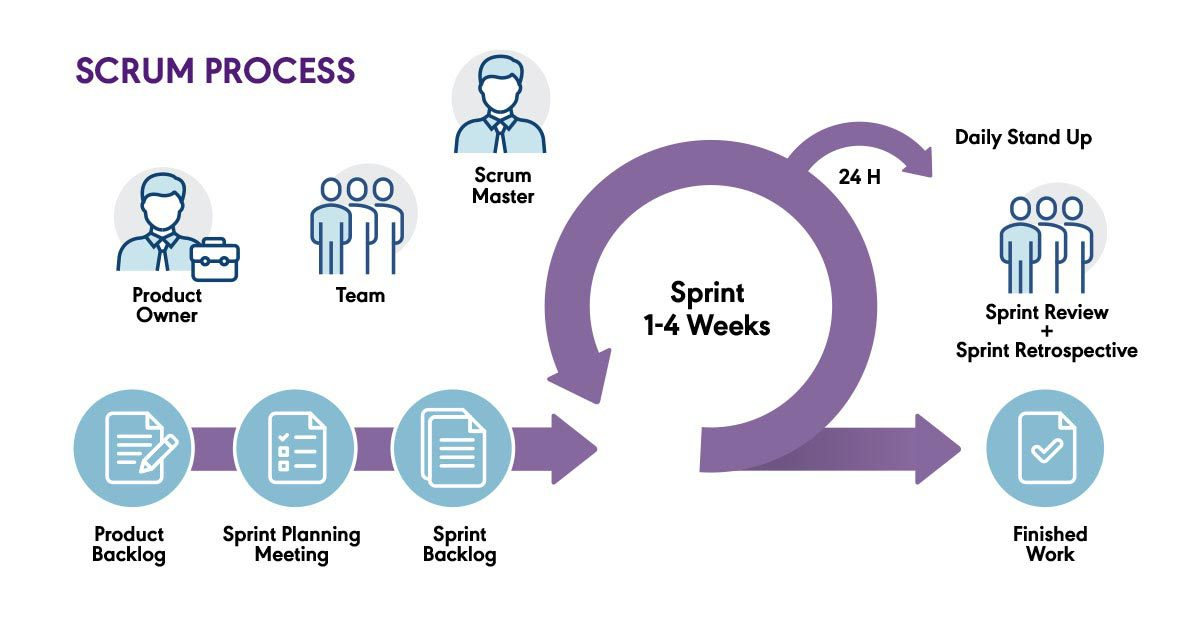
\includegraphics[width=\textwidth]{scrum.jpg}
					\caption{Le fonctionnement de la méthode SCRUM\cite{pm-partners}}
					\label{fig:SCRUM}
				\end{figure}
				\FloatBarrier				


				\subsubsection{Langage de modélisation}

				\hspace{15pt} Un langage de modélisation est un langage artificiel utilisé pour exprimer des informations, des connaissances ou des systèmes dans une structure définie par un ensemble cohérent de règles. Ces règles permettent d'interpréter la signification des composants dans la structure. 

				Les langages de modelisation peuvent être graphiques ou textuels et sont utilisés dans diverses disciplines comme l'informatique, la gestion de l'information, la modélisation des processus d'affaires,le génie logiciel et l'ingénierie des systèmes.


				Le tableau \ref{tab:Lmodel} représente la comparaison entre deux langages de modélisation populaire UML et ERD.

				
				\begin{longtable}{|p{3cm}|p{5.5cm}|p{5.5cm}|} 
						\caption{Comparaison entre UML et ERD.} 
						\label{tab:Lmodel}\\ 
						\hline 
						LANGAGE & AVANTAGES & INCONVÉNIENTS\\ 
						\hline 
						\endfirsthead 	
						\caption[]{(Suite)}\\ 
						\hline 
						LANGAGE & AVANTAGES & INCONVÉNIENTS\\ 
						\hline 
						\endhead
						UML (Unified Modeling Language) &
						\begin{itemize}
							\item Standard international largement adopté.
							\item Supporte la modélisation orienté objet.
							\item Utilisé pour la conception et la documentation des systèmes logiciels complexes.
						\end{itemize}
						&
						\begin{itemize}
							\item Peut être complexe à apprendre et à maîtriser. 
							\item Nécessite des outils spécifiques pour la modélisation.
						\end{itemize}\\						
						\hline
						ERD (Entity Relashionship Diagram) &
						\begin{itemize}
							\item Simple et facile à comprendre.
							\item Idéal pour la modélisation des bases de données relationnelles.
							\item Utilisé pour représenter les entités et leurs relations.
						\end{itemize} &
						\begin{itemize}
							\item Limité à la modélisation des bases de données.
							\item Moins adapté pour la modélisation des systèmes logiciels complexes.
						\end{itemize} \\
						\hline
				    \end{longtable}

				\paragraph{Choix du langage de modélisation} 
			
				Nous avons choisi d'utiliser UML pour "Handeha Voyage" en raison de ses nombreux avantages. En tant que standard international, UML est largement adopté et supporte la modélisation orienté objet, ce qui est essentiel pour notre projet. De plus, UML permet de concevoir et de documenter des systèmes logiciels complèxes de manière claire et précise, facilitant ainsi la communication entre les membres de l'equipe et les parties prenantes.

				\paragraph{Présentation d'UML}

				UML (Unified Modeling Language) est un langage de modélisation standardisé utilisé en ingénierie logicielle pour visualiser la conception de systèmes. Il inclut divers types de diagrammes pour représenter différents aspects d'un système, comme les diagrammes de classes, les diagrammes de cas d'utilisation et les diagrammes de séquence.

				Le développement de l'UML a commencé au milieu des années 1990 grâce aux travaux de Grady Booch, Ivar Jacobson et James Rumbaugh chez Rational Software. En 1997, l'UML est devenu un standard de l'Object Management Group (OMG), facilitant la modélisation des systèmes logiciels complexes\cite{Bennett}.

				UML est essentiel pour :

				\begin{itemize}
					\item Modéliser les structures statiques d'un système à travers des diagrammes de classes;
					\item Représenter les interactions dynamiques à l'aide de diagrammes de séquence;
					\item Décrire le comportement des systèmes avec des diagrammes d'état;
					\item Illustrer les cas d'utilisation pour définir les interactions entre les utilisateurs et le système.
				\end{itemize}

				\subparagraph{Diagrammes UML et leurs Utilités}
					
				Une des forces d'UML réside dans sa capacité à offrir une variété de diagrammes, chacun adapté à un aspect spécifique de la conception du système. Que ce soit pour illustrer la structure statique, les interactions dynamiques ou les flux de données, UML propose des outils visuels adaptés à chaque besoin.

				\begin{itemize}
					\item \textbf{Diagramme de Classe:} Montre la structure statique d'un système en représentant les classes, leurs attributs, méthodes et les relations entre elles;
					\item \textbf{Diagramme de Cas d'Utilisation:} Décrit les interactions entre les utilisateurs (acteurs) et le système à travers différents scénarios d'utilisation;
					\item \textbf{Diagramme de Séquence:} Illustre la séquence d'interactions entre les objets dans un scénario spécifique de l'application;
					\item \textbf{Diagramme d'État:} Représente les différents états d'un objet et les transitions entre ces états en réponse à des événements;
					\item \textbf{Diagramme d'Activité:} Montre le flux de contrôle ou de données à travers une série d'activités ou d'actions;
					\item \textbf{Diagramme de Composants:} Montre la décomposition d'un système en composants et les relations entre ces composants;
					\item \textbf{Diagramme de Déploiement:} Représente la configuration matérielle d'un système et les composants logiciels déployés sur ces matériels;
					\item \textbf{Diagramme d'Objet:} Montre une instance de classe et les relations entre ces instances à un moment donné.
				\end{itemize}
				


				\subsubsection{Outil de modélisation}

				\hspace{15pt} Les outils de modélisation sont des logiciels conçus pour aider les développeurs et les ingénieurs à visualiser, planifier et documenter les systèmes complexes. En fournissant une représentation graphique des systèmes, ces outils facilitent la communication entre les membres de l'équipe, permettent une meilleure compréhension des exigences et des architectures.

				Visual Paradigm et Astah sont deux outils de modélisation qui permettent tous deux de faire de l'UML.


				Le tableau \ref{tab:outilModelisation} représente la comparaison entre Visual Paradigm et Astah.


				\begin{longtable}{|p{3cm}|p{5.5cm}|p{5.5cm}|} 
						\caption{Comparaison  entre Visual Paradigm et Astah.} 
						\label{tab:outilModelisation}\\ 
						\hline 
						\textbf{Outil} & \textbf{Avantages} & \textbf{Inconvénients}\\ 
						\hline 
						\endfirsthead 	
						\caption[]{(Suite)}\\ 
						\hline 
						\textbf{Outil} & \textbf{Avantages} & \textbf{Inconvénients}\\ 
						\hline 
						\endhead
						Visual Paradigm &
						\begin{itemize}
							\item \textbf{Stabilité et Performance:} Connu pour sa stabilité et ses performances fiables;
							\item \textbf{Diversité de Diagrammes:} Offre une large gamme de diagrammes pour divers domaines de l'ingénierie;
							\item \textbf{Modélisation de Processus:} excellente pour la modélisation de processus avec simulation et animation;
							\item \textbf{Collaboration:} Support pour la collaboration en équipe avec des fonctionnalités de versioning et de gestion de projets;
							\item \textbf{Prix:} Modèle de prix attractif.
						\end{itemize} &
						\begin{itemize}
							\item \textbf{Compatibilité:} Peut avoir des difficultés à s'intégrer avec d'autres outils comme Atlassian Confluence;
							\item \textbf{Ressources:} Utilisation élevée des ressources, nécessitant des ordinateurs puissants;
							\item \textbf{Support Technique:} Le support technique peut être difficile à accéder ou inefficace pour certaines localisations;
							\item \textbf{Courbe d'apprentissage:} Peut présenter une courbe d'apprentissage raide, nécessitant parfois des services professionnels.
						\end{itemize}\\
						\hline
						Astah &
						\begin{itemize}
							\item \textbf{Facilité d'Utilisation:} Interface intuitive et facile à utiliser;
							\item \textbf{Polyvalence:} Supporte une large gamme de diagrammes UML et d'autres types de diagrammes;
							\item \textbf{Exportation et Importation:} Permet l'importation et l'exportation vers divers formats;
							\item \textbf{Plug-ins et Intégrations:} Personnalisation avec des plug-ins et intégrations;
							\item \textbf{Prix:} Options de prix flexibles, y compris une version gratuite pour les étudiants.
						\end{itemize} &
						\begin{itemize}
							\item \textbf{Exportation Limitée:} Peut manquer de certaines options d'exportation pour d'autres langages de programmation;
							\item \textbf{Contrôle de Version:} Peut avoir des limitations dans le contrôle de version pour les lignes de produits UML;
							\item \textbf{Support Technique:} Certaines fonctionnalités peuvent nécessiter des plug-ins supplémentaires.
						\end{itemize}\\						
						\hline
				    \end{longtable}


				\paragraph{Choix de l'outil de modélisation}
				
				Nous avons utilisé Visual Paradigm pour modéliser le projet Handeha Voyage en raison de ses fonctionnalités robustes et de sa capacité à offrir une représentation visuelle claire et structurée des différents aspects du système. Ses capacités de collaboration et de documentation avancées ont grandement facilité la communication et la gestion du projet tout au long du développement.


				\paragraph{Présentation de Visual Paradigm}

				Visual Paradigm est un outil de modélisation et de gestion de projet puissant et polyvalent, utilisé par les professionnels pour créer des diagrammes UML, BPMN et d'autres modèles de processus et de données. Il offre une interface intuitive et des fonctionnalités avancées telles que la collaboration en temps réel, la gestion des versions, et la génération automatique de code à partir des modèles.

				Visual Paradigm a été créé en 2002 par Visual Paradigm International Ltd., une société basée à Hong Kong. Depuis sa création, Visual Paradigm a évolué pour devenir un outil de modélisation puissant et complet, utilisé par des professionnels du monde entier pour la conception et la gestion de systèmes logiciels \cite{VisualParadigm}.

				Grâce à sa capacité à s'intégrer parfaitement avec divers environnements de développement et à ses options de personnalisation, Visual Paradigm est idéal pour les équipes cherchant à améliorer la communication, la documentation et la qualité globale de leurs projets logiciel

				\subsubsection{Système de Gestion de Base de Données}

				\hspace{15pt} Un système de gestion de base de données (SGBD) est un logiciel qui permet à un ordinateur de stocker, récupérer, ajouter, supprimer et modifier des données, tout en assurant la sécurité, l'intégrité des données et l'uniformité des procédures administratives.


				Le tableau \ref{tab:DBcomp} représente la comparaison entre MySQL et PostgreSQL.

				\begin{longtable}{|p{3cm}|p{5.5cm}|p{5.5cm}|} 
						\caption{Comparaison entre MySQL et PostgreSQL.} 
						\label{tab:DBcomp}\\ 
						\hline 
						SGBD & AVANTAGES & INCONVÉNIENTS\\ 
						\hline 
						\endfirsthead 	
						\caption[]{(Suite)}\\ 
						\hline 
						SGBD & AVANTAGES & INCONVÉNIENTS\\ 
						\hline 
						\endhead
						MySQL. &
						\begin{itemize}
							\item \textbf{Facilité d'utilisation:} Connu pour sa simplicité et sa facilité d'utilisation, ce qui en fait un choix populaire pour les applications web.
							\item \textbf{Scalabilité:} Gère efficacement de grands ensembles de données et des sites à fort trafic.
							\item \textbf{Support communautaire:} Support communautaire étendu et large gamme d'outils d'administration.
							\item \textbf{Performance:}  Généralement meilleur pour les charges de travail intensives en écriture.
						\end{itemize}
						&
						\begin{itemize}
							\item \textbf{Fonctionnalités limitées:} Moins flexible avec les requêtes complexes et dispose de moins de fonctionnalités avancées comparé à PostgreSQL.
							\item \textbf{Problèmes de verrouillage:} Peut rencontrer des problèmes de verrouillage sous des charges de travail très concurrentielles.
							\item \textbf{Moins d'extensibilité:} Offre moins d'options pour les extensions personnalisées par rapport à PostgreSQL.
						\end{itemize}\\						
						\hline
						PostgreSQL &
						\begin{itemize}
							\item \textbf{Conformité ACID:} Assure l'intégrité des données grâce à l'atomicité, la cohérence, l'isolation et la durabilité.
							\item \textbf{Fonctionnalités avancées:} Supporte les requêtes complexes, JSON, la recherche en texte intégral et les fonctions personnalisées.
							\item \textbf{Contrôle de la concurrence:} Excellent pour gérer plusieurs transactions simultanément sans problèmes de verrouillage.
							\item \textbf{Extensibilité:} Permet l'ajout de fonctions personnalisées et d'extensions.
							\item \textbf{Intégrité des données:} Fort support des types de données, des contraintes et de la validation.
						\end{itemize} &
						\begin{itemize}
							\item \textbf{Configuration complexe:} Plus complexe à installer et à configurer par rapport à des bases de données plus simples.
							\item \textbf{Surcharge de performance:} Peut être plus lent pour des applications simples et de petite échelle en raison de sa robustesse.
							\item \textbf{Intensif en ressources:} Nécessite plus de ressources système pour fonctionner efficacement, surtout sous forte charge.
						\end{itemize} \\
						\hline
				    \end{longtable}

				\paragraph{Choix du SGBD} 
				
				 PostgreSQL a été choisi pour l'environnement de production de l'application "Handeha Voyage" en raison de ses fonctionnalités avancées, de sa conformité ACID, et de sa capacité à gérer des transactions complexes et de grandes quantités de données de manière fiable. Son extensibilité et son support pour des requêtes complexes en font le candidat idéal pour une application de gestion et de promotion touristique qui nécessite une manipulation rigoureuse et sécurisée des données.

				\paragraph{Présentation de postgreSQL}

				PostgreSQL est un système de gestion de base de données relationnelle orienté objet, puissant et open source. Conçu pour être hautement extensible et conforme aux normes SQL, PostgreSQL est capable de gérer des charges de travail complexes et variées avec une grande fiabilité et des performances optimales. Utilisé par des entreprises à travers le monde, PostgreSQL est apprécié pour ses fonctionnalités avancées, sa stabilité et son support actif par la communauté.

				PostgreSQL a été créé en 1996 par Michael Stonebraker et son équipe à l'Université de Californie à Berkeley. Initialement appelé Postgres, il a été renommé PostgreSQL en 1996 pour refléter son adoption des normes SQL. Depuis, PostgreSQL est devenu l'une des bases de données relationnelles et objet les plus populaires et est soutenu par une communauté mondiale de développeur \cite{PostgreSQLExperience}.

				Voici quelques points clés qui illustrent pourquoi PostgreSQL est largement adopté par les entreprises du monde entier :

				\begin{itemize}
					\item \textbf{Extensibilité:} PostgreSQL permet aux utilisateurs de définir leurs propres types de données, fonctions, opérateurs et méthodes d'indexation, rendant le système extrêmement flexible et adapté à des besoins spécifiques.
					\item \textbf{Sécurité:} Avec des fonctionnalités de sécurité avancées, telles que le chiffrement SSL, l'authentification basée sur des rôles et le contrôle d'accès granulaire, PostgreSQL assure la protection des données sensibles.
					\item \textbf{Support pour les Transactions ACID:} PostgreSQL est conforme aux transactions ACID (Atomicity, Consistency, Isolation, Durability), garantissant une gestion fiable et sécurisée des transactions.
					\item \textbf{Haute Disponibilité:} Il supporte des configurations de haute disponibilité, y compris la réplication synchrone et asynchrone, les sauvegardes point-in-time et le failover, assurant ainsi la continuité des opérations.
					\item \textbf{Performance et Optimisation:} Grâce à des fonctionnalités telles que les index multi-colonnes, les index GIN/GIST, les plans d'exécution optimisés et le partitionnement, PostgreSQL est conçu pour des performances optimales, même sous des charges lourdes.
					\item \textbf{Communauté et Support:} PostgreSQL bénéficie d'une communauté active et d'un support abondant, avec de nombreuses ressources en ligne, forums et contributions régulières au code source, assurant une évolution continue et un support constant.
				\end{itemize}

				\subsubsection{Langages et choix du frameworks utilisés}

				\hspace{15pt} Pour assurer le succès et la robustesse d'un projet, il est essentiel de sélectionner des langages de programmation et des frameworks adaptés. Un langage de programmation est un ensemble de règles et de syntaxes que les développeurs utilisent pour écrire des programmes informatiques, tandis qu'un framework est une structure préétablie qui fournit un environnement de développement, simplifiant et standardisant le processus de création d'applications.


				\paragraph{Back-end}
				
				Le backend désigne la partie d'un système logiciel ou d'une application qui gère la logique, la base de données, et les opérations côté serveur.

				Le tableau \ref{tab:backend} représente la comparaison entre deux langages de programmation populaire pour faire du backend Java et C\#.
				
				\begin{longtable}{|p{3cm}|p{5.5cm}|p{5.5cm}|} 
						\caption{Comparaison entre Java et C\#.} 
						\label{tab:backend}\\ 
						\hline 
						\textbf{Langage} & \textbf{Avantages} & \textbf{Inconvénient}\\ 
						\hline 
						\endfirsthead 	
						\caption[]{(Suite)}\\ 
						\hline 
						\textbf{Langage} & \textbf{Avantages} & \textbf{Inconvénient}\\ 
						\hline 
						\endhead
						Java&
						\begin{itemize}
							\item Indépendant de la plateforme, grâce à la Java Virtual Machine (JVM).
							\item Performance et efficacité robustes pour les applications côté serveur.
							\item Vaste bibliothèque et cadres disponibles pour le développement.
							\item Fonctionnalités de sécurité élevées, essentielles pour gérer les données utilisateurs et les transactions financières.
						\end{itemize}
						&
						\begin{itemize}
							\item Courbe d'apprentissage plus raide comparée à certains autres langages.
							\item Code plus verbeux, ce qui peut ralentir la vitesse de développement.
						\end{itemize}\\						
						\hline
						C\# &
						\begin{itemize}
							\item Intégré de manière fluide avec les technologies Microsoft, parfait pour des applications Windows et cloud.
							\item Performance élevée et gestion de la mémoire efficace.
							\item Syntaxe similaire à Java, ce qui facilite l'apprentissage pour les développeurs Java.
							\item Grand écosystème avec des frameworks puissants pour le développement multi-plateforme.
						\end{itemize} &
						\begin{itemize}
							\item Principalement associé à l'écosystème Microsoft, ce qui peut limiter l'adoption sur certaines plateformes non-Microsoft.
							\item Courbe d'apprentissage pour certains frameworks spécifiques.
						\end{itemize} \\
						\hline
				    \end{longtable}

				\subparagraph{Choix des langages de programmation} 

				Java a été choisi pour le back-end de l'application "Handeha Voyage" en raison de ses performances robustes, de sa sécurité et de sa scalabilité. Sa capacité à gérer des opérations complexes et de grands volumes de transactions en fait une solution idéale pour gérer les processus de réservation, les données utilisateurs et les transactions financières.

				\subparagraph{Présentation de Java} 

				Java est un langage de programmation orienté objet, développé par Sun Microsystems (maintenant propriété d'Oracle) et publié pour la première fois en 1995. Java est conçu pour avoir le moins de dépendances possibles, ce qui permet aux développeurs de "écrire une fois, exécuter partout"\cite{Eckel}.

				Caractéristiques Principales:

				\begin{itemize}
					\item \textbf{Orienté Objet:} Java permet de structurer les logiciels en composants réutilisables et interconnectés;
					\item \textbf{Portabilité:} Les programmes Java sont compilés en bytecode, qui peut être exécuté sur toute machine disposant d'une Java Virtual Machine (JVM);
					\item \textbf{Sécurité:} Java inclut des fonctionnalités avancées de gestion des permissions et de sécurisation des données;
					\item \textbf{Multithreading:} Java facilite le développement de programmes capables de réaliser plusieurs tâches simultanément;
					\item \textbf{Richesse de l'Écosystème:} Un grand nombre de bibliothèques et de frameworks, tels que Spring et Hibernate, soutiennent le développement avec Java.
				\end{itemize}

				Utilisation Courante:
			
				Java est utilisé dans une variété de contextes, incluant le développement de :

				\begin{itemize}
					\item Applications d'entreprise;	
					\item Applications Android;
					\item Systèmes embarqués;
					\item Applications de bureau;
					\item Serveurs web et middleware;
				\end{itemize}

				Avec sa combinaison de robustesse, de sécurité et de portabilité, Java continue d'être un choix populaire pour le développement d'applications à grande échelle et critiques pour les entreprises.

				\subparagraph{Choix du framework}
			
				Le tableau \ref{tab:frameworkBack} représente la comparaison entre deux Framework Java populaire Spring Framework et Struts.
				
				\begin{longtable}{|p{3cm}|p{5.5cm}|p{5.5cm}|} 
						\caption{Comparaison entre Spring Framework et Struts.} 
						\label{tab:frameworkBack}\\ 
						\hline 
						\textbf{Framework}  & \textbf{Avantages} & \textbf{Inconvénient}\\ 
						\hline 
						\endfirsthead 	
						\caption[]{(Suite)}\\ 
						\hline 
						\textbf{Framework}  & \textbf{Avantages} & \textbf{Inconvénient}\\ 
						\hline 
						\endhead
						Spring Framework&
						\begin{itemize}
							\item \textbf{Flexibilité:} Très flexible avec de nombreuses options de configuration, permet l'injection de dépendances et une gestion simplifiée des objets.
							\item \textbf{Modularité:} Offre une structure modulaire, permettant aux développeurs de choisir uniquement les modules dont ils ont besoin.
							\item \textbf{Écosystème Riche:} Intégration facile avec de nombreux autres frameworks et bibliothèques.
							\item \textbf{Communauté et Documentation:} Grande communauté de développeurs et documentation abondante, facilitant la résolution des problèmes et l'apprentissage.
							\item \textbf{Spring Boot:} Simplifie encore plus le développement avec des configurations par défaut et des démarrages rapides.
						\end{itemize}
						&
						\begin{itemize}
							\item \textbf{Courbe d'Apprentissage:} Peut être complexe à apprendre pour les débutants en raison de sa richesse fonctionnelle.
							\item \textbf{Configuration:} La configuration peut devenir complexe pour des projets très personnalisés.
							\item \textbf{Abstraction:} Le niveau d'abstraction élevé peut rendre le débogage plus difficile.
						\end{itemize}\\						
						\hline
						Struts&
						\begin{itemize}
							\item \textbf{MVC (Model-View-Controller):} Suit le modèle MVC, ce qui aide à séparer la logique métier de la présentation.
							\item \textbf{Stabilité:} Étant l'un des plus anciens frameworks Java, il est très stable et mature.
							\item \textbf{Composants Réutilisables:} Offre des composants réutilisables, ce qui peut accélérer le développement.
							\item \textbf{Communauté:} A une communauté active qui maintient et améliore le framework.
						\end{itemize} &
						\begin{itemize}
							\item \textbf{Complexité:} Moins flexible et plus rigide que Spring, ce qui peut compliquer certaines personnalisations.
							\item \textbf{Configuration Manuelle:} Nécessite souvent une configuration manuelle plus détaillée par rapport à Spring Boot.
							\item \textbf{Évolutivité:} Moins bien adapté aux architectures modernes comme les microservices.
							\item \textbf{Performance:} Peut être moins performant pour les applications à grande échelle par rapport à Spring.
						\end{itemize} \\
						\hline
				    \end{longtable}

				\hspace{15pt} Pour l'application "Handeha Voyage", nous avons choisi Spring Framework avec Spring Boot pour sa flexibilité, sa modularité et sa capacité à intégrer facilement d'autres technologies. Spring Boot facilite le démarrage rapide et la gestion de l'application, ce qui nous permet de développer une solution robuste, évolutive et sécurisée.

				\subparagraph{Présentation de Spring Framework et Spring Boot}

				Spring Framework est un framework open source pour construire des applications Java et des services web. Développé par VMware, il a été publié pour la première fois en 2003. Spring est conçu pour simplifier le développement et les tests en fournissant une infrastructure modulaire et flexible\cite{SpringFramework}.

				Caractéristiques principales:
				
				\begin{itemize}
					\item \textbf{Inversion de contrôle (IoC):} Spring permet de gérer les dépendances via l'injection de dépendances, ce qui rend le code plus modulaire et facile à maintenir;
					\item \textbf{Couche d'abstraction:} Spring fournit des abstractions pour diverses technologies, facilitant l'intégration avec d'autres frameworks et bibliothèques;
					\item \textbf{Support pour les transactions:} Spring gère les transactions de manière transparente, ce qui simplifie la gestion des bases de données;
					\item \textbf{Sécurité:} Spring offre des fonctionnalités de sécurité avancées, telles que l'authentification et l'autorisation.
				\end{itemize}

				\subparagraph{Spring Boot}

				Spring Boot est une extension de Spring Framework qui simplifie le démarrage et le développement d'applications Spring. Il offre une configuration automatique et des "starters" pour inclure les dépendances nécessaires.

				Caractéristiques principales de Spring Boot:
				
				\begin{itemize}
					\item \textbf{Configuration automatique:} Spring Boot configure automatiquement l'application en fonction des dépendances présentes dans le classpath;
					\item \textbf{Starters:} Des modules préconfigurés qui simplifient l'intégration de Spring avec des technologies spécifiques, comme Spring MVC pour les applications web ou Spring Data pour les bases de données;
					\item \textbf{Packaging autonome:} Spring Boot permet de créer des applications autonomes pouvant être exécutées en tant que fichiers JAR ou WAR;
					\item \textbf{Microservices:} Idéal pour le développement de microservices, Spring Boot facilite la création et le déploiement de services indépendants.
				\end{itemize}

				\paragraph{Front-end}

				Le frontend désigne la partie d'un site web ou d'une application qui interagit directement avec l'utilisateur. C'est tout ce que l'utilisateur voit et avec lequel il interagit sur son écran. Le frontend est responsable de l'apparence visuelle, de l'ergonomie et de l'expérience utilisateur.				

				Le tableau \ref{tab:front} représente la comparaison entre  deux langages de programmation populaire pour faire du Front-end JavaScript et Elm.


				\begin{longtable}{|p{3cm}|p{5.5cm}|p{5.5cm}|} 
						\caption{Comparaison entre JavaScript et Elm.} 
						\label{tab:front}\\ 
						\hline 
						\textbf{Langage} & \textbf{Avantages} & \textbf{Inconvénient}\\ 
						\hline 
						\endfirsthead 	
						\caption[]{(Suite)}\\ 
						\hline 
						\textbf{Langage} & \textbf{Avantages} & \textbf{Inconvénient}\\ 
						\hline 
						\endhead
						JavaScript&
						\begin{itemize}
							\item \textbf{Popularité et Écosystème:} Énorme communauté, abondance de bibliothèques et de frameworks (comme React, Angular, et Vue);
							\item \textbf{Flexibilité:} Langage dynamique avec une syntaxe souple qui permet un développement rapide;
							\item \textbf{Interopérabilité:} Pratiquement tous les navigateurs modernes supportent JavaScript nativement.
						\end{itemize}
						&
						\begin{itemize}
							\item \textbf{Gestion des Erreurs:} JavaScript étant un langage non typé, les erreurs ne sont souvent détectées qu'à l'exécution;
							\item \textbf{Performance:} Bien que performant, il peut être moins optimisé que certains autres langages spécialisés;
							\item \textbf{Complexité:} La flexibilité excessive peut mener à des pratiques de codage inconsistantes et des bugs difficiles à traquer.
						\end{itemize}\\						
						\hline
						Elm&
						\begin{itemize}
							\item \textbf{Sécurité:} Élimine pratiquement les erreurs d'exécution grâce à un système de types strict;
							\item \textbf{Simplicité et Cohérence:} Syntaxe propre et claire, favorisant un code lisible et maintenable;
							\item \textbf{Expérience Développeur:} Excellent support pour le refactoring de code et une gestion des erreurs claire et informative.
						\end{itemize} &
						\begin{itemize}
							\item \textbf{Écosystème:} Moins de bibliothèques et de ressources comparé à JavaScript, ce qui peut limiter certaines fonctionnalités;
							\item \textbf{Courbe d'Apprentissage:} Peut nécessiter une période d'apprentissage plus longue pour les développeurs non familiers avec la programmation fonctionnelle;
							\item \textbf{Interopérabilité:} Bien que compatible avec JavaScript, l'intégration avec des projets existants peut nécessiter des efforts supplémentaires.
						\end{itemize} \\
						\hline
				    \end{longtable}

				\subparagraph{Choix du langage front-end}

				Nous avons choisi JavaScript pour le frontend du projet Handeha Voyage car il est largement populaire, fonctionne nativement dans tous les navigateurs web modernes, offre des performances optimisées grâce aux moteurs JavaScript récents, est flexible pour ajouter des fonctionnalités interactives, et s'intègre facilement avec d'autres technologies et services web, assurant ainsi une application robuste et conviviale.

				\subparagraph{Présentation de JavaScript}

				JavaScript est un langage de programmation créé en 1995 par Brendan Eich chez Netscape Communications Corporation. Initialement appelé Mocha, puis LiveScript, il a été renommé JavaScript pour capitaliser sur la popularité de Java. JavaScript a été standardisé sous le nom d'ECMAScript en 1997. Depuis, il est devenu un élément central des applications web, utilisé pour ajouter de l'interactivité et des fonctionnalités dynamiques aux pages web \cite{JavaScriptHistory}.

				Points Clés:

				\begin{itemize}
					\item \textbf{Polyvalence:} JavaScript peut être utilisé côté client (dans le navigateur) et côté serveur (avec Node.js);
					\item \textbf{Écosystème Étendu:} De nombreux frameworks et bibliothèques comme React, Angular, et Vue.js facilitent le développement d'applications web complexes;
					\item \textbf{Compatibilité:} Il est pris en charge par tous les navigateurs modernes, assurant une large portée;
					\item \textbf{Performance:} Les moteurs JavaScript modernes comme V8 (Chrome) et SpiderMonkey (Firefox) offrent des performances optimisées.
				\end{itemize}

				\subparagraph{Choix du framework}

				Le tableau \ref{tab:frameworkFront} représente la comparaison entre deux Framework JavaScript populaire Next.js et Vue.js.
				
				\begin{longtable}{|p{3cm}|p{5.5cm}|p{5.5cm}|} 
						\caption{Comparaison entre Next.js et Vue.js.} 
						\label{tab:frameworkFront}\\ 
						\hline 
						\textbf{Framework}  & \textbf{Avantages} & \textbf{Inconvénient}\\ 
						\hline 
						\endfirsthead 	
						\caption[]{(Suite)}\\ 
						\hline 
						\textbf{Framework}  & \textbf{Avantages} & \textbf{Inconvénient}\\ 
						\hline 
						\endhead
						Next.js&
						\begin{itemize}
							\item \textbf{Performance et SEO:} Le SSR et le SSG permettent des chargements de pages plus rapides et une meilleure visibilité dans les moteurs de recherche;
							\item \textbf{Simplicité du Routage:} Utilise un système de routage basé sur le système de fichiers, ce qui simplifie la gestion des routes;
							\item \textbf{Fonctionnalités Full-Stack:} Les routes API permettent de gérer facilement les requêtes backend, facilitant le développement d'applications full-stack;
							\item \textbf{Intégration Native avec TypeScript:} Offre un support excellent pour TypeScript, assurant un code plus robuste et plus sûr.
						\end{itemize}
						&
						\begin{itemize}
							\item \textbf{Courbe d'Apprentissage:} Peut être difficile à maîtriser pour les développeurs débutants ou ceux non familiers avec React;
							\item \textbf{Configuration Initiale:} Bien que moins complexe que d'autres solutions, la configuration initiale peut encore nécessiter des ajustements pour les projets spécifiques;
							\item \textbf{Dépendance à React:} Nécessite une bonne connaissance de React, ce qui peut être une barrière pour les équipes non formées à cet écosystème.
						\end{itemize}\\						
						\hline
						Vue.js&
						\begin{itemize}
							\item \textbf{Simplicité et Accessibilité:} Facile à apprendre pour les développeurs débutants grâce à sa syntaxe intuitive et sa documentation exhaustive.
							\item \textbf{Flexibilité:} Peut être utilisé progressivement ou intégré avec d'autres projets existants sans nécessiter une refonte complète.
							\item \textbf{Performance:} Utilise un DOM virtuel pour des mises à jour efficaces et rapides de l'interface utilisateur;
							\item \textbf{Écosystème:} Dispose de nombreux plugins et extensions qui enrichissent les fonctionnalités sans alourdir le développement.
						\end{itemize} &
						\begin{itemize}
							\item \textbf{Écosystème Moins Mature:} Comparé à React, l'écosystème de Vue.js est encore en croissance, avec moins de ressources et de bibliothèques disponibles;
							\item \textbf{Support Entreprises:} Moins de soutien et d'adoption par les grandes entreprises comparé à React et Angular, ce qui peut poser des défis pour des projets à grande échelle;
							\item \textbf{Complexité Croissante:} Pour les projets très complexes, Vue.js peut devenir difficile à maintenir sans une structure et une gestion rigoureuses.
						\end{itemize} \\
						\hline
				    \end{longtable}

				Nous avons choisi Next.js pour son rendu côté serveur (SSR) et la génération de sites statiques (SSG), qui améliorent les performances de l'application et optimisent le référencement (SEO), ainsi que pour sa gestion simplifiée des routes et ses fonctionnalités full-stack facilitant le développement d'API.

				\subparagraph{Présentation de Next js}

				Next.js est un framework open-source de développement web créé par Vercel en 2016. Il est basé sur React et permet de construire des applications web avec des fonctionnalités supplémentaires telles que le rendu côté serveur et la génération de sites statiques. Next.js simplifie le développement en offrant une infrastructure modulaire et flexible, permettant aux développeurs de se concentrer sur la création de leur application plutôt que sur la configuration \cite{NextJS}.

				Caractéristiques Principales:

				 \begin{itemize}
					\item \textbf{Rendu Côté Serveur (SSR):} Permet de générer des pages HTML complètes sur le serveur avant de les envoyer au navigateur, améliorant les performances et le référencement;
					\item \textbf{Rendu Statique (SSG):} Permet de générer des pages HTML statiques lors du build, ce qui réduit les temps de chargement et améliore l'expérience utilisateur;
					\item \textbf{Système de Routage Basé sur le Système de Fichiers:} Simplifie la gestion des routes en utilisant des fichiers pour chaque page, facilitant la création de routes dynamiques;
					\item \textbf{Support TypeScript} Intégration native du TypeScript pour un typage fort et une meilleure gestion des erreurs;
					\item \textbf{Optimisations d'Images et de Scripts} Pré-configuration des optimisations pour améliorer les vitesses de chargement et l'expérience utilisateur.
				\end{itemize}


				\subsubsection{Choix de l’environnement de développement}
				
				\hspace{15pt} Un environnement de développement intégré (IDE) est un logiciel qui combine des outils de développement nécessaires pour écrire, tester, et déboguer du code. Les IDE offrent généralement un éditeur de code source, des outils de construction automatisés et un débogueur. Les fonctionnalités additionnelles peuvent inclure la complétion de code, la gestion de projets, l’intégration avec des systèmes de contrôle de version et des outils de déploiement.

				Les environnements de développement sont essentiels pour les développeurs, car ils fournissent une interface unifiée qui simplifie les différentes tâches du cycle de développement logiciel.

				Le tableau \ref{tab:IDE} représente la comparaison entre Visual Studio Code, Eclipse, IntelliJ IDEA et Atom.
				
				\begin{longtable}{|p{3cm}|p{5.5cm}|p{5.5cm}|} 
						\caption{Comparaison entre Visual Studio Code, Eclipse, IntelliJ IDEA et Atom.} 
						\label{tab:IDE}\\ 
						\hline 
						\textbf{IDE}  & \textbf{Avantages} & \textbf{Inconvénient}\\ 
						\hline 
						\endfirsthead 	
						\caption[]{(Suite)}\\ 
						\hline 
						\textbf{IDE}  & \textbf{Avantages} & \textbf{Inconvénient}\\ 
						\hline 
						\endhead
						Visual Studio Code &
						\begin{itemize}
							\item Léger et rapide;
							\item Hautement personnalisable avec une grande variété d'extensions;
							\item Intégration Git intégrée;
							\item Supporte de nombreux langages de programmation.
						\end{itemize}
						&
						\begin{itemize}
							\item Peut être limité pour les projets très complexes;
							\item Certaines extensions peuvent ralentir l'éditeur;
							\item Pas autant de fonctionnalités avancées intégrées par défaut comparé à des IDE plus complets.
						\end{itemize}\\
						\hline
						Eclipse & 
						\begin{itemize}
							\item Très puissant et riche en fonctionnalités;
							\item Supporte de nombreux langages de programmation via des plugins;
							\item Communauté active et grand nombre de ressources;
							\item Mise à jour régulière et support de longue durée.
						\end{itemize}
						&
						\begin{itemize}
							\item Peut être lourd et consommer beaucoup de ressources système;
							\item Courbe d'apprentissage plus élevée pour les débutants;
							\item Moins de personnalisation de l'interface par rapport à VS Code;
							\item Nécessite souvent des configurations supplémentaires pour certains langages ou projets.
						\end{itemize}\\
						 \hline
						Atom & 
						\begin{itemize}
							\item Très personnalisable avec de nombreuses extensions;
							\item Interface propre et moderne;
							\item Gratuit et open-source.
						\end{itemize}
						&
						\begin{itemize}
							\item Peut être plus lent avec de gros fichiers ou projets;
							\item Moins de fonctionnalités intégrées comparé à VS Code.
						\end{itemize}\\
						 \hline
						IntelliJ IDEA & 
						\begin{itemize}
							\item Excellente intégration avec les frameworks populaires de Java;
							\item Fonctions de refactoring puissantes;
							\item Complétion de code intelligente.
						\end{itemize}
						&
						\begin{itemize}
							\item Peut être lourd et lent à démarrer;
							\item La version complète est payante.
						\end{itemize}\\
						\hline

				    \end{longtable}


				Nous avons choisi d'utiliser Visual Studio Code pour le développement front-end avec Next.jsen raison de sa légèreté, de sa personnalisation facile et de son intégration parfaite avec les technologies front-end modernes, et Eclipse pour le développement back-end avec Java en raison de sa robustesse, de ses fonctionnalités complètes et de son support excellent pour les projets Java complexes.


				\subsubsection{Système de contrôle de version}

				\hspace{15pt} Un système de contrôle de version (VCS) est un outil essentiel pour la gestion des changements apportés aux documents, programmes, et autres collections d'informations. Les VCS permettent aux développeurs de suivre les modifications du code source, de collaborer avec d'autres développeurs et de revenir à des versions antérieures si nécessaire. Ils facilitent également la gestion des branches de développement et l'intégration de différentes contributions.


				Le tableau \ref{tab:VCS} représente la comparaison entre Git et SVN.
				
				\begin{longtable}{|p{3cm}|p{5.5cm}|p{5.5cm}|} 
						\caption{Comparaison entre Git et SVN.} 
						\label{tab:VCS}\\ 
						\hline 
						\textbf{VCS}  & \textbf{Avantages} & \textbf{Inconvénient}\\ 
						\hline 
						\endfirsthead 	
						\caption[]{(Suite)}\\ 
						\hline 
						\textbf{VCS}  & \textbf{Avantages} & \textbf{Inconvénient}\\ 
						\hline 
						\endhead
						Git &
						\begin{itemize}
							\item Distribué, permettant un travail en déconnecté;
							\item Gestion efficace des branches et des fusions;
							\item Performance rapide;
							\item Large adoption et soutien communautaire.
						\end{itemize}
						&
						\begin{itemize}
							\item Courbe d'apprentissage initiale pour les débutants;
							\item Complexité des commandes avancées.
						\end{itemize}\\
						\hline
						SVN & 
						\begin{itemize}
							\item Simple à configurer et à utiliser;
							\item Stabilité et fiabilité éprouvées;
							\item Gestion facile des versions centralisées;
							\item Bon support pour les fichiers binaires.
						\end{itemize}
						&
						\begin{itemize}
							\item Moins flexible que Git pour la gestion des branches;
							\item Travail déconnecté limité;
							\item Moins de popularité dans les nouveaux projets comparé à Git.
						\end{itemize} \\
						 \hline
				    \end{longtable}


				\paragraph{Choix du système de contrôle de version}
				
				Git est idéal pour les projets où la flexibilité, la performance et la gestion des branches sont essentielles. Sa capacité à permettre un travail déconnecté et à gérer efficacement les fusions en fait un choix parfait pour des projets avec des contributions multiples et des cycles de développement rapides.

				\paragraph{Présentation de Git}

				Git est un système de contrôle de version distribué, développé par Linus Torvalds en 2005 pour la gestion du code source du noyau Linux. Git est devenu le VCS le plus utilisé grâce à sa flexibilité, sa performance et son large soutien communautaire. Il permet aux développeurs de travailler en déconnecté, de créer des branches facilement et de gérer efficacement les fusions.

				Git permet de créer et de gérer des branches de développement de manière efficace. Il offre une performance rapide et une flexibilité accrue, facilitant la collaboration et la gestion des contributions. Git est largement adopté dans l'industrie, avec un écosystème riche comprenant des plateformes comme GitHub, GitLab et Bitbucket\cite{Tsitoara}.

				


				\subsubsection{Katappult, la plateforme low code}

				\hspace{15pt} Qu'est-ce que le low code ? Le low code est enfaite une approche innovante qui transforme le développement d'applications en facilitant la création rapide de solutions, tant pour les professionnels que pour les utilisateurs non techniques. Cette méthode repose sur des plateformes intuitives qui permettent aux utilisateurs de concevoir des applications via des interfaces visuelles et des fonctions de glisser-déposer, réduisant ainsi le besoin de codage manuel. Cela ouvre la voie à une \textbf{industrialisation du prototypage}, permettant de créer des applications plus rapidement et à moindre coût, tout en augmentant la qualité du produit final. Et au sein de NEXITIA TECHNOLOGIE, cette solution innovante est déjà exploitée pour accompagner la réalisation de ses projets avec sa propre plateforme low code Katappult.
	
				Katappult est une plateforme de développement low code qui illustre parfaitement l’essence même du low code avec ses avantages. Elle permet non seulement aux utilisateurs (clients) de créer facilement des applications web et mobiles grâce à une base robuste qui simplifie le processus de prototypage, et mais également offre un atout majeur en plus, la \textbf{possibilité d'accéder au code source pour une personnalisation avancée}, combinant ainsi rapidité et flexibilité \cite{katappult}. Ceci procure un avantage net aux clients, en effet par rapport aux autres plateformes low code la propriété intellectuelle de toute l’application est propriété du client et il peut le déployer dans n’importe quel cloud de son choix.

				Ainsi pour mettre en place les premières bases de notre projet, l’utilisation de Katappult a été plus que nécessaire.




				\chapter{ANALYSE CONCEPTUELLE}

				\hspace{15pt} Ce chapitre est consacré à étudier comment la méthode SCRUM est appliquée pour conduire le projet.

				\section{Désignation des rôles de l’équipe SCRUM}

				\hspace{15pt} Le projet "Handeha Voyage" adopte la méthodologie SCRUM pour garantir une gestion agile et efficace. SCRUM est un cadre de travail qui aide les équipes à structurer et à améliorer leurs processus de manière itérative et incrémentale. Il offre une base solide pour l'organisation des réunions, la gestion des artefacts, et la répartition des responsabilités, tout en laissant une flexibilité nécessaire pour s'adapter aux spécificités de chaque projet.

				Pour un projet de la complexité de "Handeha Voyage", il est essentiel de définir clairement les rôles au sein de l'équipe SCRUM. Ces rôles sont les suivants :

				\begin{itemize}
					\item \textbf{Membres de l'équipe de développement:} Ils sont responsables de la création et de la livraison des fonctionnalités du produit. L'équipe doit comprendre des experts en développement frontend et backend, ainsi que des spécialistes du domaine métier pour assurer une couverture complète des besoins du projet.
					\item \textbf{Product Owner:} Ce rôle est crucial pour la définition et la gestion des exigences du projet. Le Product Owner est responsable de la vision du produit et veille à ce que l'équipe de développement travaille sur les fonctionnalités ayant le plus de valeur pour les utilisateurs finaux.
					\item \textbf{Scrum Master:} Le Scrum Master est le facilitateur de l'équipe. Il garantit que les principes et pratiques SCRUM sont respectés et aide l'équipe à surmonter les obstacles et à améliorer continuellement ses processus.
				\end{itemize}
				
				En plus des membres traditionnels de l'équipe SCRUM, nous avons également inclus des professionnels issus des domaines du tourisme et de l'hôtellerie. Leur expertise est essentielle pour garantir que le projet "Handeha Voyage" répond aux besoins spécifiques et aux attentes des utilisateurs finaux. Ces professionnels apportent une connaissance approfondie des tendances du marché, des attentes des clients, et des meilleures pratiques dans le domaine du tourisme et de l'hôtellerie.

				\section{Etapes de l’élaboration du product backlog}

				\hspace{15pt} Le product backlog est un élément clé dans la gestion agile du projet "Handeha Voyage". Son élaboration permet de répondre à trois questions essentielles :

				\begin{itemize}
					\item Qui sont les utilisateurs ciblés ?
					\item Quelles fonctionnalités doivent être développées ?
					\item Quel sera l'ordre de livraison de ces fonctionnalités ?
				\end{itemize}

				Pour répondre à ces questions, nous suivons un processus en cinq étapes que nous allons détailler un à un.

				\subsection{Établissement de la vision du projet}

				\hspace{15pt} Cette étape consiste à définir les objectifs globaux et l'orientation stratégique du projet.

				Établir une plateforme de réservation touristique comme "Handeha Voyage" incluant : l'inscription et l'authentification sur la plateforme, la gestion des rôles et permissions des utilisateurs, la gestion des circuits et des séjours touristiques, la réservation des circuits et des séjours, le paiement des réservations, ainsi que la gestion des réservations et des paiements.

				\subsection{Liste des acteurs}

				\hspace{15pt} Il est nécessaire d'identifier et de détailler tous les intervenants et utilisateurs du système dans tous ses aspects. Pour chaque intervenant, les informations suivantes doivent être précisées : rôle, description, critère de satisfaction, fréquence d’utilisation, niveau de connaissance technologique et niveau de connaissance métier.

				Dans le cas d' Handeha Voyage, il existe cinque acteurs:

				\begin{itemize}
					\item Super Administrateur;
					\item Administrateur;
					\item Voyagiste;
					\item Voyageur.
					\item Utilisateur anonyme
				\end{itemize}

				La tableau \ref{tab:acteurSupAdm} représente le Super Administrateur.


				\begin{table}[h]
				  \centering
				  \caption{le Super Administrateur du projet Handeha Voyage.}
				  \label{tab:acteurSupAdm}
				    \begin{tabular}{|p{3cm}|p{4cm}|p{7cm}|}
					\hline
					\begin{minipage}{3cm}
						
\includegraphics[width=2cm]{supAdm.png}
					\end{minipage} & \textbf{Rôle} & Utilisateur de plus haut niveau responsable de l'administration, de la sécurité et de la configuration du système.\\ \cline{2-3}
							& \textbf{Description} & Gère les rôles des utilisateurs, les permissions, les Régions et les Thèmes. \\ \cline{2-3}
							& \textbf{Critère de satisfaction}& \begin{itemize}
														\item Stabilité et sécurité du système;
														\item Gestion efficace des utilisateurs, des rôles, des régions et des thèmes;
														\item Conformité aux politiques et réglementations.
													\end{itemize}\\ \cline{2-3}
							&\textbf{Fréquence d’utilisation} & Quotidienne \\  \cline{2-3}
							&\textbf{Niveau de Connaissance Technologique} & Elevée \\  \cline{2-3}
							&\textbf{Niveau de Connaissance Métier} & Elevée \\ 
					\hline
				    \end{tabular}
				\end{table}
				\FloatBarrier				

				La tableau \ref{tab:aAdmHandeha} représente l'Administrateur Handeha Voyage.


				\begin{table}[h]
				  \centering
				  \caption{l'Administrateur du projet Handeha Voyage.}
				  \label{tab:aAdmHandeha}
				    \begin{tabular}{|p{3cm}|p{4cm}|p{7cm}|}
					\hline
					\begin{minipage}{3cm}
						
\includegraphics[width=2cm]{adminHandeha.png}
					\end{minipage} & \textbf{Rôle} & Suivre les opérations quotidiennes de la plateforme de voyage.\\ \cline{2-3}
							& \textbf{Description} & Valider les demandes de validation de voyage, de publication de voyage, de devenir voyagiste et suivre les statistiques des opérations quotidiennes de la plateforme.  \\ \cline{2-3}
							& \textbf{Critère de satisfaction}& \begin{itemize}
														\item Haute satisfaction des clients et résolution rapide des problèmes.;
														\item Gestion rapide des demandes;
														\item Tableau de bord pour le suivis des statistiques.
													\end{itemize}\\ \cline{2-3}
							&\textbf{Fréquence d’utilisation} & Permanente \\  \cline{2-3}
							&\textbf{Niveau de Connaissance Technologique} & Elevée \\  \cline{2-3}
							&\textbf{Niveau de Connaissance Métier} & Elevée \\ 
					\hline
				    \end{tabular}
				\end{table}
				\FloatBarrier				

				La tableau \ref{tab:Voyagiste} représente le Voyagiste du projet Handeha Voyage.


				\begin{table}[h]
				  \centering
				  \caption{Voyagiste du projet Handeha Voyage.}
				  \label{tab:Voyagiste}
				    \begin{tabular}{|p{3cm}|p{4cm}|p{7cm}|}
					\hline
					\begin{minipage}{3cm}
						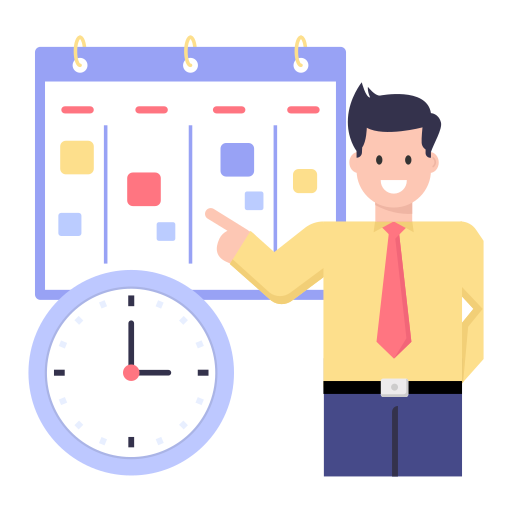
\includegraphics[width=2cm]{voyagiste.png}
					\end{minipage} & \textbf{Rôle} & Organise et planifie des forfaits de voyage\\ \cline{2-3}
							& \textbf{Description} & Gérer les circuits et séjours touristique, Gérer les réservations et paiements, Suivre les statistiques de leur offres \\ \cline{2-3}
							& \textbf{Critère de satisfaction}& \begin{itemize}
														\item Forfaits de voyage bien organisés et attrayants;
														\item Augmentation des réservations;
														\item Tableau de bord pour le suivis des statistiques de leur offres.
													\end{itemize}\\ \cline{2-3}
							&\textbf{Fréquence d’utilisation} & Quotidienne \\  \cline{2-3}
							&\textbf{Niveau de Connaissance Technologique} & Moyenne \\  \cline{2-3}
							&\textbf{Niveau de Connaissance Métier} & Elevée \\ 
					\hline
				    \end{tabular}
				\end{table}
				\FloatBarrier				


				La tableau \ref{tab:Voyageur} représente le Voyagiste du projet Handeha Voyage.


				\begin{table}[h]
				  \centering
				  \caption{Voyageur du projet Handeha Voyage.}
				  \label{tab:Voyageur}
				    \begin{tabular}{|p{3cm}|p{4cm}|p{7cm}|}
					\hline
					\begin{minipage}{3cm}
						
\includegraphics[width=2cm]{voyageur.png}
					\end{minipage} & \textbf{Rôle} & L'utilisateur final qui réserve et participe aux forfaits de voyage.\\ \cline{2-3}
							& \textbf{Description} & Utilise la plateforme pour trouver, réserver et payer ses plans de voyage\\ \cline{2-3}
							& \textbf{Critère de satisfaction}& \begin{itemize}
														\item Expérience de réservation facile et intuitive;
														\item Expériences de voyage agréables et sans tracas.
													\end{itemize}\\ \cline{2-3}
							&\textbf{Fréquence d’utilisation} & occasionnel \\  \cline{2-3}
							&\textbf{Niveau de Connaissance Technologique} & Basse \\  \cline{2-3}
							&\textbf{Niveau de Connaissance Métier} & Basse \\ 
					\hline
				    \end{tabular}
				\end{table}
				\FloatBarrier				

				La tableau \ref{tab:Anon} représente le Voyagiste du projet Handeha Voyage.


				\begin{table}[h]
				  \centering
				  \caption{Utilisateu anonyme du projet Handeha Voyage.}
				  \label{tab:Anon}
				    \begin{tabular}{|p{3cm}|p{4cm}|p{7cm}|}
					\hline
					\begin{minipage}{3cm}
						
\includegraphics[width=2cm]{anonyme.png}
					\end{minipage} & \textbf{Rôle} & Naviguer et consulter sur la plateforme.\\ \cline{2-3}
							& \textbf{Description} & Dispose d’un accès limité.\\ \cline{2-3}
							& \textbf{Critère de satisfaction}& \begin{itemize}
														\item Simplicité de navigation;
														\item Visionnage des offres sans engagement.
													\end{itemize}\\ \cline{2-3}
							&\textbf{Fréquence d’utilisation} & occasionnel \\  \cline{2-3}
							&\textbf{Niveau de Connaissance Technologique} & Basse \\  \cline{2-3}
							&\textbf{Niveau de Connaissance Métier} & Basse \\ 
					\hline
				    \end{tabular}
				\end{table}
				\FloatBarrier				


				\subsection{Thèmes}
				
				\hspace{15pt} Les thèmes sont des regroupements de fonctionnalités similaires qui permettent d'organiser le travail de manière cohérente. 
				
				De la vision du projet et la définition de chaque acteur, on extrait facilement les thèmes suivants :
				
				\begin{itemize}
					\item Inscription et authentification sur la plateforme
					\item Géstion des utilisateurs
					\item Géstion des rôles et des permissions
					\item Géstion des régions et les thèmes 							
					\item Gestion des demandes de devenir voyagiste
					\item Géstion des demandes de validation des circuits et séjours
					\item Géstion des demandes de publication des circuits et séjours 											
					\item Suivi des statistiques des opérations sur la plateforme
					\item Géstion des circuits et séjours
					\item Géstion des hébergements, des restaurations, des activités et des points d'intérêt des circuits et des séjours
					\item Demande de validation des circuits et séjours
					\item Demande de publication des circuits et séjours
					\item Géstion des réservations
					\item Suivi des paiements
					\item Suivi des statistiques des circuits et séjours
					\item Recherche des voyages
					\item Réservation des voyages
					\item Paiement des réservations
					\item Demande de devenir voyagiste							
					\item Demande d'annulation des réservations
				\end{itemize}

				\subsection{Vision de la première release}

				\hspace{15pt} La première release du projet "Handeha Voyage" se concentrera sur le thème ayant la plus haute priorité, assurant ainsi une base solide pour les fonctionnalités essentielles.

				Voici l'ordre de priorité des thèmes :

				\begin{itemize}
					\item \textbf{thème 1:} Inscription et authentification sur la plateforme
					\item \textbf{thème 2:} Gestion des utilisateurs
					\item \textbf{thème 3:} Gestion des rôles et des permissions
					\item \textbf{thème 4:} Gestion des régions et les thèmes
					\item \textbf{thème 5:} Gestion des circuits et séjours
					\item \textbf{thème 6:} Recherche des voyages
					\item \textbf{thème 7:} Réservation des voyages
					\item \textbf{thème 8:} Paiement des réservations
					\item \textbf{thème 9:} Demande d'annulation des réservations
					\item \textbf{thème 10:} Gestion des réservations
					\item \textbf{thème 11:} Suivi des paiements
					\item \textbf{thème 12:} Suivi des statistiques des opérations sur la plateforme
					\item \textbf{thème 13:} Suivi des statistiques des circuits et séjours
					\item \textbf{thème 14:} Gestion des demandes de devenir voyagiste
					\item \textbf{thème 15:} Gestion des demandes de validation des circuits et séjours
					\item \textbf{thème 16:} Gestion des demandes de publication des circuits et séjours
					\item \textbf{thème 17:} Gestion des hébergements, des restaurations, des activités et des points d'intérêt des circuits et des séjours
					\item \textbf{thème 18:} Demande de validation des circuits et séjours
					\item \textbf{thème 19:} Demande de publication des circuits et séjours
					\item \textbf{thème 20:} Demande de devenir voyagiste
				\end{itemize}

				La première release est "Inscription et authentification sur la plateforme".

				\subsection{User stories}

				\hspace{15pt} Pour comprendre les besoins et attentes des différents utilisateurs de la plateforme "Handeha Voyage", nous avons élaboré les histoires d’utilisateurs suivantes. Ces histoires permettent de capturer les fonctionnalités essentielles du point de vue des utilisateurs finaux, assurant que le développement reste centré sur l’expérience utilisateur. 

				Une User Story respecte la syntaxe suivante : En tant que …, je veux …, afin de …


				\begin{itemize}
					\item En tant qu'Utilisateur anonyme, je veux m'inscrire pour pouvoir accéder aux fonctionnalités de réservation et paiements de voyages. 
					\item En tant que Voyageur, je veux m'inscrire et m'authentifier pour accéder à mes informations de voyage personnalisées de manière sécurisée.
					\item En tant que Voyagiste, je veux pouvoir m'authentifier pour gérer mes circuits, séjours, et réservations de manière sécurisée.
					\item En tant qu'Administrateur Handeha Voyage, je veux pouvoir m'authentifier pour gérer les demandes et suivre les opérations de manière sécurisée.
					\item En tant que Super Administrateur, je veux pouvoir m'authentifier pour accéder aux fonctionnalités avancées de gestion des utilisateurs et des rôles.
					\item En tant que Super Administrateur, je veux pouvoir gérer les utilisateurs sur la plateforme pour assurer que seuls les utilisateurs autorisés ont accès aux fonctionnalités appropriées
					\item En tant que Super Administrateur, je veux pouvoir gérer les rôles et les permissions afin de contrôler les accès aux différentes fonctionnalités de la plateforme.
					\item En tant que Super Administrateur, je veux pouvoir gérer les régions et les thèmes afin de permettre d'organiser les offres de voyage par région et thématique, et ainsi améliorer la navigation et la personnalisation pour les utilisateurs.
					\item En tant que Voyagiste, je veux pouvoir gérer les circuits et les séjours afin d'offrire des itinéraires de voyage complets pour les voyageurs.
					\item En tant que Voyageur, je veux pouvoir rechercher des voyages selon différents critères afin de trouver des options qui répondent le mieux à mes préférences et besoins.
					\item En tant qu'Utilisateur anonyme, je veux pouvoir rechercher des voyages selon différents critères afin de trouver des options qui qui attiserais ma curiosité.
					\item En tant que Voyageur, je veux pouvoir sélectionner et réserver un voyage afin de finaliser mes plans de voyage.
					\item En tant que Voyageur, je veux pouvoir effectuer le paiement de mes réservations en ligne de manière sécurisée afin de finaliser ma réservation.
					\item En tant que Voyageur, je veux pouvoir demander l'annulation de mes réservations afin de pouvoir gérer mes plans de voyage de manière flexible
					\item En tant que Voyagiste, je veux pouvoir gérer toutes les réservations de manière efficace et sécurisée afin de garantir que les demandes des voyageurs sont traitées de manière appropriée et que les informations de réservation sont à jour.
					\item En tant que Voyagiste, je veux pouvoir Suivre les paiements de manière efficace et sécurisée afin de garantir que toutes les transactions financières liées aux réservations sont traitées correctement et en temps opportun.
					\item En tant qu'Administrateur Handeha Voyage, je veux pouvoir suivre les statistiques des opérations sur la plateforme afin de comprendre les performances, identifier les tendances, et prendre des décisions éclairées pour améliorer les services offerts.
					\item En tant que Voyagiste, je veux pouvoir suivre les statistiques des circuits et séjours afin de comprendre les performances de mes offres, identifier les tendances, et ajuster mes stratégies pour améliorer les services proposés aux voyageurs.
					\item En tant qu'Administrateur Handeha Voyage, je veux pouvoir gérer les demandes de vendre sur la plateforme afin de vérifier, approuver ou rejeter les demandes des vendeurs potentiels, et garantir que seuls des vendeurs qualifiés peuvent proposer leurs offres sur la plateforme.	
					\item En tant qu'Administrateur Handeha Voyage, je veux pouvoir gérer les demandes de validation des circuits et séjours afin de garantir que toutes les offres proposées respectent les normes de qualité et de sécurité avant d'être publiées sur la plateforme.
					\item En tant qu'Administrateur Handeha Voyage, je veux pouvoir gérer les demandes de publication des circuits et séjours afin de m'assurer que toutes les offres validées sont publiées de manière appropriée et en temps opportun sur la plateforme.
					\item En tant que Voyagiste, je veux pouvoir gérer les hébergements, les options de restauration, les activités et les points d'intérêt associés aux circuits et séjours afin de créer des offres de voyage complètes et attractives pour les voyageurs.
					\item En tant que Voyagiste, je veux pouvoir soumettre des demandes de validation pour mes circuits et séjours afin de garantir qu'ils respectent les normes de qualité avant d'être publiés sur la plateforme.
					\item En tant que Voyagiste, je veux pouvoir soumettre des demandes de publication pour mes circuits et séjours afin de les rendre disponibles aux voyageurs sur la plateforme après leur validation.
					\item En tant que Voyagiste, je veux pouvoir soumettre une demande pour devenir voyagiste afin d'atteindre un public plus large et augmenter mes ventes.
				\end{itemize}
				
				\section{Product Backlog}

				Le product backlog est crucial car il liste toutes les fonctionnalités et améliorations nécessaires pour le projet. Il permet de prioriser les tâches, de suivre l'avancement, et de s'adapter aux changements tout en assurant la transparence et l'organisation du travail.

				Le tableau \ref{tab:productBacklog} représente le Product Backlog du projet "Handeha Voyage".

				\begin{longtable}{|p{1cm}|p{3cm}|p{2cm}|p{2cm}|p{6cm}|} 
						\caption{Product Backlog du projet "Handeha Voyage".} 
						\label{tab:productBacklog}\\ 
						\hline 
						\textbf{Id Item} & \textbf{Titre} & \textbf{Importance} & \textbf{Estimation(Jours)}& \textbf{Demonstration}\\ 
						\hline 
						\endfirsthead 	
						\caption[]{(Suite)}\\ 
						\hline 
						\textbf{Id Item} & \textbf{Titre} & \textbf{Importance} & \textbf{Estimation(Jours)}& \textbf{Demonstration}\\ 
						\hline 
						\endhead
						 1&S'inscrire et s'authentifier sur la plateforme&1&4&
						\begin{itemize}
							\item Créer des comptes utilisateur
							\item Vérification de l'adresse e-mail	
							\item Connexion sécurisée
							\item Déconnexion sécurisée
							\item Récupération de mot de passe
						\end{itemize}
						\\
						\hline
						 2&Gérer les utilisateurs&2&5&						
						\begin{itemize}
							\item Créer des comptes utilisateur
							\item Consulter la liste des utilisateurs
							\item Bloquer et débloquer des comptes utilisateur	
						\end{itemize}
						\\

						\hline
						 3&Gérer les rôles et les permissions&3&5&
						\begin{itemize}
							\item Créer des rôles et permissions
							 \item Modifier des rôles et permissions
							 \item Attribuer des rôles et permissions
						\end{itemize}
						\\
						\hline
						 4&Gérer les régions et les thèmes&4&4&
						\begin{itemize}
							\item Ajouter des régions et thèmes
							\item	Modifier des régions et thèmes						
							\item Supprimer des régions et thèmes
						\end{itemize}
						\\
						\hline
						 5&Gérer les circuits et séjours&5&10&
						\begin{itemize}
							\item Créer des circuits et séjours;
							\item Modifier des circuits et séjours;
							\item Supprimer des circuits et séjours;
							\item Créer les étapes d'un circuits ou d'un séjours;
							\item Créer les activités , hébergements, réstauration, ou point d'interet d'un circuits ou séjours.
						\end{itemize}
						\\
						\hline
						 6&Rechercher des voyages&6&5&
						\begin{itemize}
							\item Rechercher par destination
							\item Rechercher par themes
							\item Rechercher par dates
							\item Rechercher par budget
							\item Rechercher par nombre de personne
						\end{itemize}
						\\
						\hline
						 7&Réserver des voyages&7&5&
						\begin{itemize}
							\item Sélectioner un voyage;
							\item Réserver un voyage;
							\item Modifier les réservations;
						\end{itemize}
						\\
						\hline
						 8&Payer les réservations&8&7&
						\begin{itemize}
							\item sélectioner méthode de paiement;
							\item payer réservation.
						\end{itemize}
						\\
						\hline
						 9&Demander l'annulation des réservations&9&2&
						\begin{itemize}
							\item Sélectioner un voyage;
							\item Envoyer demande d'annulation du réservation.
						\end{itemize}
						\\
						\hline
						 10&Gérer les réservations&10&5&
						\begin{itemize}
							\item Afficher la liste des réservations en attente de confirmation;
							\item Afficher la liste des réservations confirmé;
							\item Afficher la liste des réservations en demande d'annulation;
							\item Afficher la liste des réservations annulé;
							\item Confirmer réservation;
							\item Annuler réservation.
						\end{itemize}
						\\
						\hline
						 11&Suivre les paiements&11&4&
						\begin{itemize}
							\item Afficher la liste des paiement validé;
							\item Afficher la liste des paiement disponible;
							\item Afficher la liste des paiement transféré.
						\end{itemize}
						\\
						\hline
						 12&Suivre les statistiques des opérations sur la plateforme&12&7&
						\begin{itemize}
							\item Visualiser les statistiques avec des graphiques et des tableaux;
						\end{itemize}
						\\
						\hline
						 13&Suivre les statistiques des circuits et séjours&13&7&
						\begin{itemize}
							\item Visualiser les statistiques avec des graphiques et des tableaux;
						\end{itemize}
						\\
						\hline
						 14&Gérer les demandes de devenir voyagiste sur la plateforme&14&5&
						\begin{itemize}
							\item Afficher la liste des nouveaux demandes;
							\item Afficher la liste des demandes accepté;
							\item Afficher la liste des demandes validé;
							\item Afficher la liste des demandes refusé;
							\item Accepter demande ;
							\item Valider demande;
							\item Refuser demande.
						\end{itemize}
						\\
						\hline
						 15&Gérer les demandes de validation des circuits et séjours&15&5&
						\begin{itemize}
							\item Afficher les circuits et séjours en demande de relecture;
							\item Afficher les circuits et séjours en relecture;
							\item Afficher les circuits et séjours validé;
							\item Valider un demande de relecture;
							\item Valider les circuits ou les séjours;
							\item Refuser un demande de relecture;
							\item Refuser les circuits ou les séjours;
						\end{itemize}
						\\
						\hline
						 16&Gérer les demandes de publication des circuits et séjours&16&5&
						\begin{itemize}
							\item Afficher les circuits et séjours en demande de publication;
							\item Afficher les circuits et séjours publié;
							\item Valider un demande de publication;
							\item Refuser un demande de publication;
						\end{itemize}
						\\
						\hline
						 17&Gérer les hébergements, restaurations, activités et points d'intérêt des circuits et séjours&17&10&
						\begin{itemize}
							\item Lister les hébergements, restaurations, activités et points d'interêt par régions;
							\item Modifier un hébergement, restauration, activité ou point d'interêt;
							\item Créer un hébergement , restauration, activité ou point d'interêt;
							\item Supprimer un hébergement, restauration, activité ou point d'interêt.
						\end{itemize}
						\\
						\hline
						 18&Soumettre des demandes de validation des circuits et séjours&18&4&
						\begin{itemize}
							\item Envoyer un demande de relecture;
							\item Choisir le mode de paiement;
							\item Payer une demande de relecture.
						\end{itemize}
						\\
						\hline
						 19&Soumettre des demandes de publication des circuits et séjours&19&4&
						\begin{itemize}
							\item Envoyer une demande de publication;
							\item Choisir le mode de paiement;
							\item Payer une demande de publication.
						\end{itemize}
						\\
						\hline
						 20&Soumettre une demande de devenir voyagiste sur la plateforme&20&4&
						\begin{itemize}
							\item Créer une demande de devenir voyagiste;
							\item Soumettre la demande de devenir voyagiste.
						\end{itemize}
						\\
						\hline
				    \end{longtable}

				\section{Sprint backlog}
	
				\hspace{15pt} Le sprint backlog est un outil essentiel de la méthodologie Agile, spécifiquement dans Scrum, qui contient les éléments du backlog produit sélectionnés pour être traités dans un sprint.
	
				Pendant la réunion de planification du Sprint, l'équipe choisit les éléments du backlog produit qu'elle peut accomplir pendant le Sprint.

				Cette réunion, qui a lieu hebdomadairement dès que possible, est divisée en deux parties : la présentation du travail à faire et la planification proprement dite du sprint.

				\subsection{Présentation du travail à faire}

				\hspace{15pt} Lors de la réunion de planification du sprint, le Product Owner présente les éléments prioritaires du backlog produit. L'équipe sélectionne ceux qu'elle peut réaliser durant le sprint. Les tâches choisies sont ensuite inscrites dans le sprint backlog. À la fin du sprint, un incrément de logiciel fonctionnel est livré, assurant une progression concrète.

				Le tableau \ref{tab:TravailAFaire} représente la présentation du travail à faire.

				\begin{longtable}{|p{1cm}|p{7cm}|p{6cm}|} 
						\caption{Présentation du travail à faire.} 
						\label{tab:TravailAFaire}\\ 
						\hline 
						\textbf{Id} & \textbf{Sprint} & \textbf{Estimation} \\ 
						\hline 
						\endfirsthead 	
						\caption[]{(Suite)}\\ 
						\hline 
						\textbf{Id} & \textbf{Sprint} & \textbf{Estimation} \\ 
						\hline 
						\endhead
						\multicolumn{3}{|c|}{RELEASE 1}\\
						\hline

						1 & Développer l'inscription et l'authentification sur la plateforme & du 28 juin 2024 au 1 juillet 2024\\
						\hline
						\multicolumn{3}{|c|}{RELEASE 2}\\
						
						\hline
						2 & Développer la géstion des utilisateurs & du 3 juillet 2024 au 7 juillet 2024\\

						\hline
						\multicolumn{3}{|c|}{RELEASE 3}\\
												
						\hline
						3 & Développer la géstion des rôles et des permissions & du 9 juillet au 13 juillet 2024\\

						\hline
						\multicolumn{3}{|c|}{RELEASE 4}\\
						
						\hline
						4 &Développer la gestion des régions et themes & du 15 juillet au 18 juillet 2024\\
											
						\hline
						\multicolumn{3}{|c|}{RELEASE 5}\\
						\hline
						5 & Développer la géstion des circuits et séjours & du 20 juillet 2024 au 30 juillet 2024\\

						\hline
						\multicolumn{3}{|c|}{RELEASE 6}\\
						\hline
						6 & Développer les recherche des voyages & du 1 aout 2024 au 5 aout 2024\\

						\hline
						\multicolumn{2}{|c|}{RELEASE 7}\\
						\hline
						7 & Développer la réservation de voyage & du 7 aout 2024 au 11 aout 2024\\
						
						\hline
						\multicolumn{2}{|c|}{RELEASE 8}\\
						\hline
						8 & Développer le paiement des réservations & du 13 aout 2024 au 19 aout 2024\\
						\hline
						\multicolumn{2}{|c|}{RELEASE 9}\\
						\hline
						9 & Développer la demande d'annulation d'un réservation &du 21 aout 2024 au 22 aout 2024\\
						\hline
						\multicolumn{2}{|c|}{RELEASE 10}\\
						\hline
						10 & Développer la gestion des réservations &du 23 aout 2024 au 27 aout 2024\\
						\hline
						\multicolumn{2}{|c|}{RELEASE 11}\\
						\hline
						11 & Suivre les paiements & du 29 aout 2024 au 1 septembre 2024\\				
						\hline
						\multicolumn{2}{|c|}{RELEASE 12}\\
						\hline
						12 & Développer le tableau de bord de l'administrateur handeha voyage& du 2 septembre 2024 au 8 septembre 2024\\
						\hline
						\multicolumn{2}{|c|}{RELEASE 13}\\
						\hline
						13 & Développer le tableau de bord des voyagistes & du 10 septembre 2024 au 17 septembre 2024\\
						\hline
						\multicolumn{2}{|c|}{RELEASE 14}\\
						\hline
						14 & Développer la gestion des demandes de devenir voyagiste & du 19 septembre 2024 au 23 septembre 2024\\
						\hline
						\multicolumn{3}{|c|}{RELEASE 15}\\
						\hline
						15 & Développer la gestion des demandes de validation des circuits et séjours & du 25 septembre 2024 au 29 septembre 2024\\
						\hline
						\multicolumn{3}{|c|}{RELEASE 16}\\
						\hline
						16 & Développer la gestion des demandes de publication des circuits et séjours & du 1 octobre 2024 au 5 octobre 2024\\
						\hline
						\multicolumn{3}{|c|}{RELEASE 17}\\
						\hline
						17 & Développer la gestion des hébergements, réstaurations, activités et point d"intérêts & du 7 octobre 2024 au 16 octobre 2024\\
						\hline
						\multicolumn{3}{|c|}{RELEASE 18}\\
						\hline
						18 & Développer l'envoye de demande de validation des circuits et séjours & du 18 octobre au 21 octobre 2024\\
						\hline
						\multicolumn{3}{|c|}{RELEASE 19}\\
						\hline
						19 & Développer l'envoye de demande de publication des circuits et séjours & du 22 octobre 2024 au 25 octobre 2024\\
						\hline
						\multicolumn{3}{|c|}{RELEASE 20}\\
						\hline
	 					20 & Développer l'envoye de demande de devenir voyagiste & du 26 décembre 2024 au 29 octobre 2024\\
						\hline
						 							
			
				    \end{longtable}

				\subsection{Planification du sprint}

				\hspace{15pt} La planification du sprint est une réunion où le Product Owner et l'équipe de développement se réunissent pour sélectionner et planifier les tâches à accomplir pendant le sprint. L'équipe décompose les user stories en tâches, estime le travail nécessaire, et crée le sprint backlog. Cela garantit que tout le monde comprend les objectifs et les responsabilités pour le sprint à venir.

				Le tableau \ref{tab:SprintBacklog} représente le Sprint Backlog du projet.

				\begin{longtable}{|p{1cm}|p{7cm}|p{6cm}|} 
						\caption{Sprint Backlog} 
						\label{tab:SprintBacklog}\\ 
						\hline 
						\textbf{Id} & \textbf{Tâche} & \textbf{Estimation(en heures)} \\ 
						\hline 
						\endfirsthead 	
						\caption[]{(Suite)}\\ 
						\hline 
						\textbf{Id} & \textbf{Sprint} & \textbf{Estimation(en heures)} \\ 
						\hline 
						\endhead			
						\hline
						\multicolumn{3}{|c|}{SPRINT 1}\\
						\hline
						1 & Mise en place de l'interface d'inscription & 4\\
						\hline
						2 & Mise en place de l'interface d'authentification & 4 \\
						\hline
						3 & Implémentation de l'API de création d'utilisateur & 3\\
						\hline
						4 & Implémentation du système d'authentification avec Spring security & 4\\
						\hline
						5 & Implémentation de l'envoye d'email de validation d'inscription& 2\\
						\hline
						6 & Mise en place de l'interface de réinitialisation du mots de passe  & 2\\
						\hline
						7 & Implémentation de l'envoye d'email de réinitialisation & 2\\
						\hline
						8 & Implémentation de l'authentification et inscription avec google & 6\\
						\hline
						9 & Implémentation de l'authentification à deux facteur & 4 \\
						\hline
						\multicolumn{3}{|c|}{SPRINT 2}\\
						\hline
						10 & Implémentation de l'interface d'administration des utilisateus & 8\\
						\hline
						11 & Création de l'API pour récupérer la liste des utilisateurs & 4\\
						\hline
						12 & Affichage de la liste des utilisateurs dans un tableau & 6\\
						\hline
						13 & Implémentation du formulaire de création d'utilisateur & 8\\
						\hline
						14 & Implémentation de la fonctionalité de blockage et déblockage de compte & 4\\
						\hline
						15 & Implémentation du formulaire d'assignation de rôle & 6\\
						\hline
						16 & Implémentation de l'API d'assignation de rôle & 4\\
						\hline
						\multicolumn{3}{|c|}{SPRINT 3}\\
						\hline
						17 & Implémentation de l'interface d'administration des roles et permission & 8\\
						\hline
						18 & Implémentation de l'API pour récupérer la liste des rôles et des permissions & 4\\
						\hline
						19 & Afficher la liste des roles et permission dans deux tableau distinct & 6\\
						\hline
						20 & Création du formulaire d'ajout de rôle & 4\\
						\hline
						21 & Création du formulaire d'ajout de permission & 4\\	
						\hline
						22 & Implémenter l'API pour l'ajout de rôle et permission& 6\\
						\hline
						23 & Implémentation du formualire d'assignation de permission à des rôles & 4\\
						\hline
						24 & Implémentation de l'API pour l'assignation de permission à des rôles & 4\\
						\hline
						\multicolumn{3}{|c|}{SPRINT 4}\\
						\hline
						25 & Création de l'interface d'administration des régions et thèmes & 8\\
						\hline
						26 & Implémentation de l'API pour récupérer la liste des régions et des thèmes & 4\\
						\hline
						27 & Lister les régions dans un tableau & 4\\
						\hline
						28 & Lister les thèmes dans un tableau & 4\\
						\hline
						29 & Création de formulaire pour l'ajout et modification des régions & 4\\
						\hline
						30 & Création de formulaire pour l'ajout et modification des thèmes & 4\\
						\hline
						31 & Implémentation des APIs pour la suppréssion des régions et thèmes & 4\\
						\hline
						\multicolumn{3}{|c|}{SPRINT 5}\\
						\hline
						32 & Création de l'interface de géstion des circuits et séjours & 8\\
						\hline
						33 & Implémentation de l'API pour récupérer les circuits et séjours & 4\\
						\hline
						34 & lister les circuits et les séjours & 8\\
						\hline
						35 & Création de formulaire d'ajout des circuits et séjours & 8\\
						\hline
					 	36 & Création de l'API d'ajout et modification des circuits et séjours & 6\\
						\hline
						37 & Création de l'interface de géstion des étapes des circuits et séjours & 8\\
						\hline
						38 & Implémentation de l'API pour récupérer les étapes d'un circuits ou séjours & 4\\
						\hline
						39 & Lister les étapes d'un circuits ou d'un séjours & 8\\
						\hline
						40 & Implémenter les APIs pour l'ajout et modification d'étapes d'un circuit ou séjour & 8\\
						\hline
						41 & Création de formulaire pour l'ajout d'étape et modification d'un circuit ou séjour & 8\\
						\hline
						42 &  Suppréssion des étapes d'un circuit ou séjour & 6\\
						\hline
						\multicolumn{3}{|c|}{SPRINT 6}\\
						\hline
						43 & Création d'un barre de recherche pour la recherche de voyages & 8\\
						\hline
						44 & Implémentation de la recherche par régions & 8\\
						\hline
						45 & Implémentation de la recherche par date & 8\\
						\hline
						46 & Implémentation de la recherche par thèmes & 6\\
						\hline
						47 & Implémentation de la recherche par nombre de voyageur & 6\\
						\hline
						48 & Implémentation de la recherche par prix & 6\\
						\hline
						\multicolumn{3}{|c|}{SPRINT 7}\\
						\hline
						49 & Création de l'interface de détails d'un circuit & 8\\
						\hline
						50 & Création de l'interface de détails d'un séjour & 8\\
						\hline
						51 & Implémentation de l'API pour récupérer un circuit ou un séjour & 4\\
						\hline
						52 & Création du formulaire de réservation & 8\\
						\hline
						53 & Implémentation de la quotation d'une réservation & 6\\ 
						\hline
						54 & Implémentation de l'API pour la création de réservation & 6\\
						\hline
						\multicolumn{3}{|c|}{SPRINT 8}\\
						\hline
						55 & Implémentation de l'interface de payement de réservation & 8\\
						\hline
						56 & Implémentation du paiement par stipe & 24\\
						\hline
						57 & Implémentation des paiements par mobile money & 16\\
						\hline
						58 & Création du formulaire formulaire de paiement & 8\\
						\hline
						\multicolumn{3}{|c|}{SPRINT 9}\\
						\hline
						59 & Implémentation de l'interface de consultation des réservation de l'utilisateur & 4\\
						\hline
						60 & Implémentation de l'API pour la récupérer la liste des réservation de l'utilisateur & 4\\
						\hline
						61 & Lister les réservation dans un tableau & 4\\
						\hline
						62 & Implémenter la fonctionnalité d'envoye de demande d'annulation & 4\\
						\hline
						\multicolumn{3}{|c|}{SPRINT 10}\\
						\hline						
						63 & Création de l'interface de gestion des réservations & 8\\
						\hline
						64 & Implémentation de l'API pour récupérer la liste de tout les réservations & 4\\
						\hline
						65 & Lister les réservations dans un tableau & 4\\
						\hline
						66 & Filtrer la liste des réservations par état & 8\\
						\hline
						67 & Implémenter la fonctionnalité d'annulation d'un réservation & 6\\
						\hline
						68 & Implémenter la fonctionnalité de validation d'un réservation & 6\\
						\hline
						\multicolumn{3}{|c|}{SPRINT 11}\\
						\hline						
						69 & Créer l'interface de suivis des paiements & 8\\
						\hline
						70 & Implémentation de l'API pour récupérer la liste des paiements par état & 8\\
						\hline
						71 & Lister les paiements en attente de validation & 4\\
						\hline
						72 & Lister les paiements payé & 4\\
						\hline
						73 & Lister les paiements refusé & 4\\
						\hline
						74 & Implémenter la validation et refus des paiements par mobile money & 4\\
						\hline
						\multicolumn{3}{|c|}{SPRINT 12}\\
						\hline						
						75 & Création des graphiques et tableaux du tableau de bord de l'administrateur& 8\\
						\hline
						76 & Enregistrement des historiques de navigation des utilisateurs &4\\
						\hline
						77 & Enregistrement des historiques de recherche des utilisateurs & 4\\
						\hline
						78 & Afficher les nombres de recherches par thèmes dans les graphiques et tableau & 16\\
						\hline
						79 & Afficher les nombres de recherches par région dans les graphiques et tableau & 16\\
						\hline
						80 & Afficher les nombres de devis et de vente par période & 8\\
						\hline
						\multicolumn{3}{|c|}{SPRINT 13}\\
						\hline												  
						81 & Création des graphiques et tableaux du tableau de bord du voyagiste& 8\\
						\hline
						82 & Afficher les nombres de devis et de vente par période du voyagiste & 8\\
						\hline
						83 & Afficher les nombres de devis et de vente par période et par offre du voyagiste & 8\\
						\hline
						84 & Afficher les nombres de devis et de vente par période et par pays du voyagiste & 8\\
						\hline
						\multicolumn{3}{|c|}{SPRINT 14}\\
						\hline							
						85 & Créer l'interface de gestion des demandes de devenir voyagiste & 4\\
						\hline
						86 & Implémenter l'API pour récupérer la liste des nouveaux demandes & 4\\
						\hline
						87 & Lister les nouveaux demandes dans un tableau & 4\\
						\hline
						88 & Implémenter l'API pour récupérer la liste des demandes accépté & 4\\
						\hline
						89 & Lister les demandes accépté dans un tableau & 4\\
						\hline
						90 & Implémenter l'API pour récupérer la liste des demandes validé & 4\\
						\hline
						91 & Lister les demandes validé dans un tableau & 4\\
						\hline
						92 & Implémenter l'API pour récupérer la liste des demandes refusé & 4\\
						\hline
						93 & Lister les demandes refusé dans un tableau & 4\\
						\hline
						94 & Implémenter la validation, accéptation et refus des demandes & 4\\
						\hline
						\multicolumn{3}{|c|}{SPRINT 15}\\
						\hline							
						95 & Implémentation de l'interface de gestion des circuits et séjours de l'administrateur & 8\\
						\hline
						96 & Implémenter l'API pour récupérer les voyages en demande de relecture , en relecture et validé & 8\\
						\hline
						97 & Lister les voyages  en demande de relecture , en relecture et validé dans des tableau & 8\\
						\hline
						98 & Implémenter la validation des paiement par mobile des demandes de relecture & 8\\
						\hline 
						98 & Implémenter la validation des demandes de relecture & 4\\
						\hline 
						99 & Implémenter la validation du circuit ou du séjour & 4\\
						\hline
						\multicolumn{3}{|c|}{SPRINT 16}\\
						\hline
						100 & Implémenter l'API pour récupérer les voyages en demande de publication , acéépté et publié & 8\\
						\hline
						101 & Lister les voyages  en demande de publication , acéépté et publié  dans des tableau & 8\\
						\hline
						102 & Implémenter la validation des paiements par mobile money des demandes de publication & 8\\
						\hline
						103 & Implémenter la validation des demandes de publication & 8\\
						\hline
						104 & Implémenter la refus de demandes de publication & 8\\
						\hline
						\multicolumn{3}{|c|}{SPRINT 17}\\
						\hline
						105 & Créer les interface pour la gestion des hebergements, réstaurations, activités et points d'interêt des voyagiste & 24\\
						\hline
						106 & Implémenter les APIs pour récupérer les hébergements, réstaurations, activités et points d'interêt & 8\\
						\hline
						106 & Lister les hébergements, réstaurations, activités et points d'interêt dans des tableaux & 8\\
						\hline
						107 & Implémenter les API d'ajout , modification des hébergements, réstaurations, activité et points d'interêt & 8\\
						\hline
						108 & Créer les formulaires d'ajout et modification des hébergements, réstaurations, activité et points d'interêt & 8\\
						\hline
						109 & Implémenter la suppréssion des des hébergements, réstaurations, activité et points d'interêt & 4\\
						\hline
						110 & Implémenter l'ajout des hébergements, réstaurations, activité et points d'interêt aux voyages & 20\\
						\hline
						\multicolumn{3}{|c|}{SPRINT 18}\\
						\hline
						111 & Créer la formulaire d'envoye de demande de relecture & 8\\
						112 & Implémenter l'API pour l'envoye de demande de relecture & 4\\
						113 & Implémenter les methodes de paiements & 16\\
						114 & Implémenter l'envoye de la demande & 4\\
						\hline
						\multicolumn{3}{|c|}{SPRINT 19}\\
						\hline
						115 & Créer la formulaire d'envoye de demande de publication & 8\\
						116 & Implémenter l'API pour l'envoye de demande de publication & 4\\
						117 & Implémenter les methodes de paiements & 16\\
						118 & Implémenter l'envoye de la demande & 4\\
						\hline
						\multicolumn{3}{|c|}{SPRINT 20}\\
						\hline
						119 & Créer l'interface de demande de devenir vendeur & 8\\
						\hline
						120 & Créer le formlaire de demande de devenir vendeur & 8\\
						\hline
						121 & Implémenter l'API de création de demande de devenir vendeur & 8\\
						\hline
						122 & Implémenter la suivi de la demande & 8\\
						\hline
				    \end{longtable}


				\section{Dictionnaire des données}

				\hspace{15pt} Le dictionnaire de données constitue un référentiel essentiel, regroupant l'ensemble des métadonnées et descriptions structurées des éléments de données utilisés au sein d'un système d'information. Il est indispensable pour la conception, l'implémentation et la gestion efficace d'une base de données. Ce répertoire enrichi assure une uniformité et une compréhension commune des données entre toutes les parties prenantes, contribuant ainsi à maintenir l'intégrité et la qualité des informations.

				Le tableau \ref{tab:DictDonnees} représente le dictionnaire des données du projet.

				\begin{longtable}{|p{2cm}|p{4cm}|p{2cm}|p{2cm}|p{4cm}|} 
						\caption{Dictionnaire des données} 
						\label{tab:DictDonnees}\\ 
						\hline 
						\textbf{Rubrique} & \textbf{Description} & \multicolumn{2}{|c|}{\textbf{Domaine de valeur}} & \textbf{Commentaire} \\ \cline{3-4} 
						& & \textbf{Type} & \textbf{Taille} & \\ 
						\hline 
						\endfirsthead 	
						\caption[]{(Suite)}\\ 
						\hline 
						\textbf{Rubrique} & \textbf{Description} & \multicolumn{2}{|c|}{\textbf{Domaine de valeur}} & \textbf{Commentaire} \\ \cline{3-4} 
						& & \textbf{Type} & \textbf{Taille} & \\
						\hline 
						\endhead			
						availableFrom & Date à partir de laquelle un voyage est disponible & D&22&YYYY-MM-DD HH:MM:SS.sss\\						
						\hline
						amountInLocalMoney & Montant de la transaction converti en monnaie locale & N &15&\\
						\hline
						amount & Montant total de la transaction & N & 15 &\\
						\hline
						availableUntil & Date jusqu'à laquelle un voyage est disponible & D & 22 & YYYY-MM-DD HH:MM:SS.sss\\
						\hline
						active & Indique si une méthode de paiement est actuellement active ou disponible pour utilisation.& A & 1 &  Booléen : True ou False\\
						\hline
						basePrice & Prix de base d'un voyage par personne. & N &15 &\\
						\hline
						count& Nombre de chambre réserver & N & 3&\\
						\hline
						comment & Remarque ou observation liée à la transaction ou à un offre de voyage & A & 100&\\
						\hline
						compatibleWithBaby & Indique si un service, un produit ou un hébergement est adapté et sécurisé pour les bébés & A & 1 &  Booléen : True ou False\\
						\hline
						checkout & La date ou l'heure à laquelle un voyageur doit quitter un hébergement & D &20&YYYY-MM-DD HH:MM:SS.sss\\
						\hline
						checkin & La date ou l'heure à laquelle un voyageur doit quitter un hébergement & D &20&YYYY-MM-DD HH:MM:SS.sss\\
						\hline
						durationDays & Le nombre total de jours pour un voyage, étape d'un voyage & N & 3&\\
						\hline
						durationNights & Le nombre total de nuits pour un voyage, étape d'un voyage & N & 3&\\
						\hline
						description & description d'un voyage, étape d'un voyage, hébergement, réstaurant, activité, point d'interêt, voyagiste, demande de devenir vendeur& A & 255&\\
						\hline
						displayName & Nom afficher d'un voyage, région, thème, methode de paiement & A & 25 & \\
						\hline
						displayOrder & Ordre d'affichage d'un élément sur une interface utilisateur & N & 3 & \\
						\hline
						dateDeDepart & la date de départ d'une réservation & D & 20 & YYYY-MM-DD HH:MM:SS.sss\\
						\hline
						externalReference& Référence externe ou identifiant provenant d'un système ou d'une source externe. & A &100&\\
						\hline
						fees & Frais ou coûts additionnels liés à la transaction & N & 15& \\
						\hline
						guideObligatoire & Indique si la présence d'un guide est obligatoire pour un voyage& A & 1& Booléen : True ou False\\
						\hline
						hashedPassword  & Mot de passe crypté de l'utilisateur & AN & 250 & \\
						\hline
						internalName & Nom interne d'un voyage, région, thème, pensions, transport, methode de paiement & A & 25 & \\
						\hline
						isAccountActive & Indique si le compte est actif & A & 1 & Booléen : True ou False\\
						\hline
						isATransportation& Indicateur binaire pour spécifier si l'étape du voyage consiste à être transporté vers un endroit & A & 1 &Booléen : True ou False\\
						\hline
						initialPrice & Prix de départ du réservation avant remises.&N&15&\\
						\hline
						joined & Date d'inscription de l'utilisateur & D & 22 & YYYY-MM-DD HH:MM:SS.sss\\
						\hline
						latitude & Coordonnée géographique indiquant la position nord-sud d'un point sur la surface de la Terre & AN & 10&\\
						\hline
						longitude & Coordonnée géographique indiquant la position est-ouest d'un point sur la surface de la Terre. & AN & 11& \\
						\hline
						login & Identifiant de connexion & AN & 25&\\	
						\hline
						localisationName & Nom d'un lieu ou d'une localisation & A & 50 &\\
						\hline
						lastConnectionDate & La date à laquelle un utilisateur s'est connectée pour la dernière fois & D & 22 & YYYY-MM-DD HH:MM:SS.sss\\
						\hline
						locked & Indique si le compte est verrouillé & A & 1 & Booléen : True ou False\\
						\hline
						lockToken & Jeton de verrouillage & AN & 25&\\
						\hline
						lockedDate & Date à laquelle le compte a été verrouillé & D & 22 & YYYY-MM-DD HH:MM:SS.sss\\
						\hline
						loginTries & Nombre de tentatives de connexion & N & 2&\\
						\hline
						minAccessibleAge & L'âge minimum requis pour accéder à l'activité, point d'interêt& AN & 3 & \\
						\hline
						minPeople & Le nombre minimum de personnes pour un voyage & N & 3&\\
						\hline
						maxPeople & Le nombre maximum de personnes autorisées pour un voyage & N & 3 & \\
						\hline
						note & Note sur 5 attribuée à un voyage, un hébergement ou une restaurant, voyagiste & N & 2 &\\
						\hline
						nombreEtoiles & Nombre d'étoiles représentant la qualité ou le classement & N & 1 & \\
						\hline
						nom & Le nom d'un hébergement, réstaurant, actvité, point d'interêt, voyagiste & A & 100 &\\
						\hline
						numeroIdentification & Numéro unique d'identification du voyagiste & A & 50 &\\
						\hline
						nickname & Un nom alternatif ou un surnom utilisé pour identifier un utilisateur & A & 50&\\
						\hline
						nif & Numéro d'Identification Fiscale (NIF) d'une entreprise ou d'une organisation.&AN&50&\\
						\hline
						numberOfPayments & Nombre total de paiements effectués & N & 15&\\
						\hline
						transportName & Nom du moyen de déplacement utilisé pour le voyage  & A & 50 & \\
						\hline
						putForward & Indique si un voyage, un région ou un thème doit être mis en avant sur la plateforme& A&1&Booléen : True ou False\\
						\hline
						price & Coût total d'une  offre & N & 3 &\\
						\hline
						perAdultPrice & Le coût par adulte pour un activité & N & 15 & \\
						\hline
						perChildPrice & Le coût par enfant pour un activité & N &15 &\\
						\hline
						perBabyPrice & Le coût par bébé pour un activité & N &15 & \\
						\hline
						profilePictureUrl & URL de l'image de l’utilisateur & AN & 50 &\\
						\hline
						pension & type de pension offert lors d'un voyage & A & 50 & \\
						\hline
						pensionName& Nom du pension & A & 50 &\\
						\hline
						paymentFeesType & Type de frais associés au paiement &A&50&\\
						\hline
						paymentFees &  Montant des frais associés au paiement & N &15 &\\
						\hline
						paymentStatus & Statut du paiement& A & 50&\\
						\hline
						paymentIndex & Index ou numéro de référence pour un paiement spécifique&N&4&\\
						\hline
						priceAfterReduction & Prix après application des remises. & N & 15 & \\
						\hline
						priceAfterGlobalPromotion & Prix après application des promotions globales. & N &15&\\
						\hline
						pensionPrice & Prix du pension & N & 15 & \\
						\hline
						roomType & Type de chambre réservée & A & 50&\\
						\hline
						raisonSocial & Nom officiel ou dénomination sociale d'une entreprise ou d'une organisation. & A & 50& \\
						\hline
						speciality & La spécialité ou l'aspect unique d'un réstaurant & A & 100&\\
						\hline
						salt  & Valeur ajoutée au mot de passe avant le hachage & AN & 250 & \\
						\hline
						stepIndex & Indice représentant l'étape d'un voyage & N & 3 &\\
						\hline
						stepLabel & Libellé décrivant l'étape d'un voyage & AN & 50 &\\
						\hline
						stat & Numéro statistique d'une entreprise ou d'une organisation & AN &50&\\
						\hline
						statut & Statut actuel du voyage, du réservation, du paiement, du demande devenir voyagiste& A &50 &\\
						\hline
						transport & Moyen de déplacement utilisé pour le voyage & A & 50&\\
						\hline
						thumbInfo & URL de l'image d'un entité & A &150&\\
						\hline
						title & Titre d'un voyage ou étape d'un voyage & A & 25&\\
						\hline
						twoFactorsAuth & Indique si le 2FA est activé & A & 1 & Booléen : True ou False\\
						\hline
						type & Type d'un voyage, réstaurant, d'un hébergement, d'un activité& A&50&\\
						\hline
						taxes & Montant des taxes appliquées au prix & N & 15&\\
						\hline
						transactionIdentifier & Identifiant unique de la transaction & AN & 100&\\
						\hline
						totalWithTaxes & Prix total incluant les taxes. &N &15&\\
						\hline
						totalInForeignCurrency & Prix total converti en devise étrangère. & N & 15 &\\	
						\hline
						 tauxDeChange& Taux de conversion entre deux devises & N &15 & \\
						\hline
						useraccountId & Identifiant unique du compte utilisateur & N & 4 &\\
						\hline
						villeDeDepart & La ville de laquelle une personne part pour un voyage & A & 50 &\\
						\hline
						webSite & URL du site web associé au voyagiste & A & 100 &\\
						\hline
				\end{longtable}

				AN : Alphanumérique, N : Numérique, A : Alphabétique, D : DateTime.




			\section{Règles de gestion}

			\hspace{15pt} Une règle de gestion explique comment les choses doivent fonctionner dans une organisation. Elle se concentre sur ce qui doit être fait et sur les informations utilisées.

			\begin{itemize}
			    \item \textbf{RG1:} Un utilisateur peut être un voyageur, un voyagiste, un administrateur handeha voyage ou un super administrateur.
			    \item \textbf{RG2:} Un voyagiste peut créer plusieurs voyages et un voyage est associé à un et un seul voyagiste.
			    \item \textbf{RG3:} Un voyage peut être de type circuit ou séjour.
			    \item \textbf{RG4:} Une étape peut être associée à un ou plusieurs un hébergement, restaurants, activités ou points d'intérêt.
			    \item \textbf{RG5:} Un hébergement, restaurant, activité ou point d'intérêt peut être associé à plusieurs étapes.
			    \item \textbf{RG6:} Un hébergement, restaurant, activité ou point d'intérêt est associé à un et un seul voyagiste et un voyagiste peut créer un ou plusieurs hébergements, restaurants, activités ou points d'intérêt.
			    \item \textbf{RG7:} Un voyage, étape, hébergement, restaurant, activité, point d'intérêt est associé à une seule région et une région peut abriter un ou plusieurs voyages, étapes, hébergements, restaurants, activités, points d'intérêt.
			    \item \textbf{RG8:} Un voyage peut être associé à plusieurs thèmes et un thème peut être associé à plusieurs voyages.
			    \item \textbf{RG9:} Un voyageur peut réserver un ou plusieurs voyages.
			    \item \textbf{RG10:} Un voyage peut être associé à une ou plusieurs réservations.
			    \item \textbf{RG11:} Une réservation ne peut appartenir qu'à un seul voyageur.
			    \item \textbf{RG12:} Une réservation ne peut être associée qu'à un seul voyage et un voyage peut être réservé plusieurs fois.
			    \item \textbf{RG13:} Une réservation peut être constituée d'un ou plusieurs paiements et un paiement ne concerne qu'une seule réservation.
			    \item \textbf{RG14:} Un paiement est effectué en utilisant une seule méthode de paiement et une méthode de paiement peut être utilisée pour plusieurs paiements.
			    \item \textbf{RG15:} Un voyageur peut envoyer une ou plusieurs demandes de devenir voyagiste, et une demande de devenir voyagiste ne concerne qu'un seul voyageur.
			    \item \textbf{RG16:} Un voyage peut avoir une ou plusieurs paiement de publications  et une ou plusieurs paiement de publications ne concernent qu'un seul voyage.
			    \item \textbf{RG17:} Une paiement de publication est effectuée en utilisant une seule méthode de paiement et une méthode de paiement peut être utilisée pour plusieurs paiement de publications.
		               \item \textbf{RG18:} Un voyage peut inclure plusieurs options de pension et une options de pension est inclus dans un seul voyage.
		               \item \textbf{RG19:} Un voyage peut inclure plusieurs options de transport et une options de transport est inclus dans un seul voyage.
			    \item \textbf{RG20:} Un hébergement peut avoir un à plusieurs configurations de chambre, un configuration de chambre n'est associée qu'à un hébergement. 

			\end{itemize}



			\section{Modèle du domaine}

			\hspace{15pt} L'élaboration du modèle des classes du domaine permet de passer à une modélisation objet. Ce modèle décrit les classes d'entité et leurs relations, sans entrer dans les détails de l'application. Les classes contiennent uniquement des attributs, sans opérations.


			La figure \ref{fig:DCGlobal} représente la première vision du diagramme de classe.

			\begin{figure}[h]
				\centering
				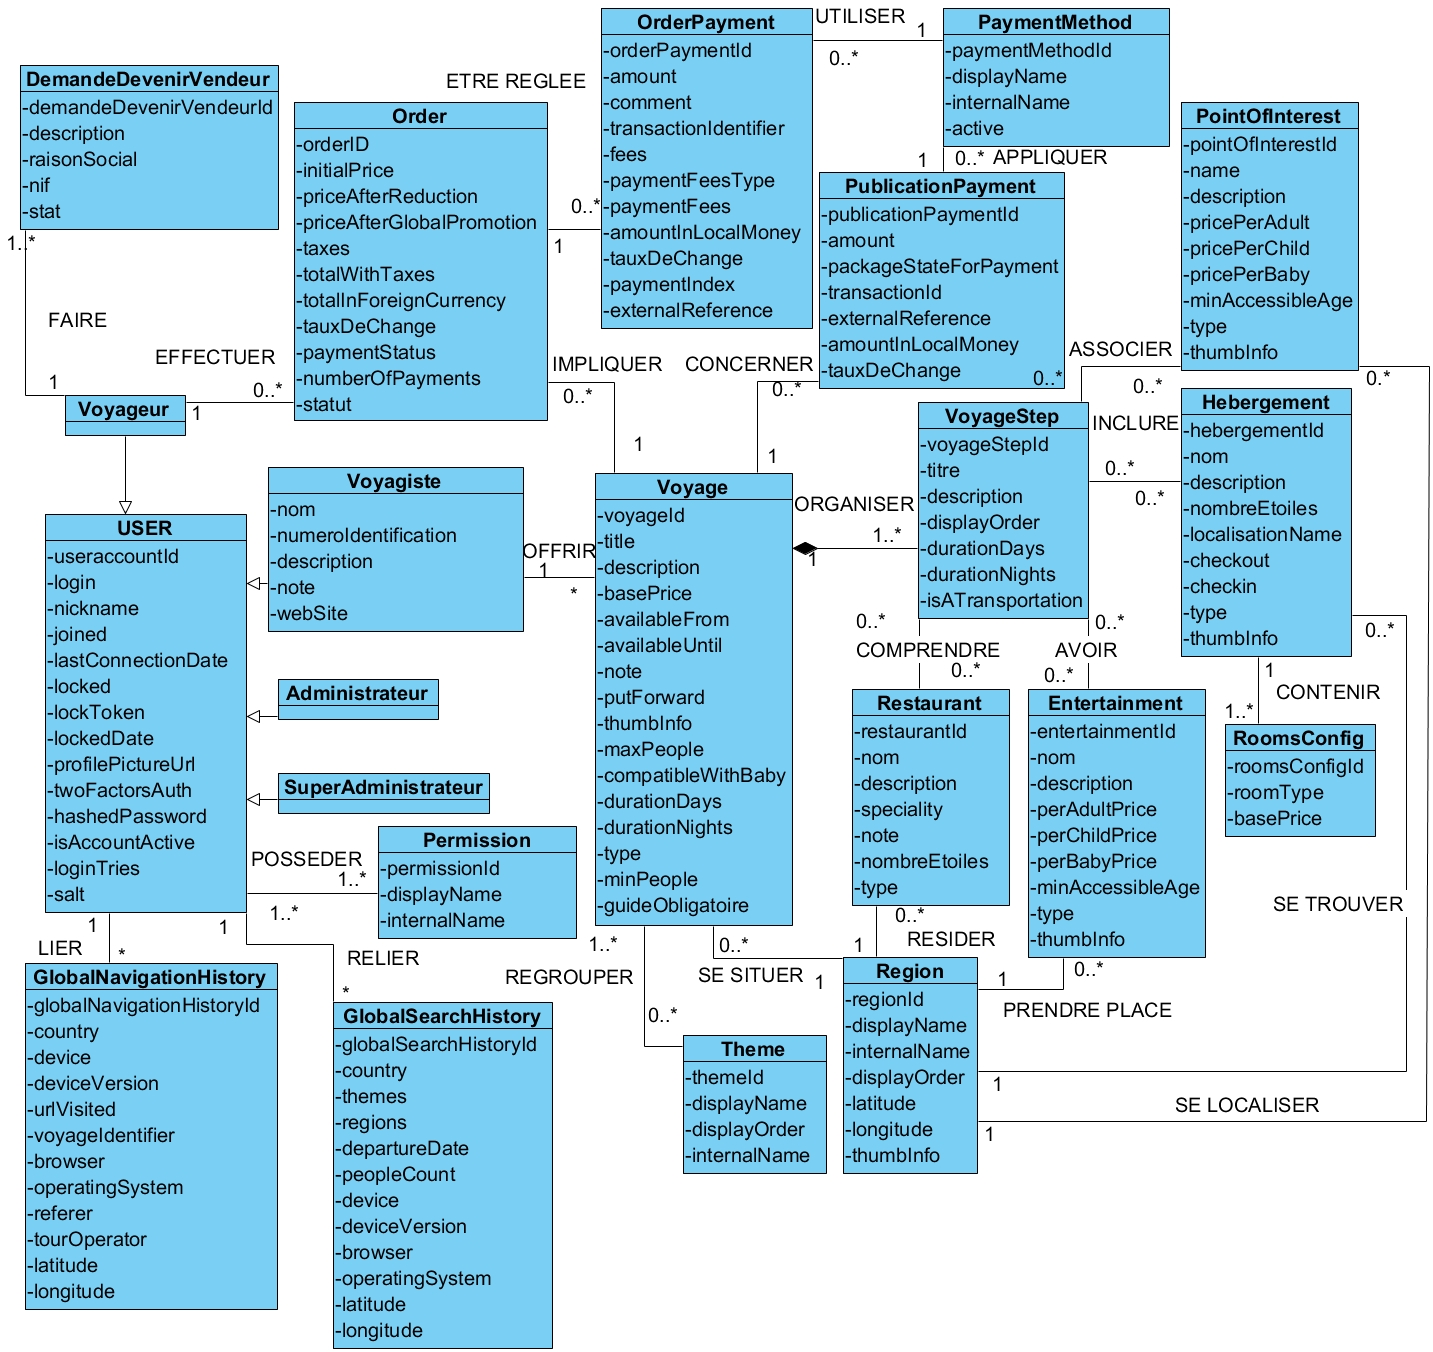
\includegraphics[width=\textwidth]{generalDC.jpg}
				\caption{Première vision du diagramme de classe}
				\label{fig:DCGlobal}
			\end{figure}
			\clearpage


			\section{Diagramme de classe de conception des différents sprints}
				\subsection{Principes de base}
				
				\hspace{15pt} Un diagramme de classes représente les entités d'un système et leurs relations, incluant leurs attributs et méthodes, avec pour objectif de modéliser la structure et le comportement du système de manière claire et compréhensible. Il est important car il facilite la conception, la communication et la documentation du système, aidant les développeurs et les parties prenantes à comprendre et à optimiser les interactions entre les différents composants du système.
				
				\subsection{Comment le représenter ?}
				
				\hspace{15pt} Pour représenter un diagramme de classes, identifiez les classes principales, leurs attributs et méthodes, établissez les relations entre elles, puis utilisez un outil de modélisation visuelle pour dessiner le diagramme de manière claire et structurée.

				Dans cette partie, nous allons examiner les diagrammes de classes de chaque sprint.

				\subsubsection{Diagramme de classe de conception pour le sprint 1}

				\hspace{15pt} La figure \ref{fig:sprint1} représente le diagramme de classes du sprint 1 qui se concentrent sur le développement du système d’authentification et l’inscription sur la plateforme.

			\begin{figure}[h]
				\centering
				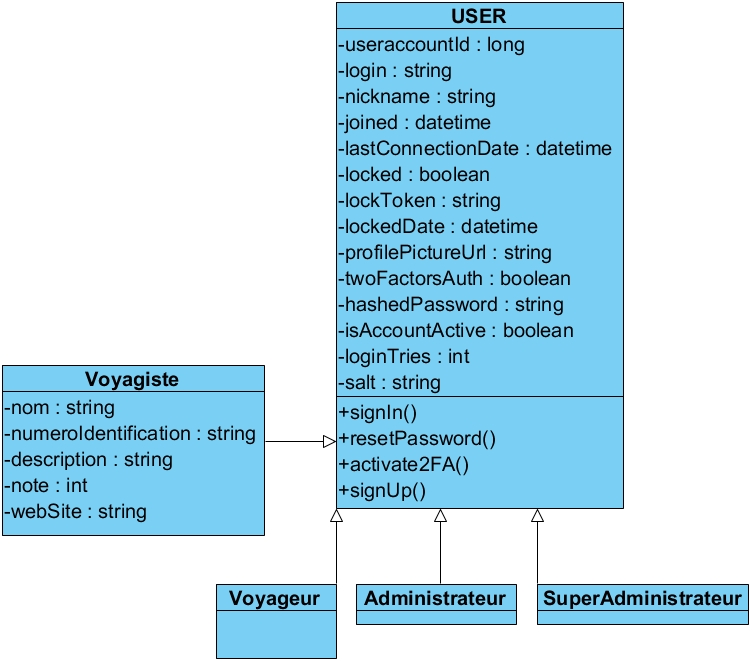
\includegraphics[width=0.6\textwidth]{sprint1.jpg}
				\caption{diagramme de classes du sprint 1}
				\label{fig:sprint1}
			\end{figure}
			\FloatBarrier

				\subsubsection{Diagramme de classe de conception pour le sprint 2}
				
			           \hspace{15pt} La figure \ref{fig:sprint2} représente le diagramme de classes du sprint 2 qui se concentrent sur la gestion des utilisateurs.

			\begin{figure}[h]
				\centering
				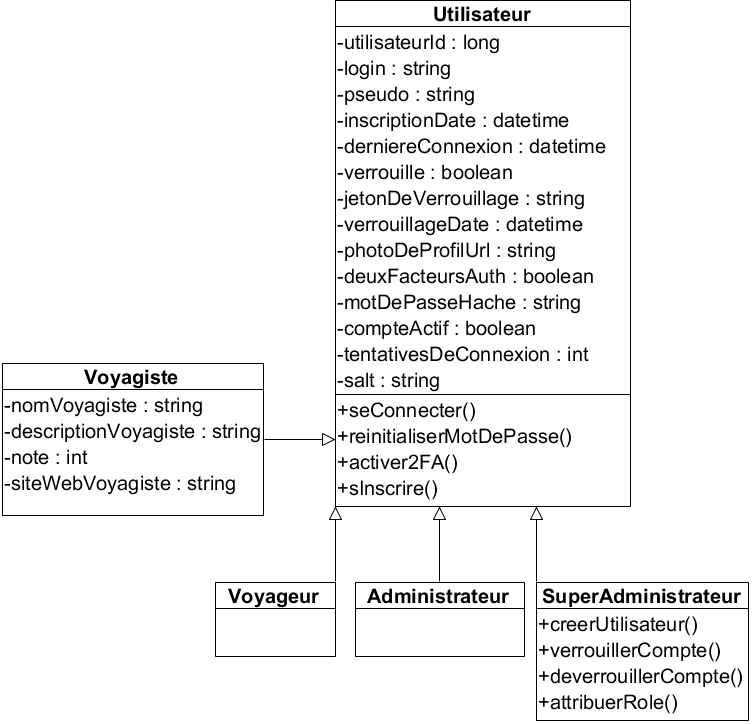
\includegraphics[width=0.6\textwidth]{sprint2.jpg}
				\caption{diagramme de classes du sprint 2}
				\label{fig:sprint2}
			\end{figure}
			\FloatBarrier

			\subsubsection{Diagramme de classe de conception pour le sprint 3}
				
			\hspace{15pt} La figure \ref{fig:sprint3} représente le diagramme de classes du sprint 3 qui se concentrent sur la gestion des rôles et
les permissions.


			\begin{figure}[h]
				\centering
				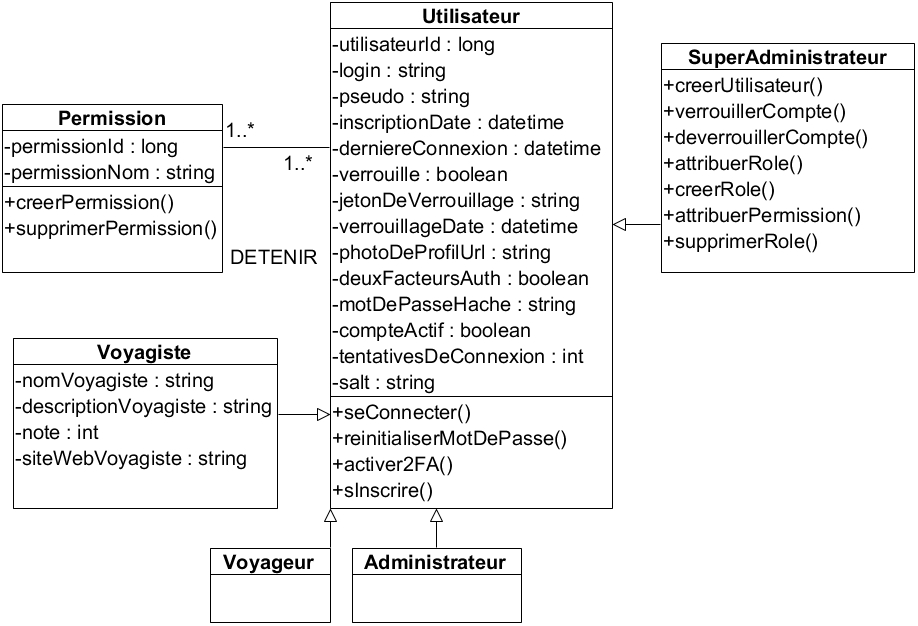
\includegraphics[width=0.9\textwidth]{sprint3.jpg}
				\caption{diagramme de classes du sprint 3}
				\label{fig:sprint3}
			\end{figure}
			\FloatBarrier


			\subsubsection{Diagramme de classe de conception pour le sprint 4}
				
			\hspace{15pt} La figure \ref{fig:sprint4} représente le diagramme de classes du sprint 4 qui se concentrent sur la gestion régions
et les thèmes.


			\begin{figure}[h]
				\centering
				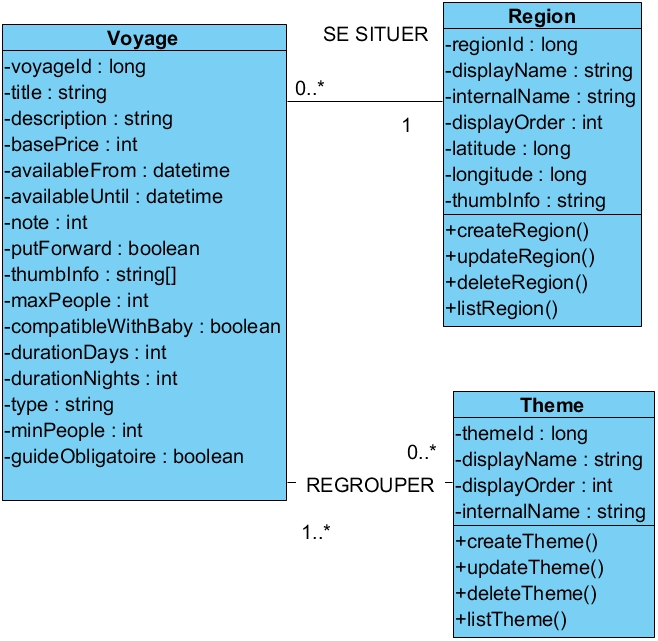
\includegraphics[width=0.6\textwidth]{sprint4.jpg}
				\caption{diagramme de classes du sprint 4}
				\label{fig:sprint4}
			\end{figure}
			\FloatBarrier

			\subsubsection{Diagramme de classe de conception pour le sprint 5}
				
			\hspace{15pt} La figure \ref{fig:sprint5} représente le diagramme de classes du sprint 5 qui se concentrent sur la gestion des circuits
et séjours.


			\begin{figure}[h]
				\centering
				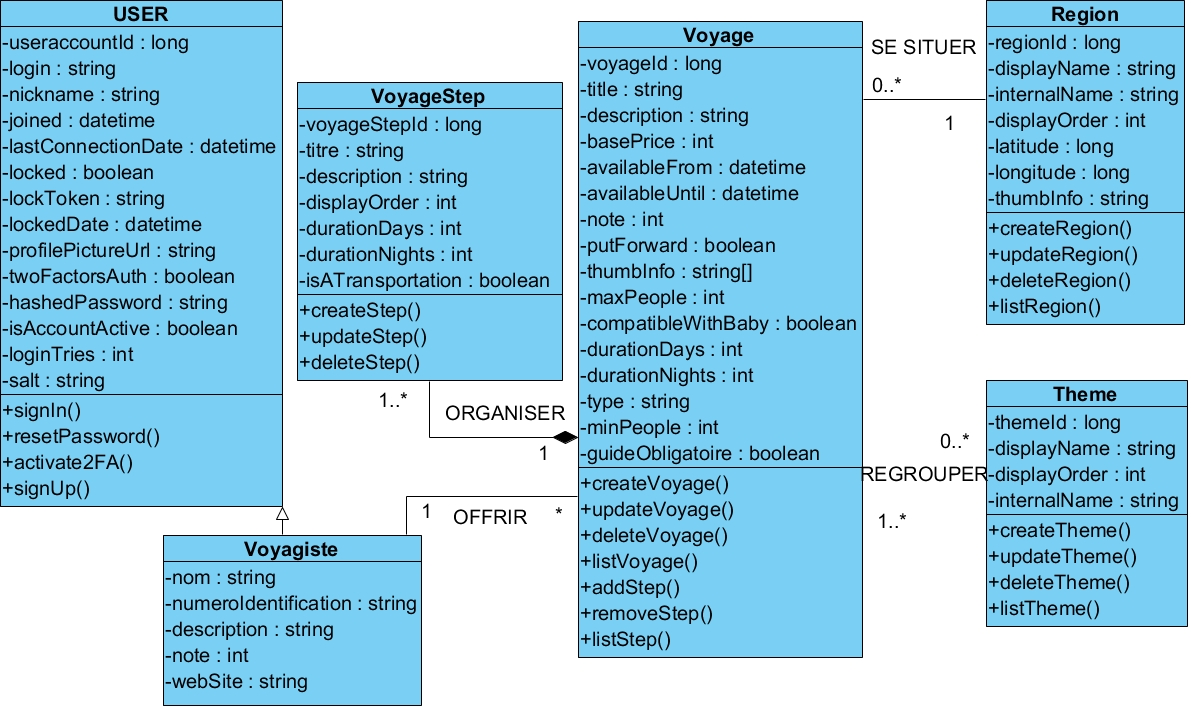
\includegraphics[width=0.9\textwidth]{sprint5.jpg}
				\caption{diagramme de classes du sprint 5}
				\label{fig:sprint5}
			\end{figure}
			\FloatBarrier


			\subsubsection{Diagramme de classe de conception pour le sprint 6}
				
			\hspace{15pt} La figure \ref{fig:sprint6} représente le diagramme de classes du sprint 6 qui se concentrent sur la Recherche des
voyages.


			\begin{figure}[h]
				\centering
				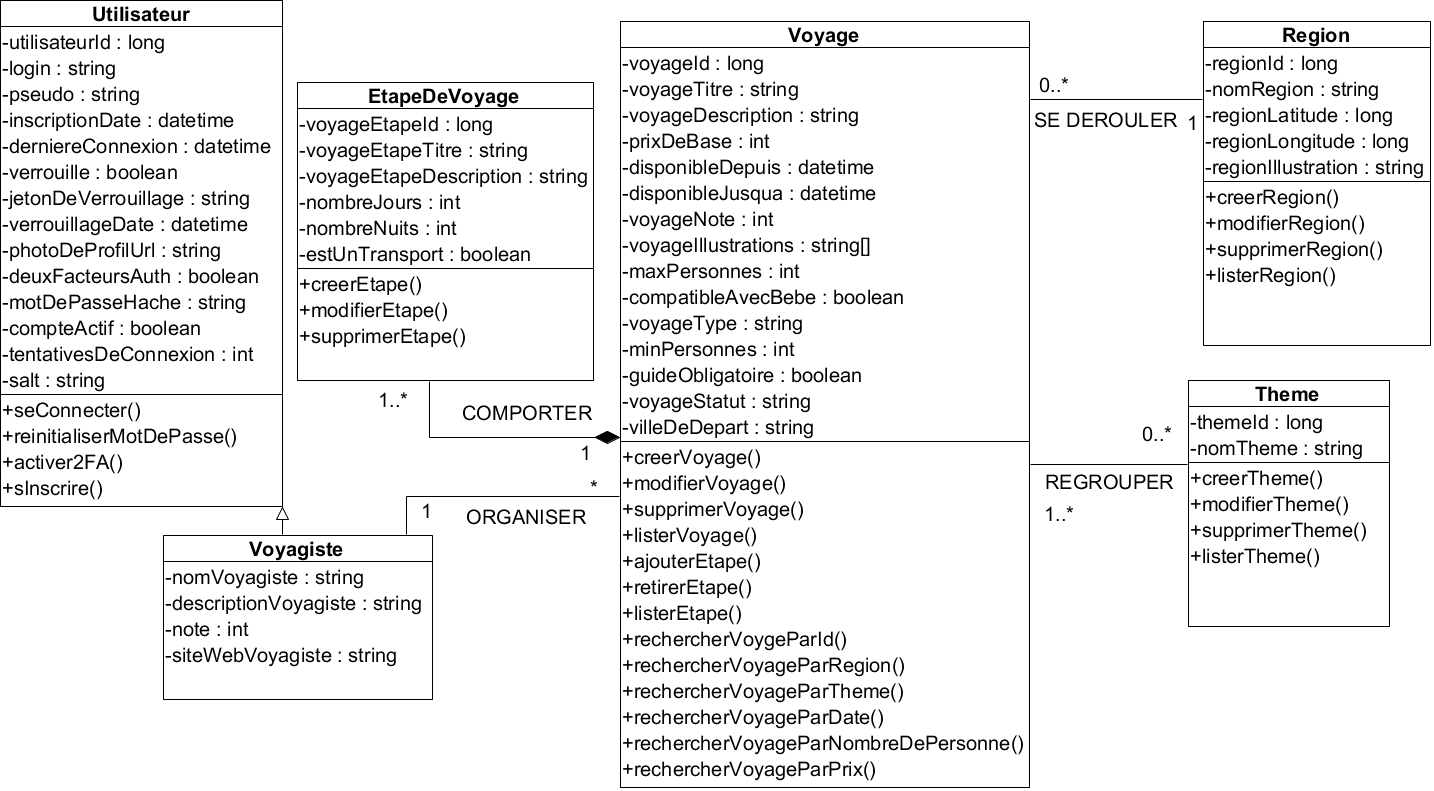
\includegraphics[width=\textwidth]{sprint6.jpg}
				\caption{diagramme de classes du sprint 6}
				\label{fig:sprint6}
			\end{figure}
			\FloatBarrier

			\subsubsection{Diagramme de classe de conception pour le sprint 7}
				
			\hspace{15pt} La figure \ref{fig:sprint7} représente le diagramme de classes du sprint 7 qui se concentrent sur la Réservation des voy-
ages.


			\begin{figure}[h]
				\centering
				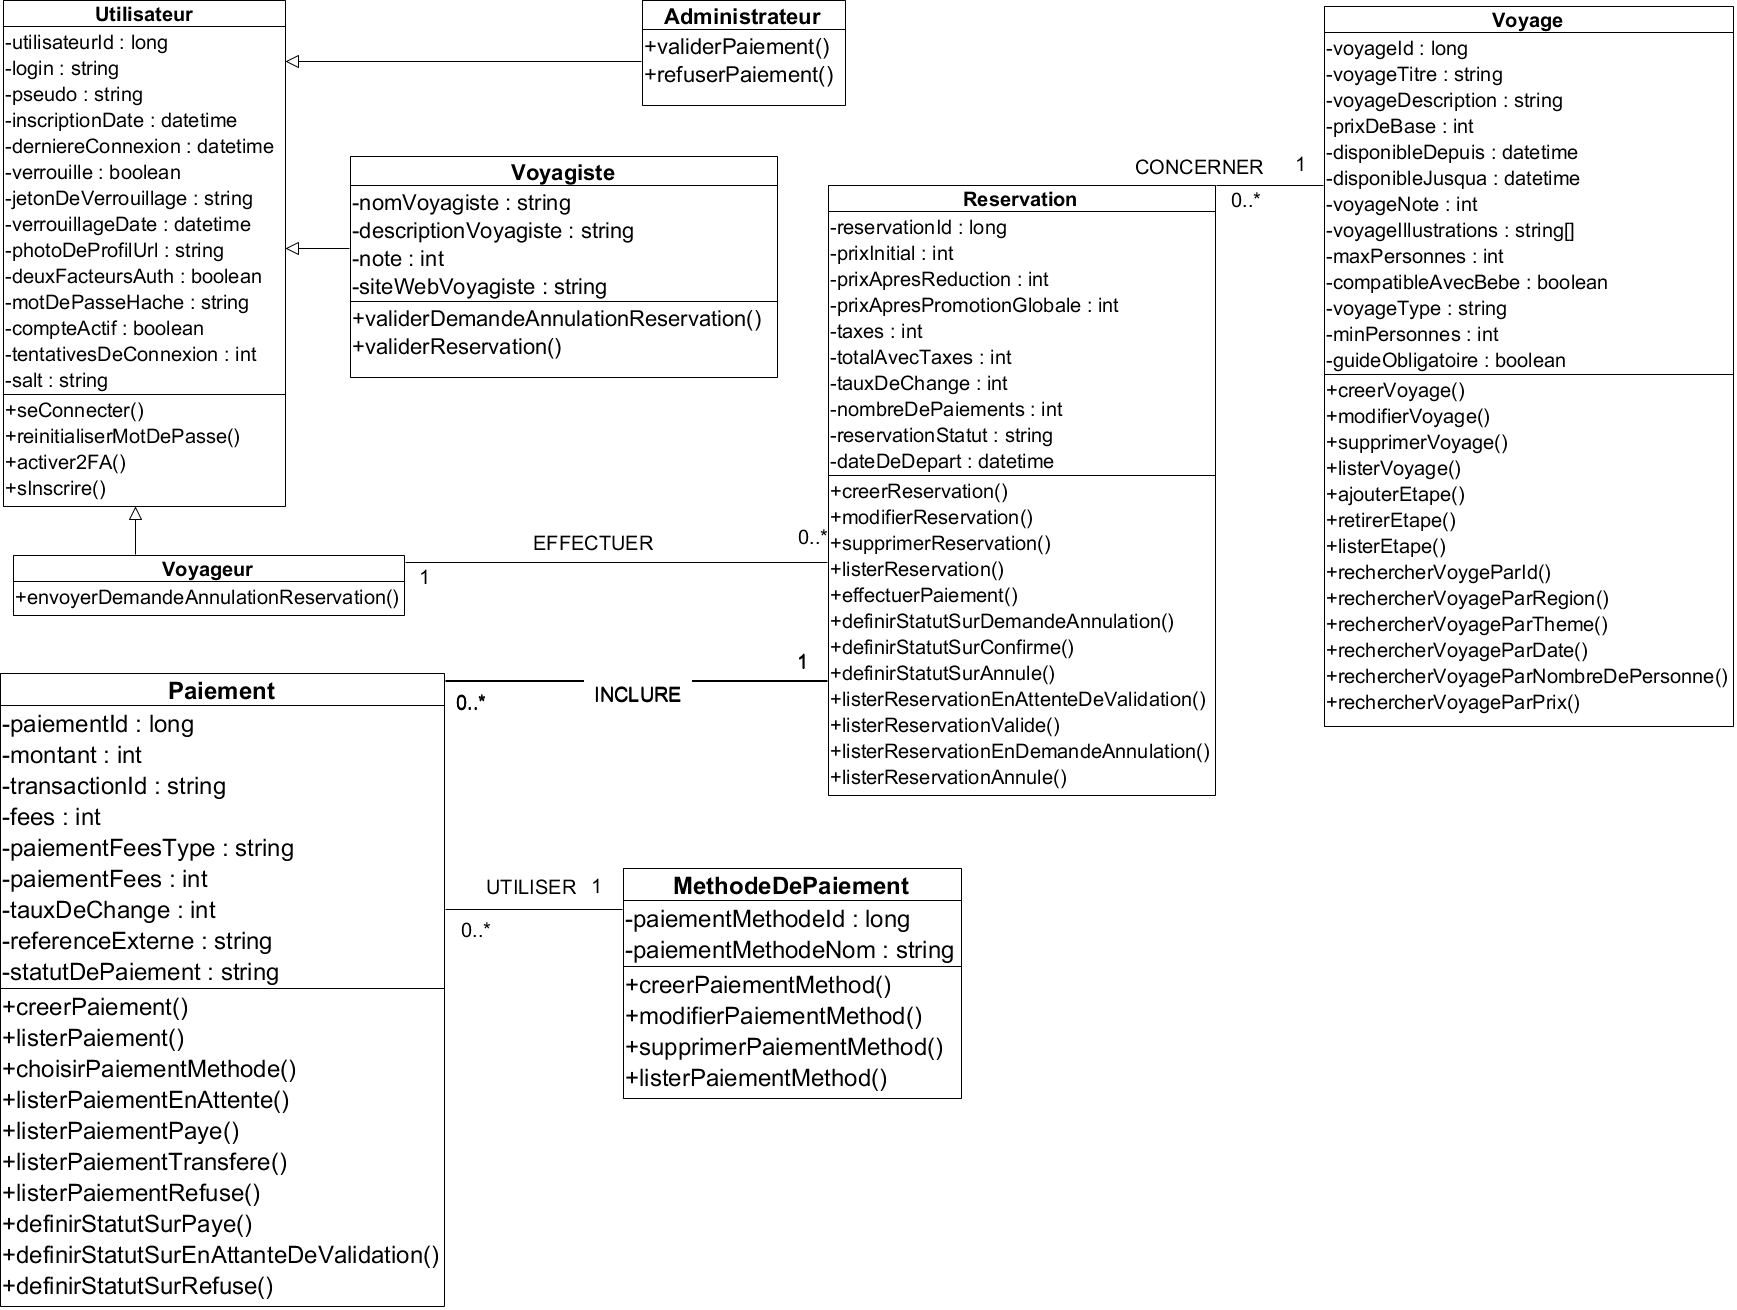
\includegraphics[width=\textwidth]{sprint7.jpg}
				\caption{diagramme de classes du sprint 7}
				\label{fig:sprint7}
			\end{figure}
			\FloatBarrier


			\subsubsection{Diagramme de classe de conception pour le sprint 8}
				
			\hspace{15pt} La figure \ref{fig:sprint8} représente le diagramme de classes du sprint 8 qui se concentrent sur le Paiement des réservations.


			\begin{figure}[h]
				\centering
				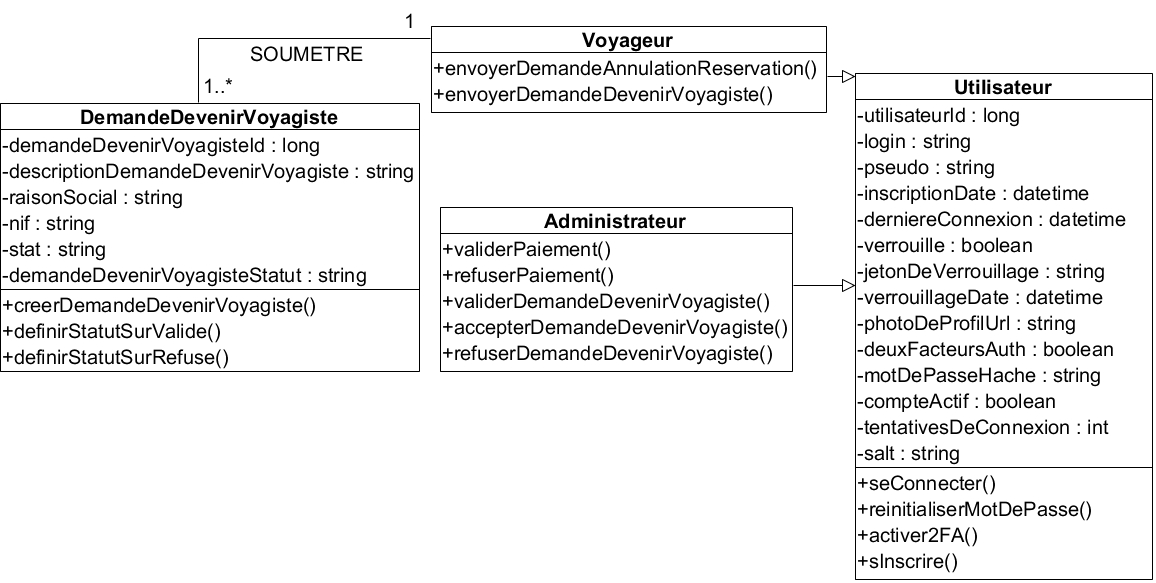
\includegraphics[width=\textwidth]{sprint8.jpg}
				\caption{diagramme de classes du sprint 8}
				\label{fig:sprint8}
			\end{figure}
			\FloatBarrier


			\subsubsection{Diagramme de classe de conception pour le sprint 9}
				
			\hspace{15pt} La figure \ref{fig:sprint9} représente le diagramme de classes du sprint 9 qui se concentrent sur les demandes d’annulation des réservations.


			\begin{figure}[h]
				\centering
				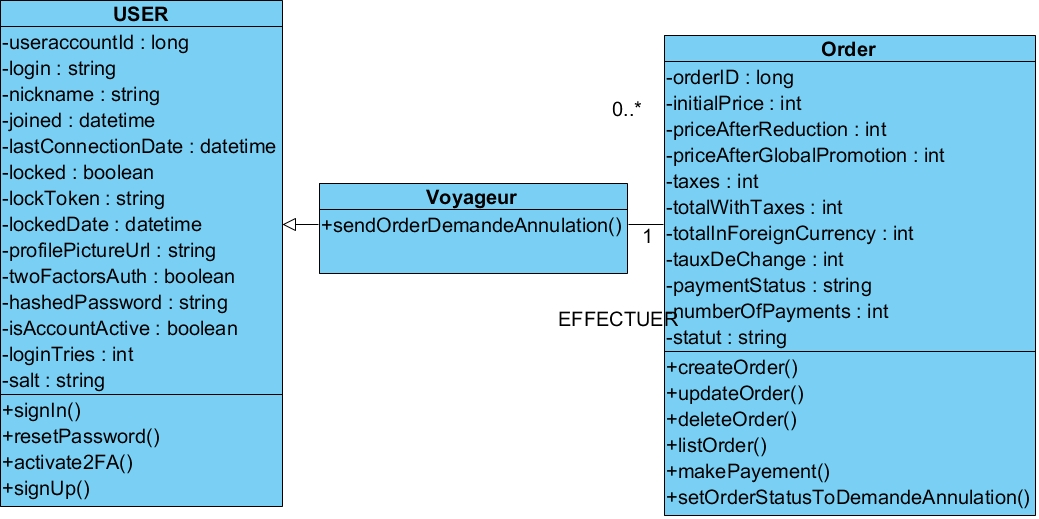
\includegraphics[width=\textwidth]{sprint9.jpg}
				\caption{diagramme de classes du sprint 9}
				\label{fig:sprint9}
			\end{figure}
			\FloatBarrier

			\subsubsection{Diagramme de classe de conception pour le sprint 10}
				
			\hspace{15pt} La figure \ref{fig:sprint10} représente le diagramme de classes du sprint 10 qui se concentrent sur la gestion des réservations.


			\begin{figure}[h]
				\centering
				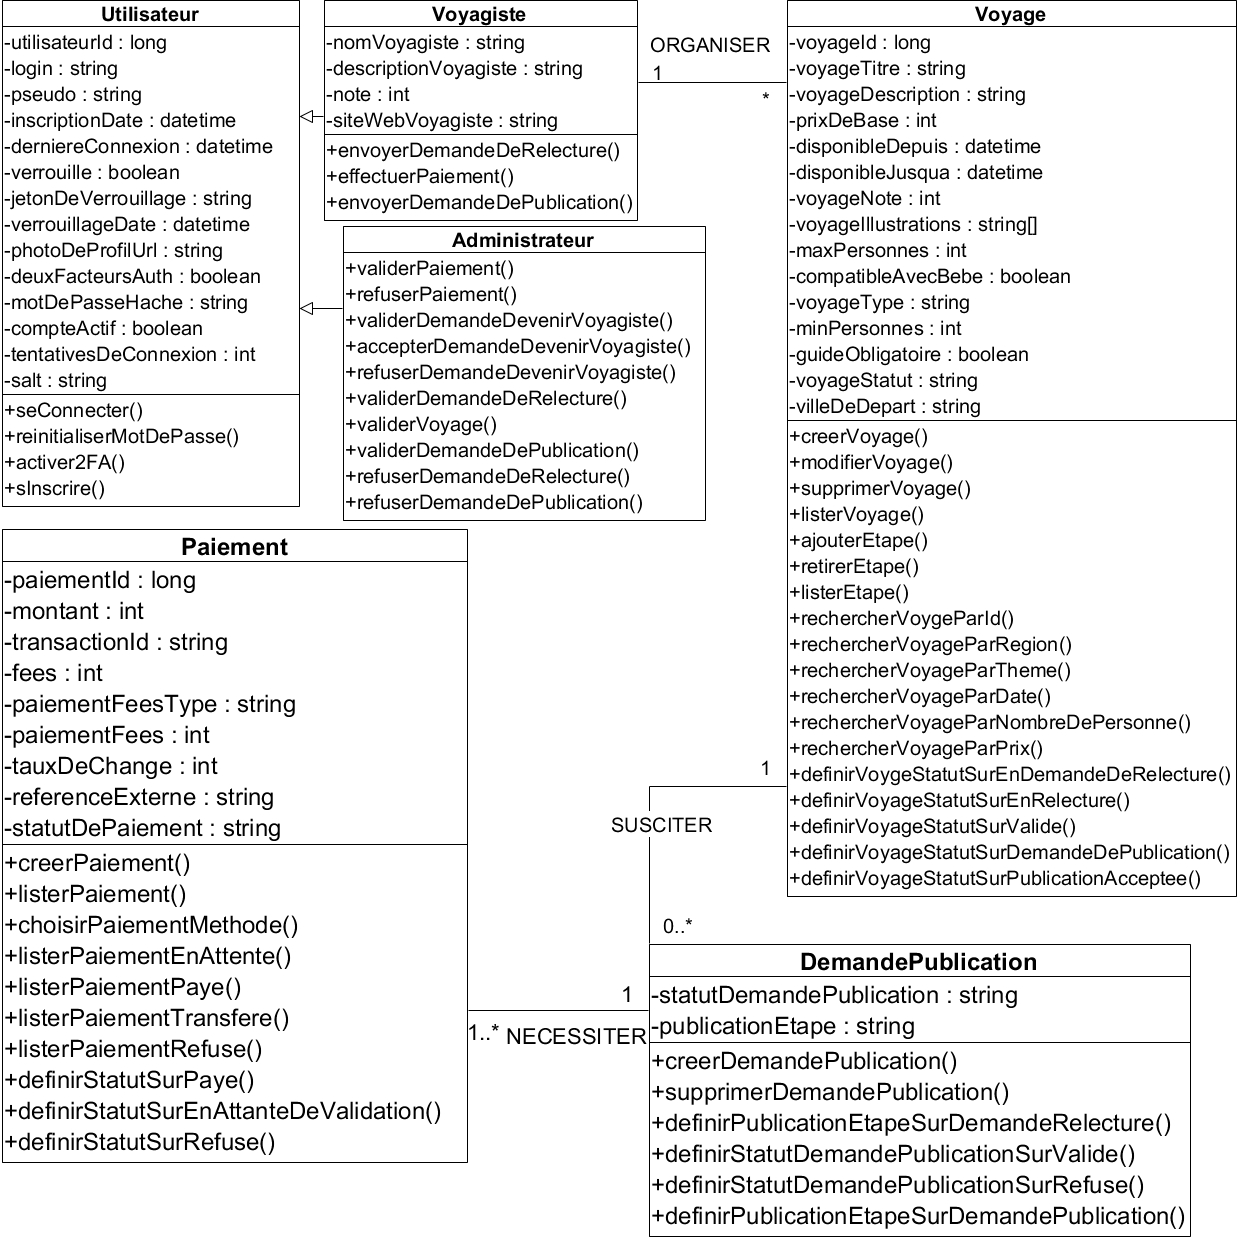
\includegraphics[width=\textwidth]{sprint10.jpg}
				\caption{diagramme de classes du sprint 10}
				\label{fig:sprint10}
			\end{figure}
			\FloatBarrier

			\subsubsection{Diagramme de classe de conception pour le sprint 11}
				
			\hspace{15pt} La figure \ref{fig:sprint11} représente le diagramme de classes du sprint 11 qui se concentrent sur la suivi des paiements.


			\begin{figure}[h]
				\centering
				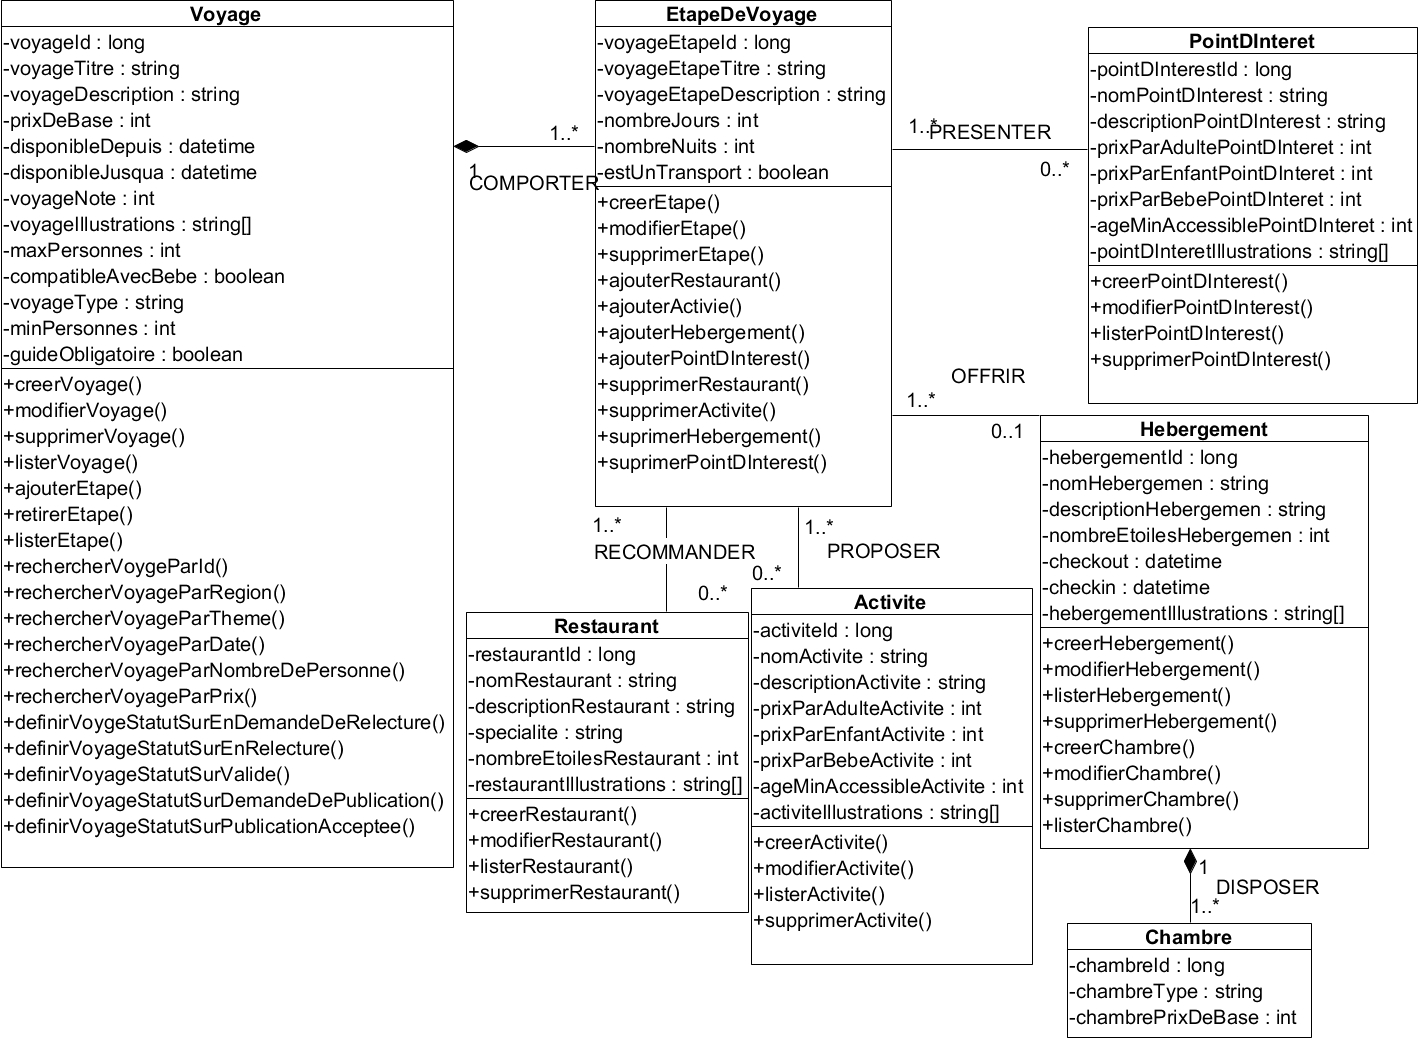
\includegraphics[width=\textwidth]{sprint11.jpg}
				\caption{diagramme de classes du sprint 11}
				\label{fig:sprint11}
			\end{figure}
			\FloatBarrier


			\subsubsection{Diagramme de classe de conception pour le sprint 12}
				
			\hspace{15pt} La figure \ref{fig:sprint12} représente le diagramme de classes du sprint 12 qui se concentrent sur le suivi des statistiques des opérations sur la plateforme.


			\begin{figure}[h]
				\centering
				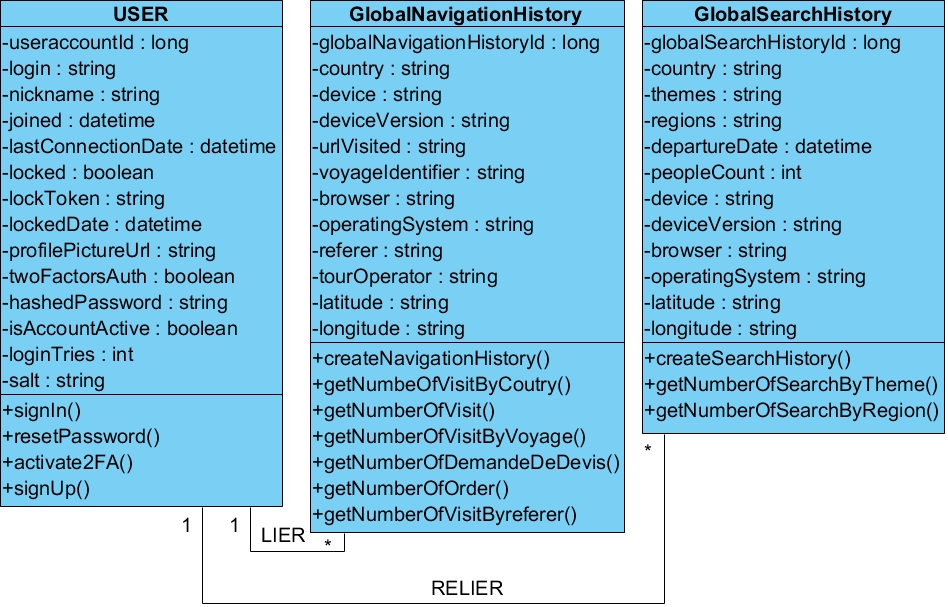
\includegraphics[width=0.7\textwidth]{sprint12.jpg}
				\caption{diagramme de classes du sprint 12}
				\label{fig:sprint12}
			\end{figure}
			\FloatBarrier

			\subsubsection{Diagramme de classe de conception pour le sprint 13}
				
			\hspace{15pt} La figure \ref{fig:sprint13} représente le diagramme de classes du sprint 13 qui se concentrent sur le suivi des statistiques des circuits et séjours.


			\begin{figure}[h]
				\centering
				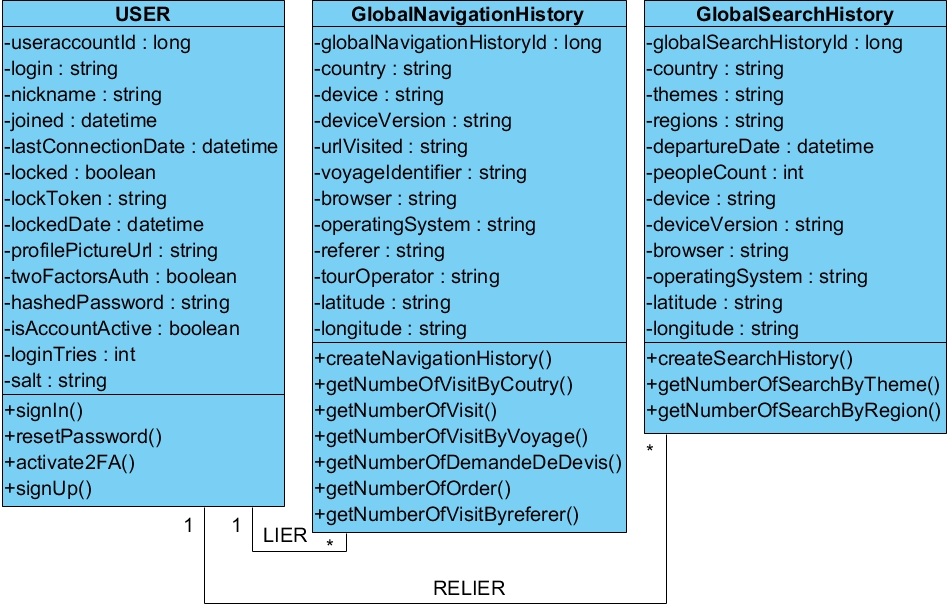
\includegraphics[width=0.7\textwidth]{sprint13.jpg}
				\caption{diagramme de classes du sprint 13}
				\label{fig:sprint13}
			\end{figure}
			\FloatBarrier


			\subsubsection{Diagramme de classe de conception pour le sprint 14}
				
			\hspace{15pt} La figure \ref{fig:sprint14} représente le diagramme de classes du sprint 14 qui se concentrent sur la gestion des demandes de devenir voyagiste sur la plateforme.


			\begin{figure}[h]
				\centering
				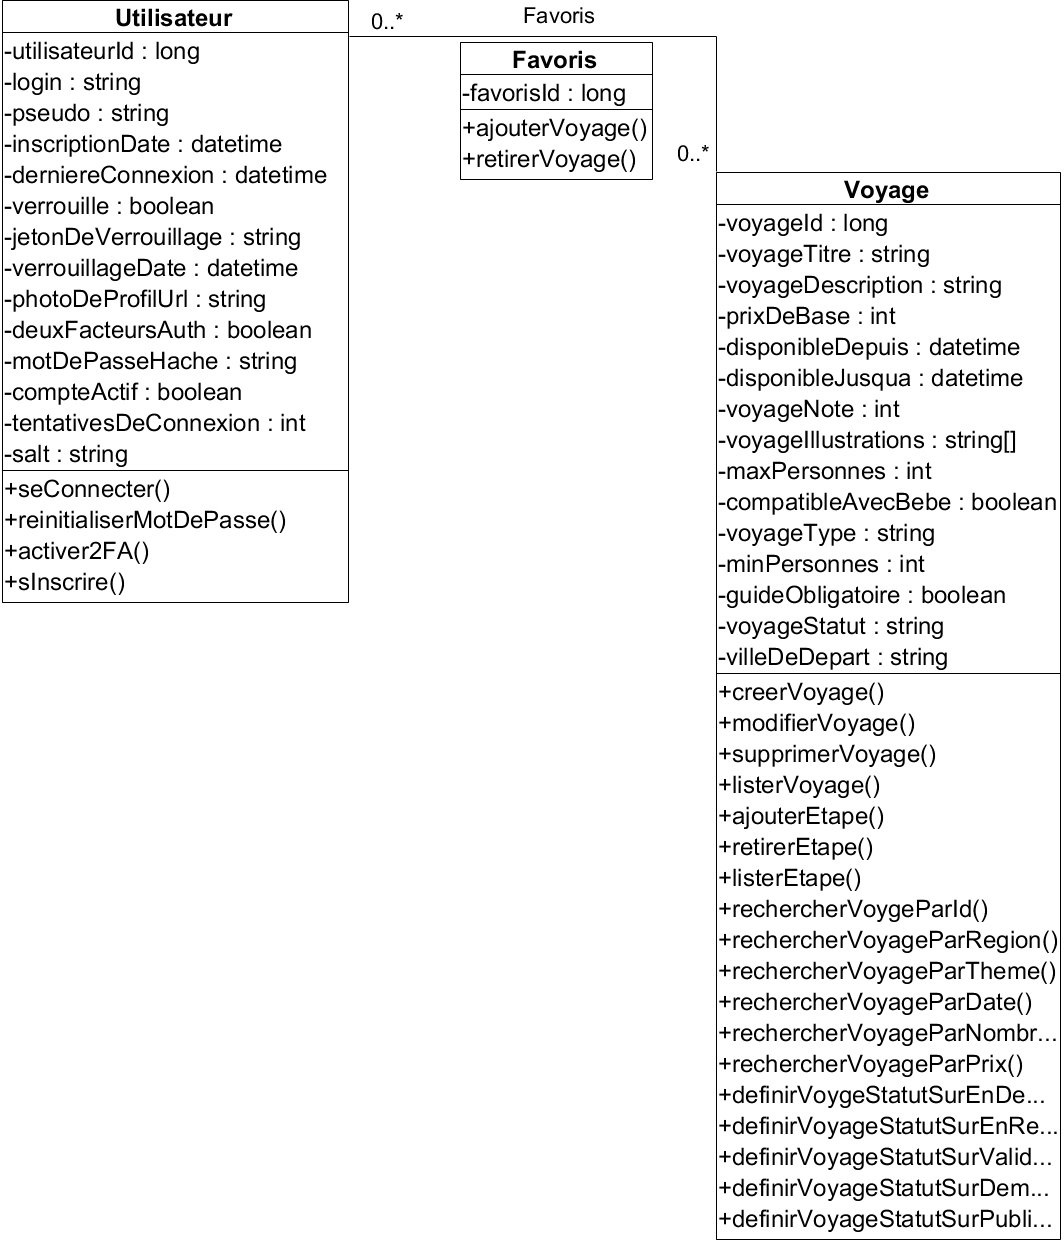
\includegraphics[width=0.9\textwidth]{sprint14.jpg}
				\caption{diagramme de classes du sprint 14}
				\label{fig:sprint14}
			\end{figure}
			\FloatBarrier


			\subsubsection{Diagramme de classe de conception pour le sprint 15}
				
			\hspace{15pt} La figure \ref{fig:sprint15} représente le diagramme de classes du sprint 15 qui se concentrent sur la gestion des demandes de validation des circuits et séjours.


			\begin{figure}[h]
				\centering
				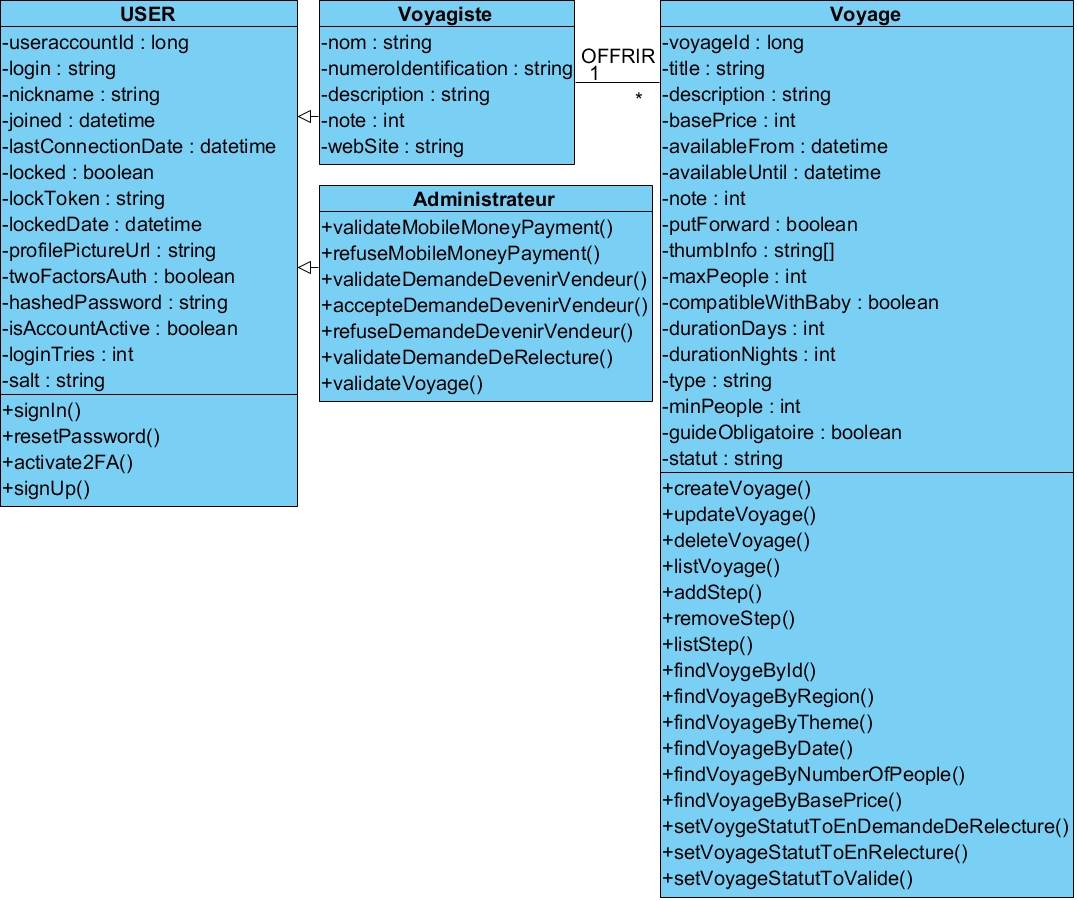
\includegraphics[width=0.9\textwidth]{sprint15.jpg}
				\caption{diagramme de classes du sprint 15}
				\label{fig:sprint15}
			\end{figure}
			\FloatBarrier

			\subsubsection{Diagramme de classe de conception pour le sprint 16}
				
			\hspace{15pt} La figure \ref{fig:sprint16} représente le diagramme de classes du sprint 16 qui se concentrent sur la gestion des demandes de publication des circuits et séjours.


			\begin{figure}[h]
				\centering
				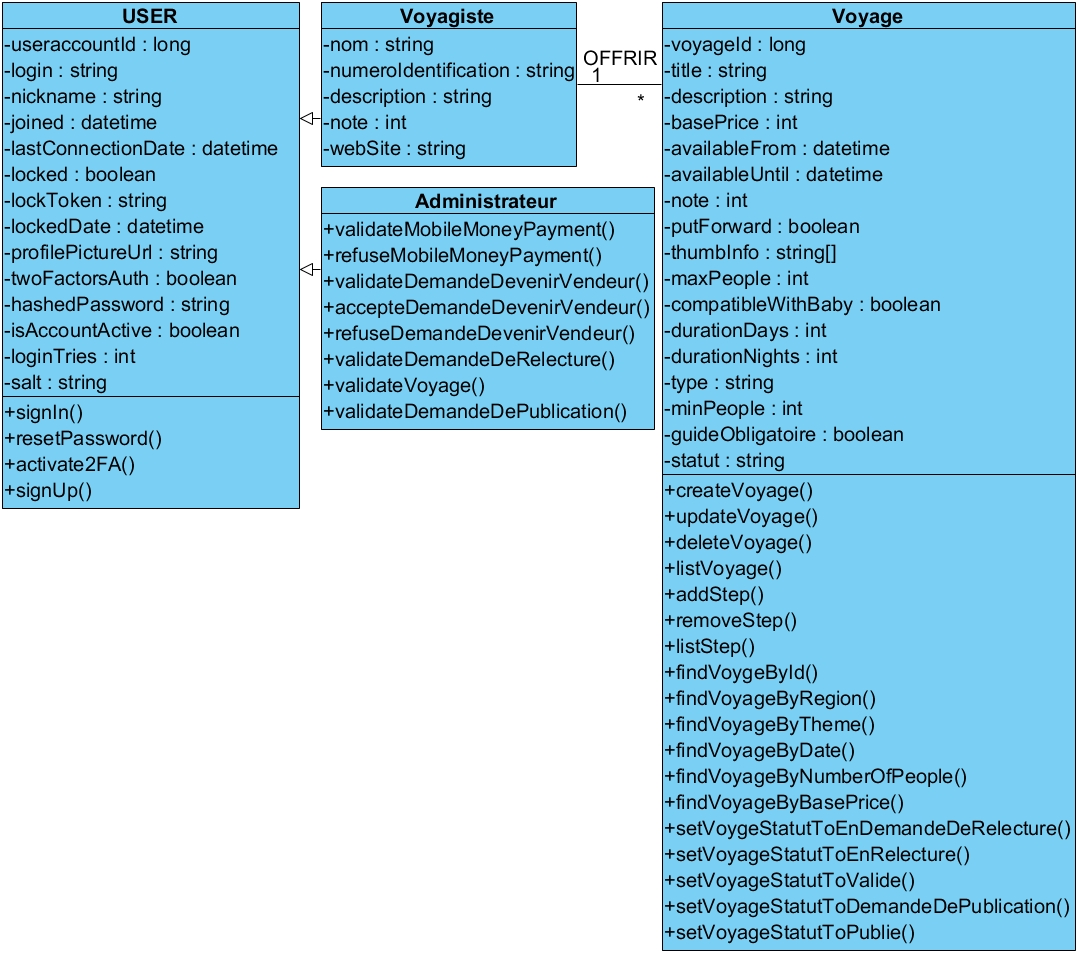
\includegraphics[width=0.9\textwidth]{sprint16.jpg}
				\caption{diagramme de classes du sprint 16}
				\label{fig:sprint16}
			\end{figure}
			\FloatBarrier


			\subsubsection{Diagramme de classe de conception pour le sprint 17}
				
			\hspace{15pt} La figure \ref{fig:sprint17} représente le diagramme de classes du sprint 17 qui se concentrent sur la gestion des hébergements, restaurations, activités et points d’intérêtdes des circuits et séjours.


			\begin{figure}[h]
				\centering
				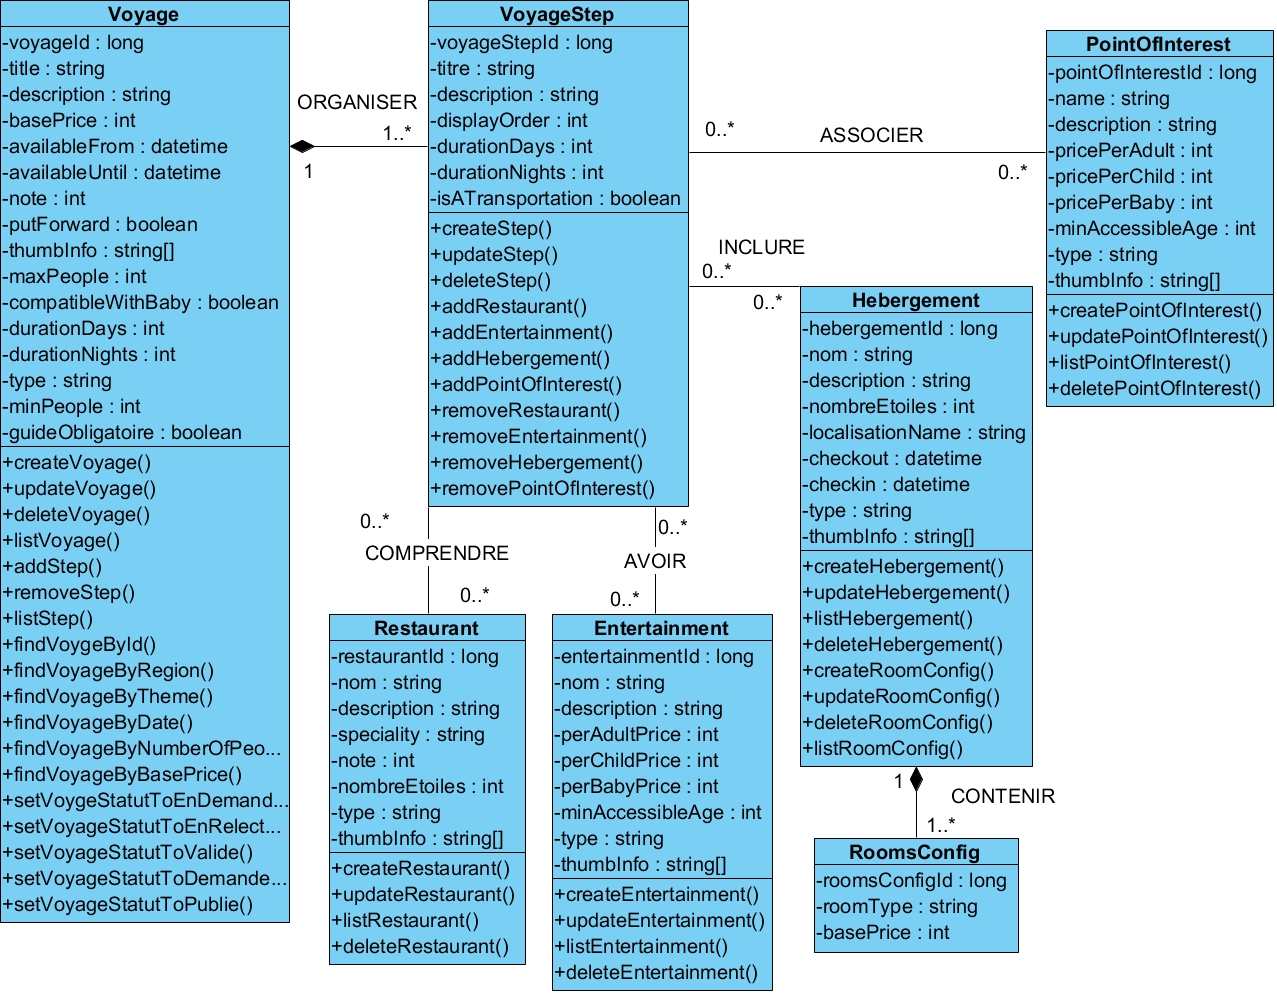
\includegraphics[width=\textwidth]{sprint17.jpg}
				\caption{diagramme de classes du sprint 17}
				\label{fig:sprint17}
			\end{figure}
			\FloatBarrier

			\subsubsection{Diagramme de classe de conception pour le sprint 18}
				
			\hspace{15pt} La figure \ref{fig:sprint18} représente le diagramme de classes du sprint 18 qui se concentrent sur l' envoye des demandes de validation des circuits et séjours.


			\begin{figure}[h]
				\centering
				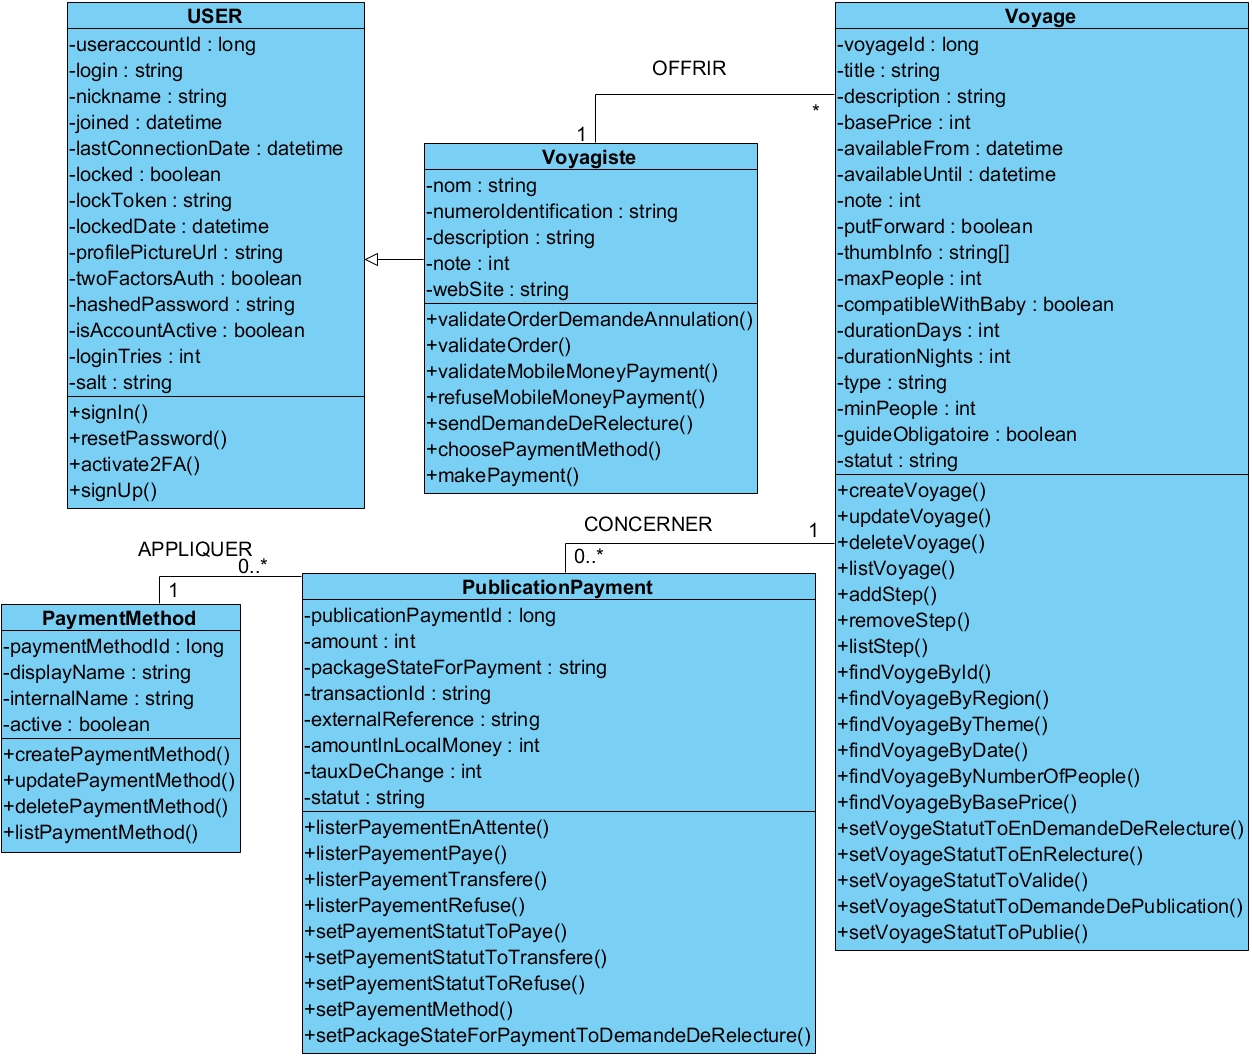
\includegraphics[width=0.9\textwidth]{sprint18.jpg}
				\caption{diagramme de classes du sprint 18}
				\label{fig:sprint18}
			\end{figure}
			\FloatBarrier

			\subsubsection{Diagramme de classe de conception pour le sprint 19}
				
			\hspace{15pt} La figure \ref{fig:sprint19} représente le diagramme de classes du sprint 19 qui se concentrent sur l' envoye des demandes de publication des circuits et séjours.


			\begin{figure}[h]
				\centering
				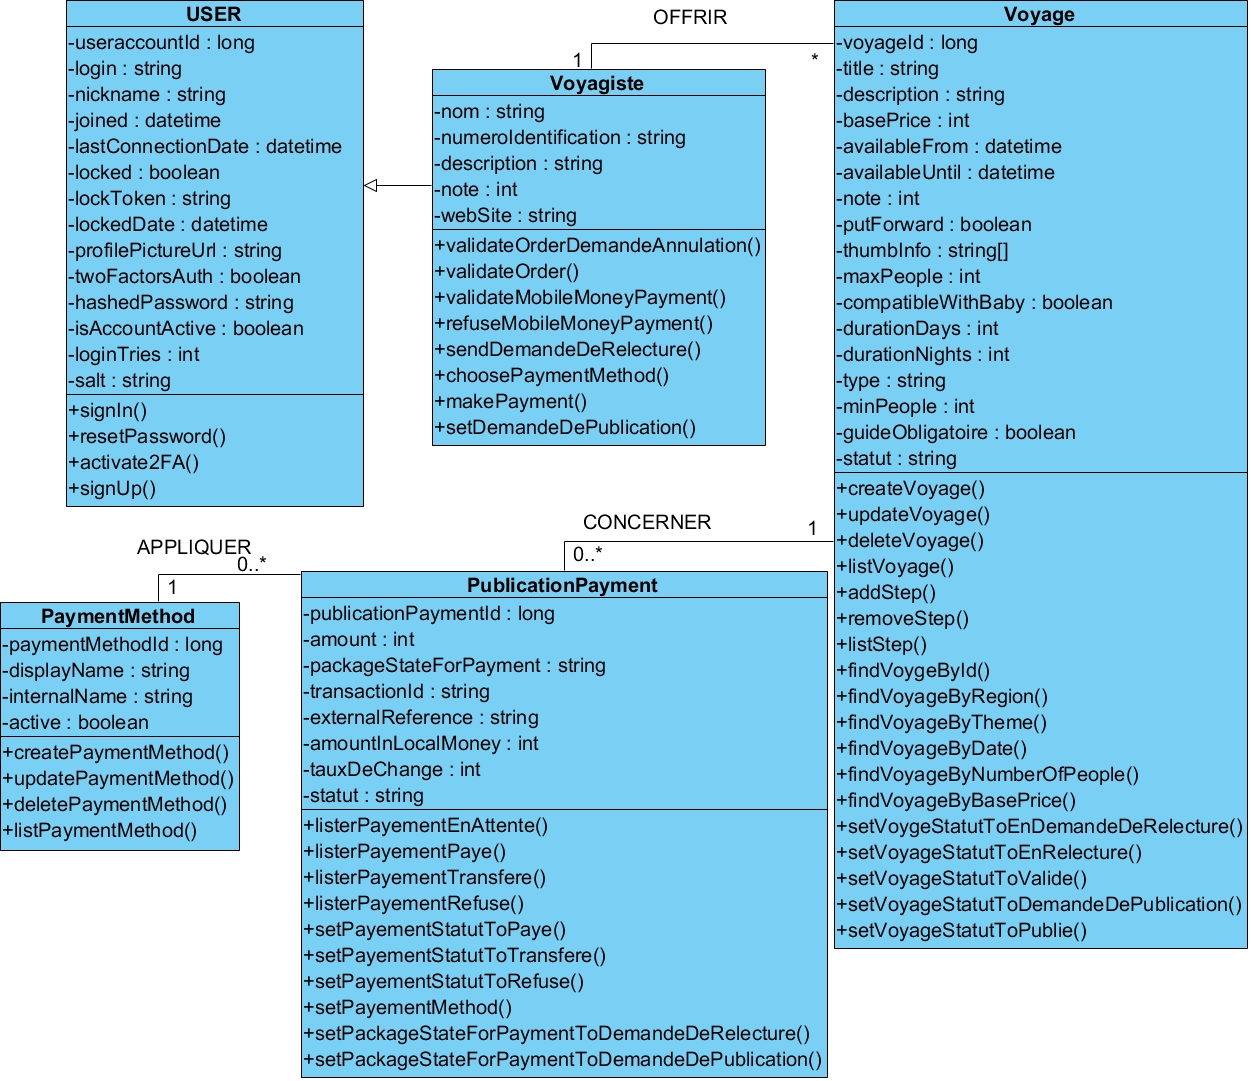
\includegraphics[width=0.9\textwidth]{sprint19.jpg}
				\caption{diagramme de classes du sprint 19}
				\label{fig:sprint19}
			\end{figure}
			\FloatBarrier

			\subsubsection{Diagramme de classe de conception pour le sprint 20}
				
			\hspace{15pt} La figure \ref{fig:sprint20} représente le diagramme de classes du sprint 20 qui se concentrent sur l' envoye des demandes de validation des circuits et séjours.


			\begin{figure}[h]
				\centering
				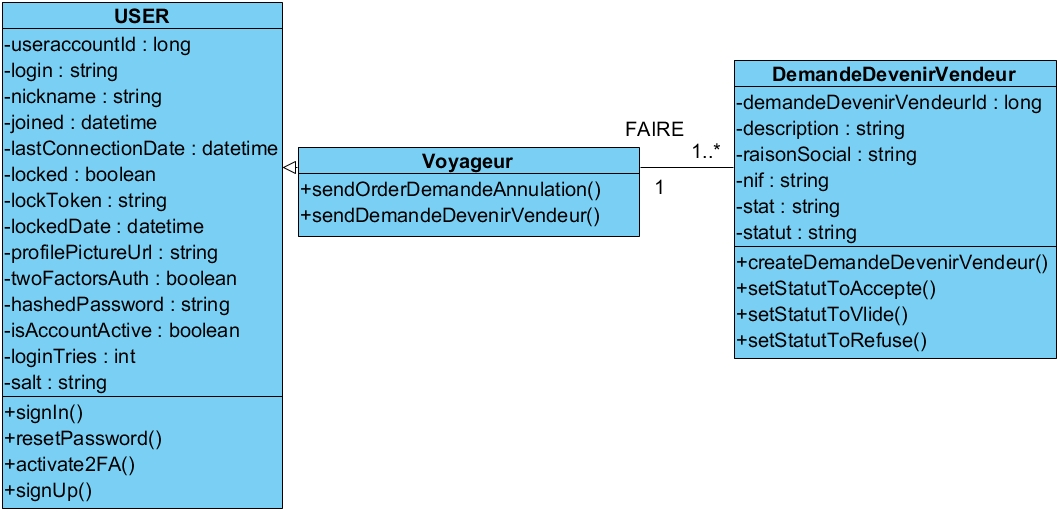
\includegraphics[width=0.9\textwidth]{sprint20.jpg}
				\caption{diagramme de classes du sprint 20}
				\label{fig:sprint20}
			\end{figure}
			\FloatBarrier


			\section{Diagramme de classe de conception globale}
			Le diagramme de classe de conception globale illustre une vue d'ensemble de la structure du système entier pour guider sa conception et son développement.
				
			\hspace{15pt} La figure \ref{fig:DCFinal} représente le diagramme de classe de conception globale du projet Handeha Voyage.

			\begin{figure}[h]
				\centering
				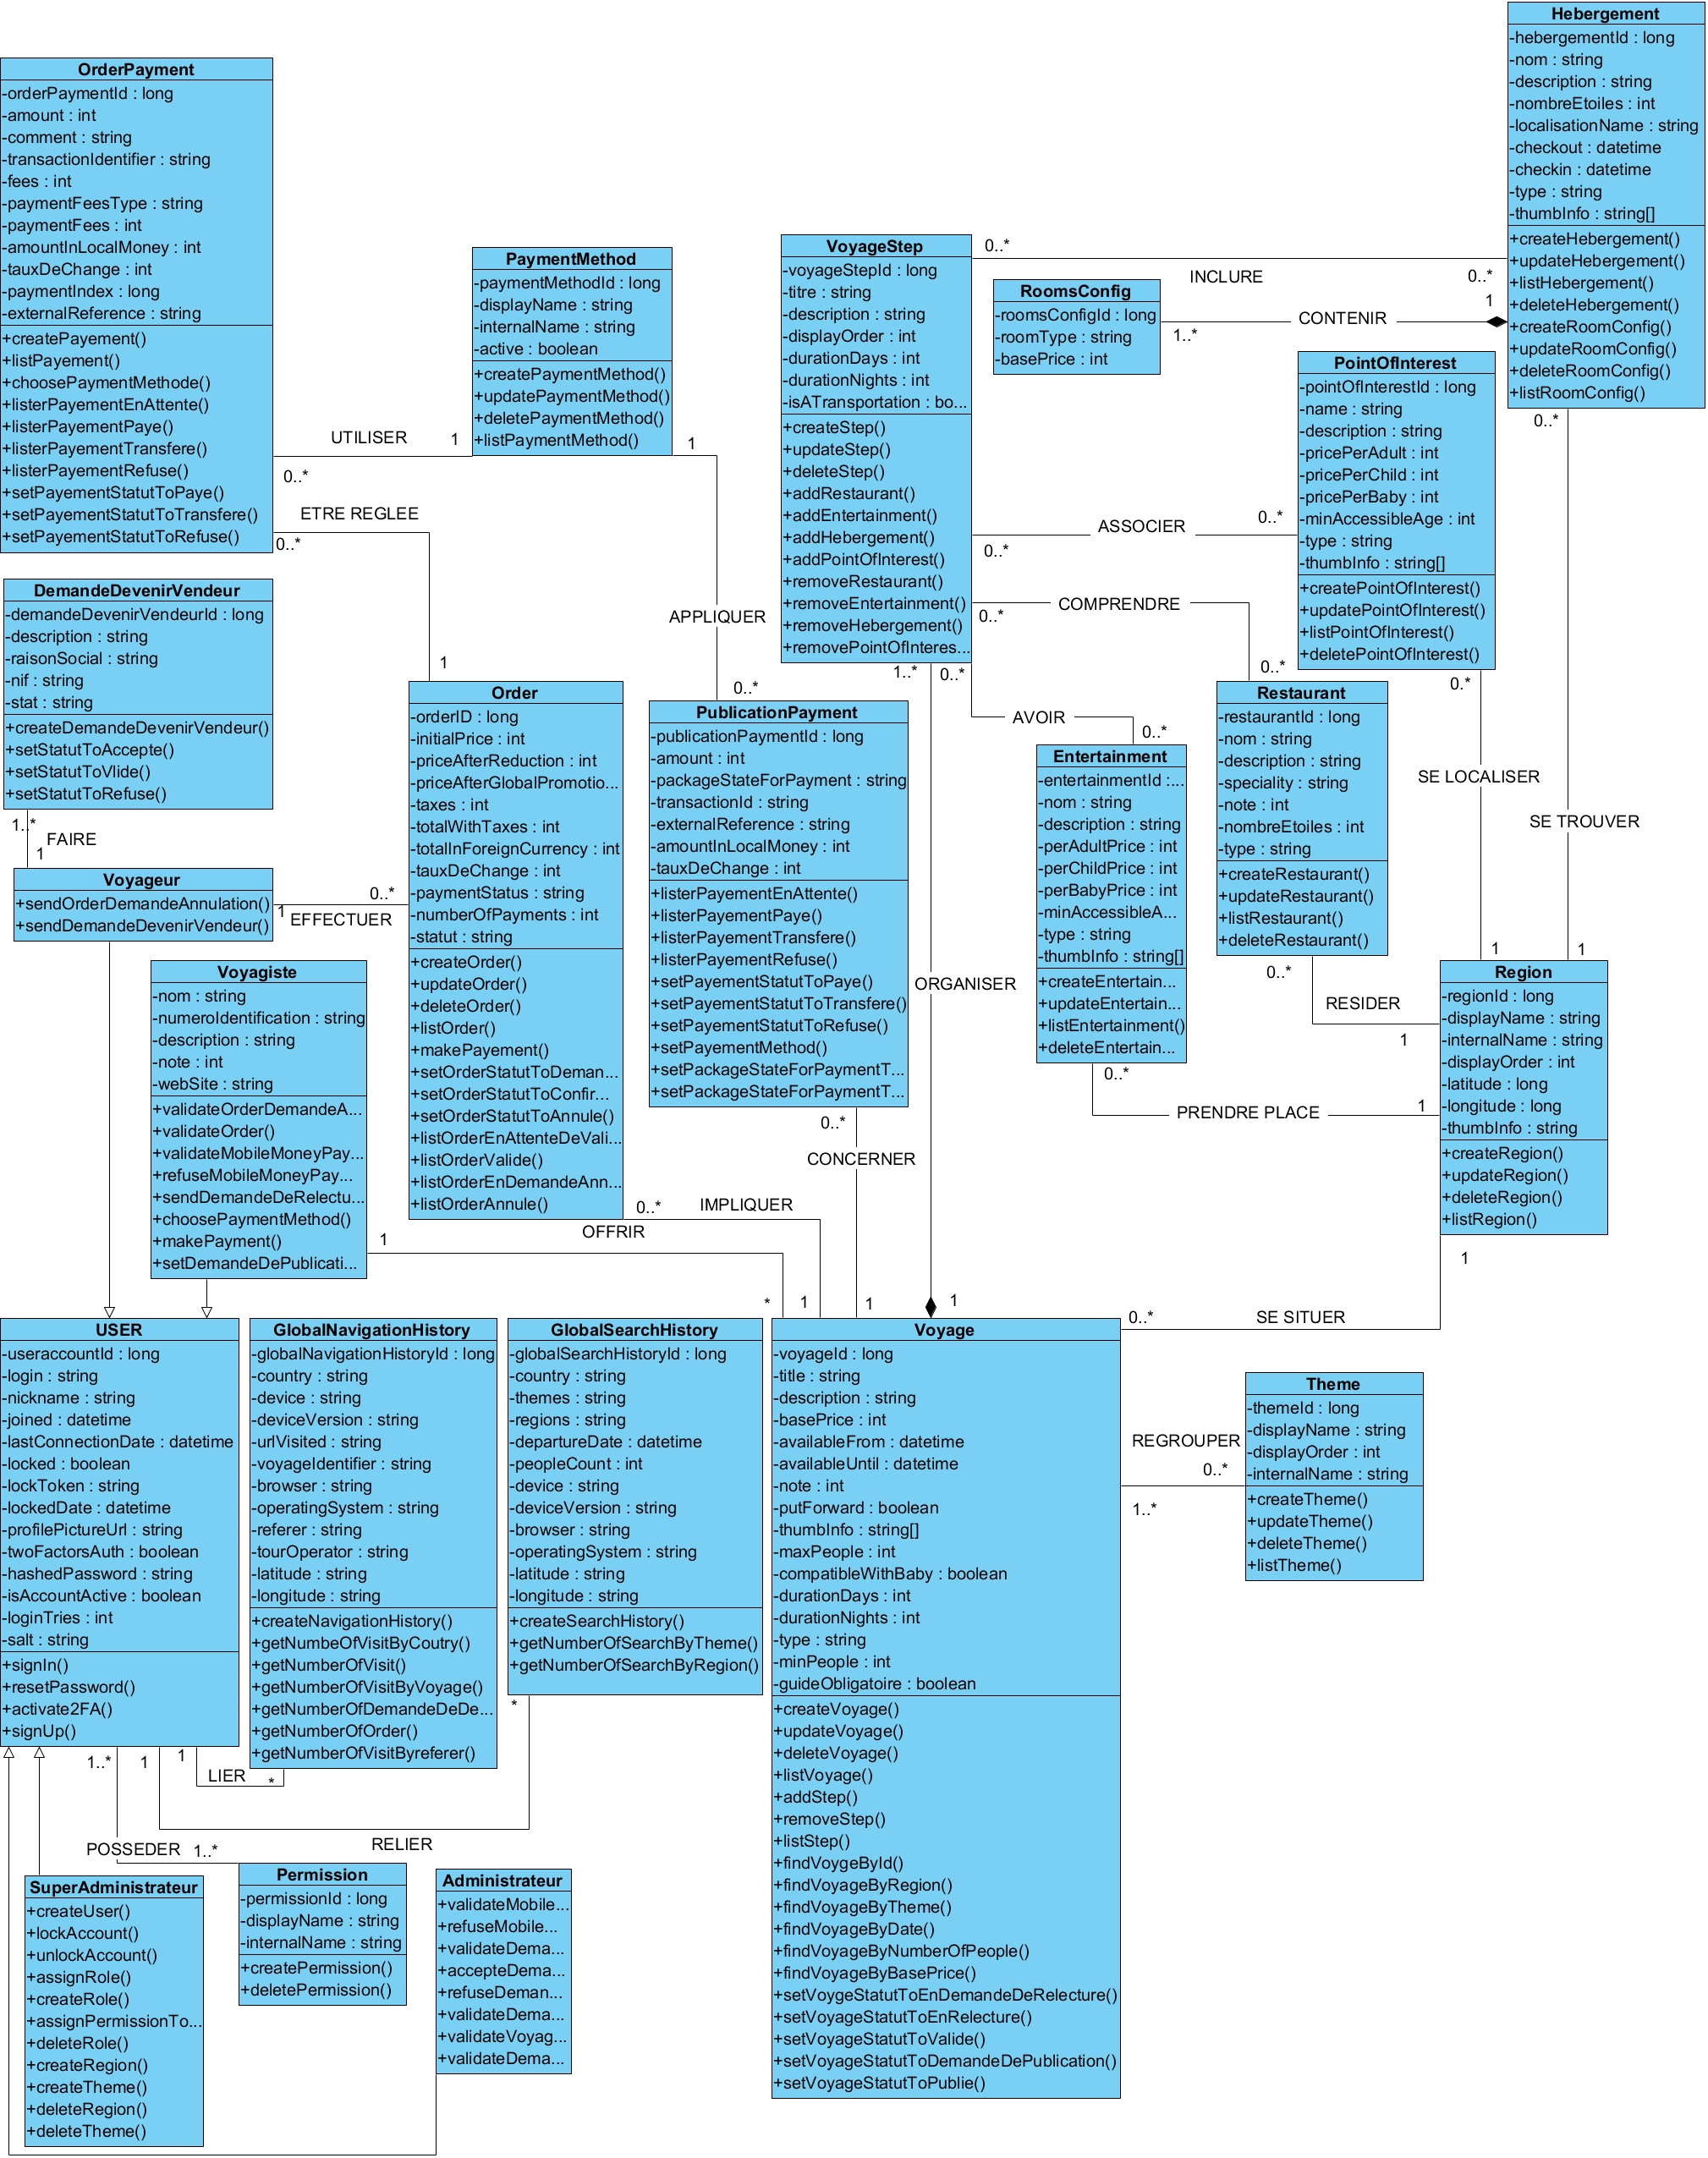
\includegraphics[width=\textwidth]{DCFinal.jpg}
				\caption{Diagramme de classe de conception globale du projet Handeha Voyage}
				\label{fig:DCFinal}
			\end{figure}
			\clearpage

	
			\section{Diagramme de paquetage}

			\hspace{15pt} Un Diagramme de paquetage est un type de diagramme UML qui montre l'organisation et la disposition des éléments de modèle dans un système en paquets, facilitant la gestion de la complexité en regroupant logiquement des éléments connexes et améliorant la lisibilité et la collaboration dans la conception et le développement.

			La figure \ref{fig:DPaquetage} représente le diagramme de paquetage du système.

			\begin{figure}[h]
				\centering
				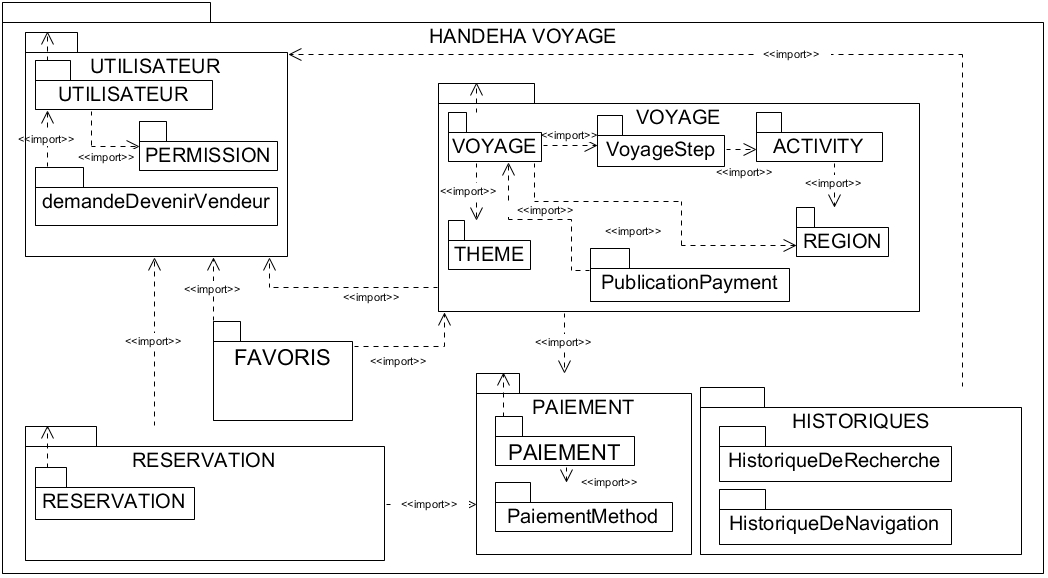
\includegraphics[width=\textwidth]{DPaquetage.jpg}
				\caption{Diagramme de paquetage du système du projet Handeha Voyage}
				\label{fig:DPaquetage}
			\end{figure}
			\clearpage


			\section{Diagramme de déploiement}
			
			\hspace{15pt} Un diagramme de déploiement est un type de diagramme UML qui montre la disposition physique des composants matériels et logiciels dans un système. Il est crucial pour visualiser la distribution des logiciels sur les nœuds matériels, comprendre l'architecture physique du système et identifier les éventuels goulets d'étranglement de performance.


			La figure \ref{fig:DDep} représente le diagramme de  de déploiement du système.

			\begin{figure}[h]
				\centering
				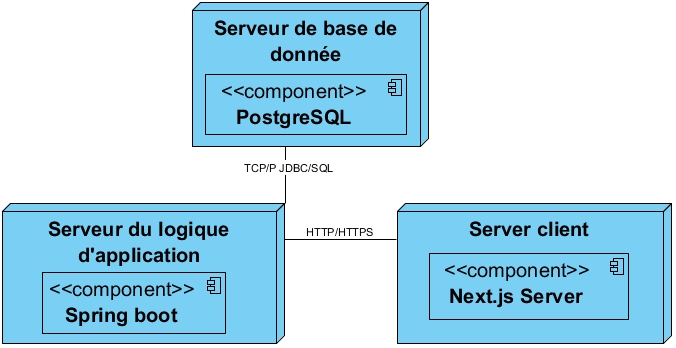
\includegraphics[width=\textwidth]{DDep.jpg}
				\caption{Diagramme  de déploiement du projet Handeha Voyage}
				\label{fig:DDep}
			\end{figure}
			\clearpage



			\part{REALISATION}

			\chapter{Mise en place de l’environnement de développement}

			\hspace{15pt} Ce chapitre vise à décrire les étapes nécessaires pour établir un environnement de développement efficace, facilitant ainsi la concrétisation de notre solution de conception. En informatique, la configuration d’un environnement de développement constitue une phase cruciale pour transformer une idée conceptuelle en une application fonctionnelle et intégrée sur divers supports.
			
			\section{Installation et configuration des outils}
			
			\hspace{15pt} Cette section détaille les étapes nécessaires pour installer et configurer les outils indispensables au développement de notre projet, assurant ainsi un environnement de travail efficace et bien préparé.

			\subsection{Installation de JDK}

			\hspace{15pt} Pour installer le JDK 21, nous commencerons par télécharger le kit de développement Java 21 depuis le site officiel d'Oracle. Nous choisirons la version correspondant à notre système d'exploitation Windows et suivrons les instructions de l'installateur pour finaliser l'installation.

			Une fois cette étape terminée, nous configurerons les variables d'environnement en ajoutant le chemin du JDK à notre système. Pour cela, nous définirons la variable JAVA HOME et mettrons à jour la variable PATH. Cela assurera que le système reconnaisse correctement le JDK.

			La figure \ref{fig:JDKVar} représente la configuration des variables d'environnement de JDK 21.

			\begin{figure}[h]
			    \centering
			    \begin{minipage}[t]{0.48\textwidth}
			        \centering
			        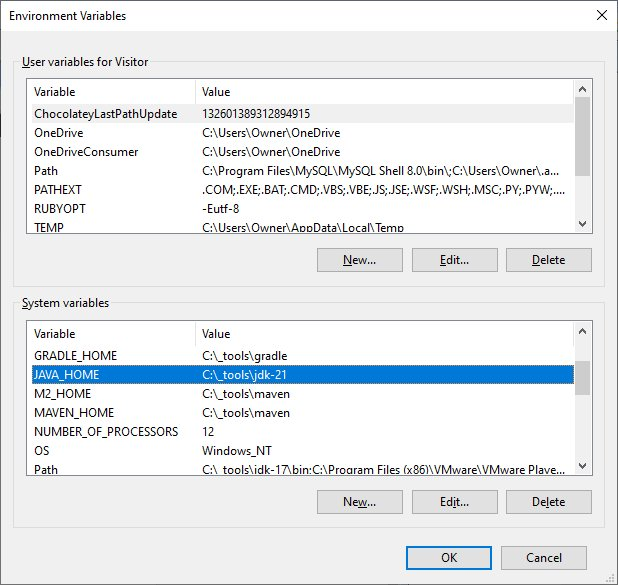
\includegraphics[width=\textwidth]{JAVAHOME.jpg}
			    \end{minipage}\hfill
			    \begin{minipage}[t]{0.48\textwidth}
			        \centering
			        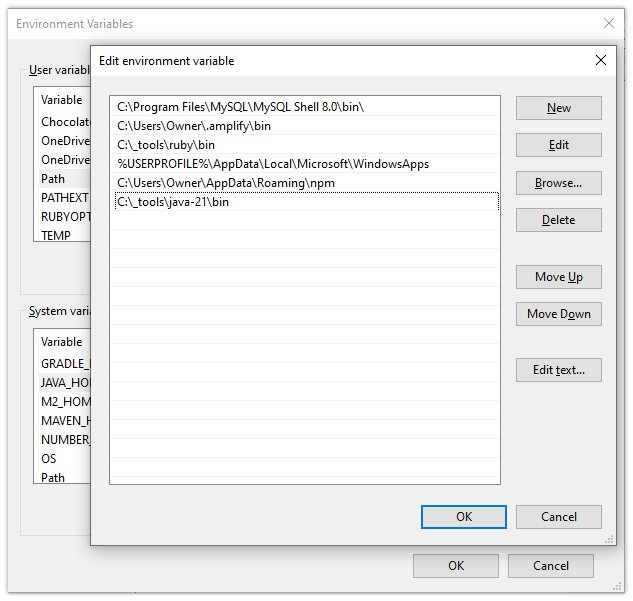
\includegraphics[width=\textwidth]{PATH.jpg}
			    \end{minipage}
			     \caption{Configuration des variables d'environnement de JDK 21}
			     \label{fig:JDKVar}
			\end{figure}
			\FloatBarrier
			
			Après avoir configuré les variables d'environnement, nous vérifierons l'installation en ouvrant une invite de commande ou un terminal et en tapant java -version. Cette commande nous permettra de confirmer que JDK 21 est installé et fonctionnel.

			\subsection{Installation de PostgreSQL}

			\hspace{15pt} Pour installer PostgreSQL, nous commencerons par télécharger la version correspondant à notre système d'exploitation depuis le site officiel de PostgreSQL. Après avoir lancé l'installateur et suivi les instructions à l'écran, nous configurerons un mot de passe pour l'utilisateur "postgres".

			La figure \ref{fig:postgreMDP} représente la  configuration du mot de passe pour l'utilisateur postgres.
			
			\begin{figure}[h]
				\centering
				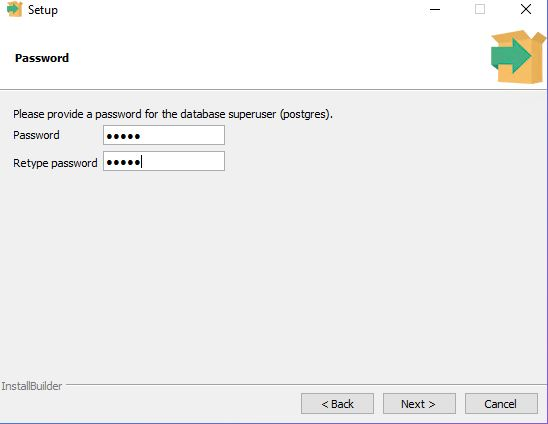
\includegraphics[width=0.6\textwidth]{postgreMDP.jpg}
				\caption{Configuration du mot de passe pour l'utilisateur postgres}
				\label{fig:postgreMDP}
			\end{figure}
			\FloatBarrier
	
			Une fois l'installation terminée, nous vérifierons que tout est correctement configuré en ouvrant une invite de commande ou un terminal et en tapant psql --version.

			\subsection{Installation des environnements de développements}
			
			\subsubsection{Visual Studio Code}

			\hspace{15pt} Pour installer Visual Studio Code, téléchargerons le à partir du site officiel de Microsoft. Une fois sur la page de téléchargement, nous choisirons la version correspondant à notre système d'exploitation.
			 Après avoir téléchargé le fichier d'installation, nous lancerons l'installateur et suivrons les instructions à l'écran pour finaliser l'installation.
			
			La figure \ref{fig:vscode} représente l’installation de Visual Studio Code.
			
			\begin{figure}[h]
				\centering
				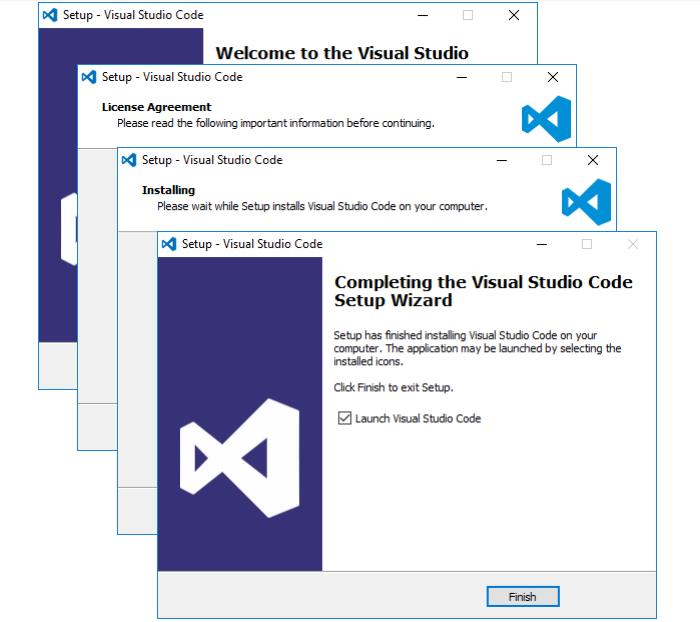
\includegraphics[width=0.6\textwidth]{vscode.png}
				\caption{Installation de Visual Studio Code}
				\label{fig:vscode}
			\end{figure}
			\FloatBarrier

			\subsubsection{Eclipse}

			\hspace{15pt} Pour installer Eclipse, nous commencerons par télécharger l'IDE Eclipse depuis le site officiel d'Eclipse. Une fois sur la page de téléchargement, nous sélectionnerons la version d'Eclipse IDE correspondant à notre système d'exploitation.

			Après avoir téléchargé le fichier d'installation, nous lancerons l'installateur et suivrons les instructions à l'écran pour finaliser l'installation.

			La figure \ref{fig:eclipseinstall} représente l’installation d'Eclipse.
			
			\begin{figure}[h]
				\centering
				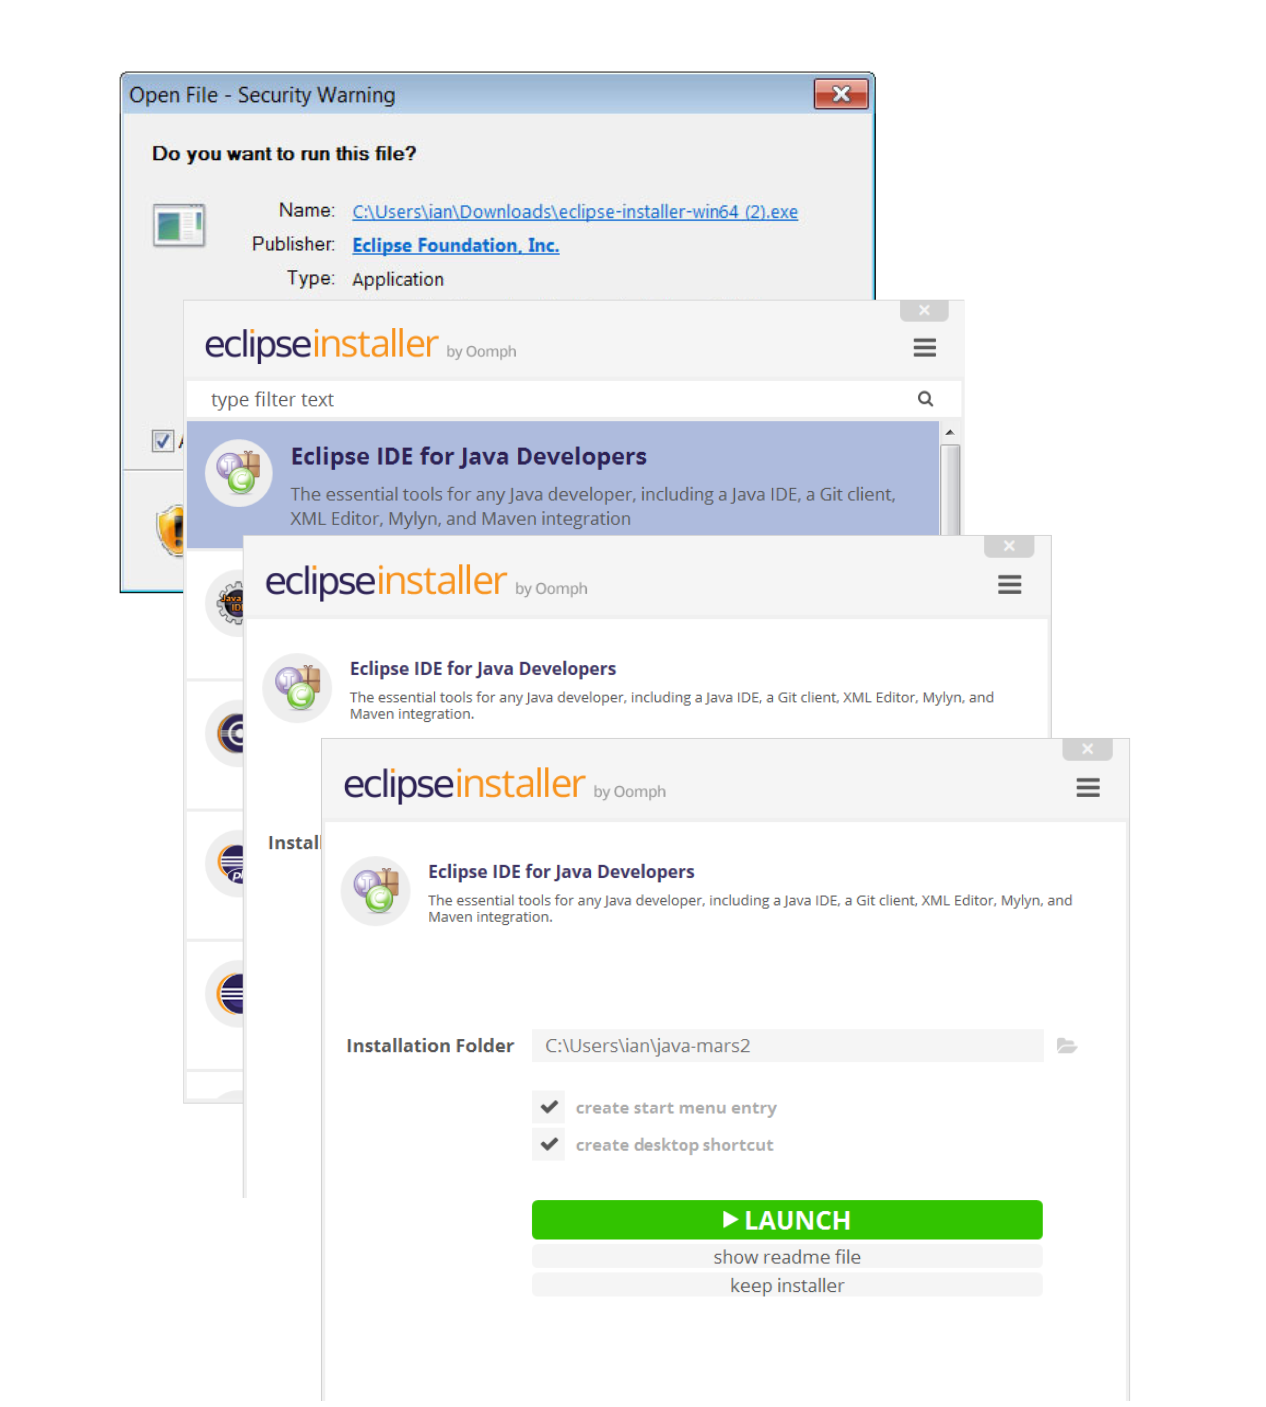
\includegraphics[width=0.6\textwidth]{eclipseinstall.png}
				\caption{Installation d'Eclipse}
				\label{fig:eclipseinstall}
			\end{figure}
			\FloatBarrier


			\subsubsection{Installation de Postman}

			\hspace{15pt} Pour installer Postman, nous commençons par télécharger l'application à partir du site officiel de Postman, en sélectionnant la version correspondant à notre système d'exploitation. Une fois le téléchargement terminé, nous ouvrons le fichier d'installation et suivons les instructions à l'écran. Après l'installation, nous lançons Postman et créons un compte ou nous connectons avec un compte existant.

			La figure \ref{fig:postman} représente l’installation de Postman.
			
			\begin{figure}[h]
				\centering
				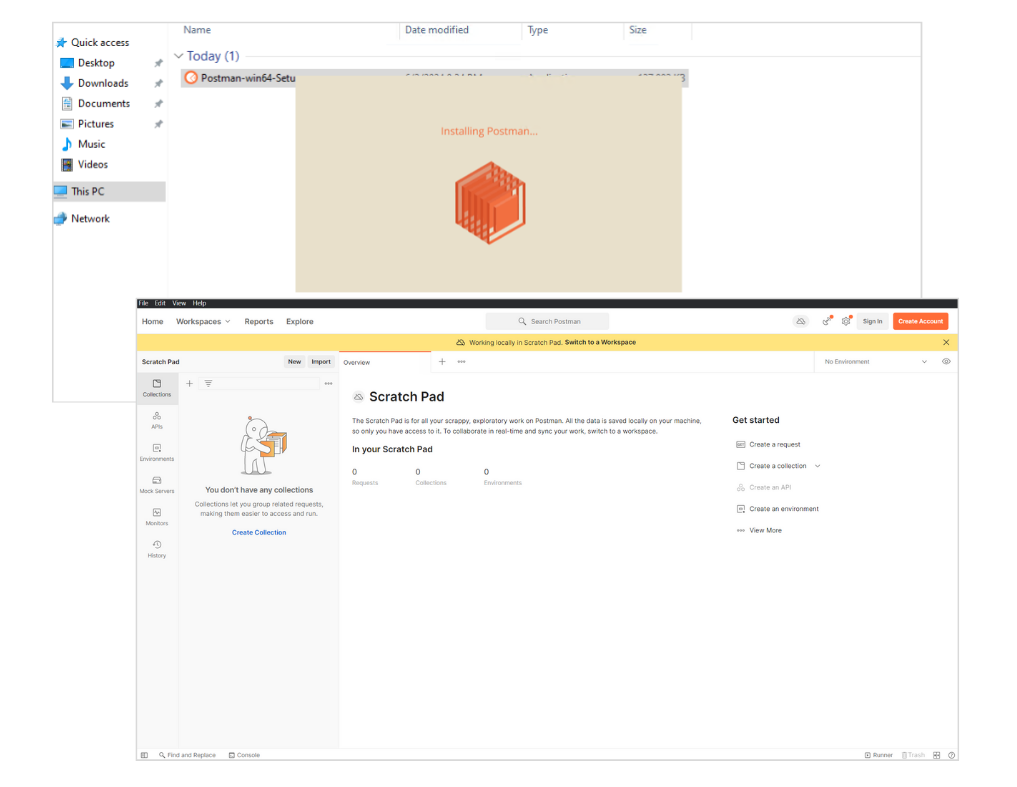
\includegraphics[width=0.6\textwidth]{postman.png}
				\caption{Installation de Postman}
				\label{fig:postman}
			\end{figure}
			\FloatBarrier
			
			\subsubsection{Installation de Visual Paradigm}

			\hspace{15pt} Pour installer Visual Paradigm, nous commençons par télécharger l'application depuis le site officiel de Visual Paradigm. Une fois le fichier d'installation téléchargé, nous l'exécutons et suivons les instructions à l'écran. Pendant l'installation, nous devrons accepter les termes de la licence.

			La figure \ref{fig:vispar} représente l’installation de Visual Paradigm.
			
			\begin{figure}[h]
				\centering
				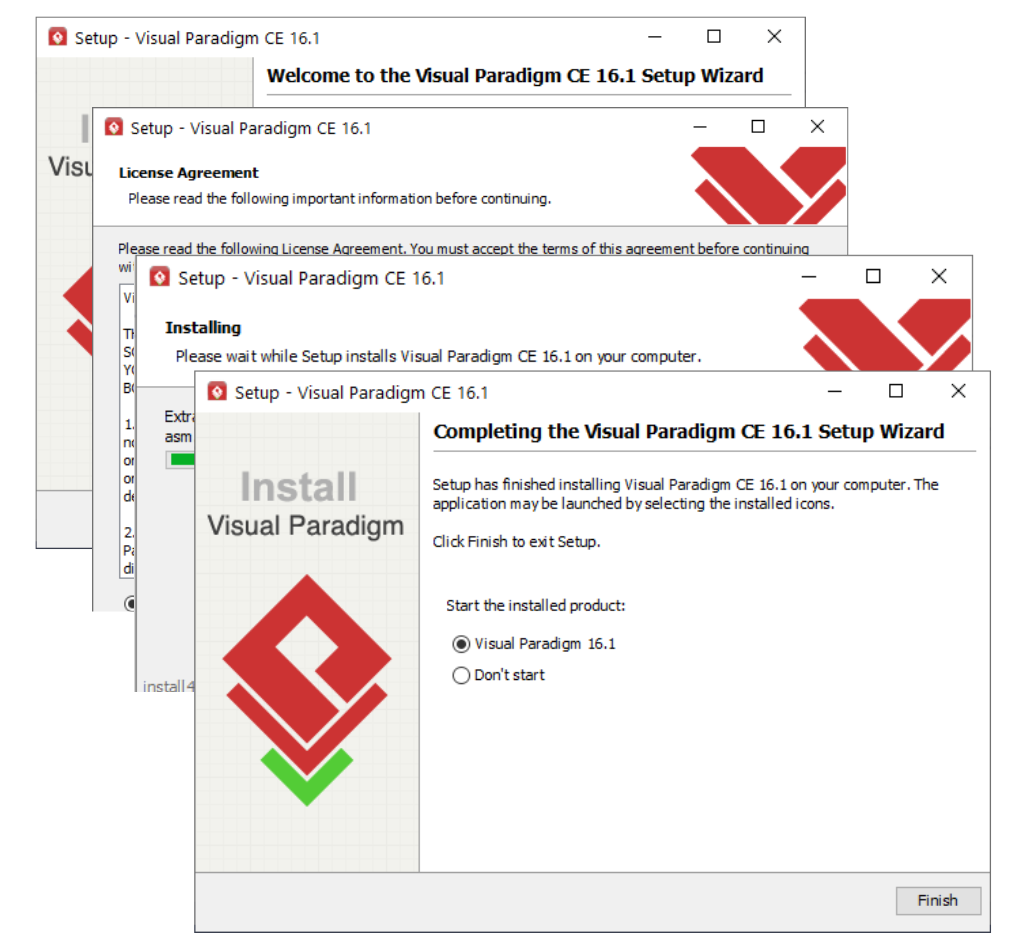
\includegraphics[width=0.6\textwidth]{vispar.png}
				\caption{Installation de Visual Paradigm}
				\label{fig:vispar}
			\end{figure}
			\FloatBarrier

			\subsubsection{Installation de Git}

			\hspace{15pt} Pour installer Git, nous commençons par télécharger l'application depuis le site officiel de Git. Une fois le fichier d'installation téléchargé, nous l'exécutons et suivons les instructions à l'écran. Pendant l'installation, nous acceptons les termes de la licence et choisissons les options par défaut, sauf indication contraire. Après avoir terminé l'installation, nous ouvrons un terminal ou une invite de commande et tapons git --version pour vérifier que Git est correctement installé. Si tout est en ordre, nous verrons la version de Git installée.

			La figure \ref{fig:git} représente l’installation de Git.
			
			\begin{figure}[h]
				\centering
				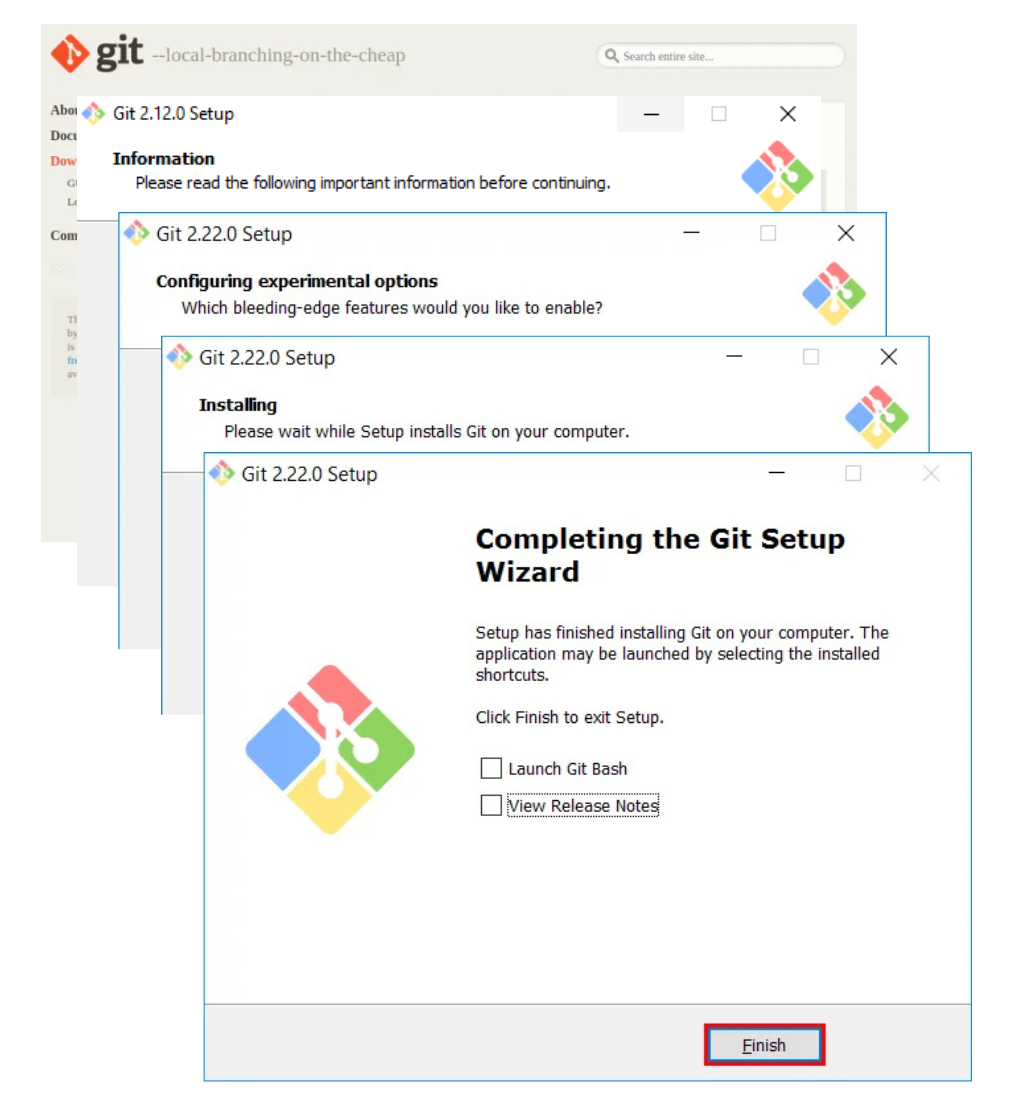
\includegraphics[width=0.6\textwidth]{git.png}
				\caption{Installation de Git}
				\label{fig:git}
			\end{figure}
			\FloatBarrier


			\section{Architecture de l’application}

			\hspace{15pt} Cette section décrit en détail l'architecture de notre application, en mettant en lumière les composants clés et leur interaction pour assurer une solution robuste, efficace et évolutive.

			\subsubsection{Architecture à trois tiers}
	
			\hspace{15pt} L'architecture de notre application est basée sur une approche à trois tiers, ce qui permet une séparation claire des responsabilités et facilite la gestion et la maintenance de l'application. Voici une description détaillée de chacun des tiers :

			Les trois tiers de l'architecture sont:

			\begin{itemize}
				\item \textbf{Tier Présentation ou Client:} Ce tier est responsable de l'interface utilisateur et de l'interaction avec les utilisateurs finaux. Il inclut les interfaces graphiques et les outils de navigation qui permettent aux utilisateurs d'interagir avec l'application. Ce tier peut être implémenté en utilisant des technologies web telles que HTML, CSS, JavaScript, ainsi que des frameworks modernes comme React, Angular ou Vue.js.Pour les applications mobiles, des outils comme Flutter ou React Native peuvent être utilisés.
				\item \textbf{Tier Logique d'Application ou Serveur d'application:} Ce tier contient la logique métier de l'application, c'est-à-dire les règles et les traitements nécessaires pour répondre aux besoins fonctionnels de l'application. Il assure le traitement des données reçues du client et l'application des règles métiers avant d'interagir avec la base de données. Les serveurs d'application peuvent être construits avec divers langages de programmation et frameworks tels que Java avec Spring Boot, Node.jsavec Express, ou encore Python avec Django ou Flask.	
				\item \textbf{Tier Base de Données ou Serveur de BD:} Ce tier est responsable de la gestion, du stockage et de la récupération des données nécessaires au bon fonctionnement de l'application. Il communique avec le tier de logique d'application pour fournir les données requises et stocker les nouvelles informations.Les bases de données relationnelles comme PostgreSQL, MySQL ou Oracle peuvent être utilisées. Pour des besoins spécifiques, des bases de données NoSQL comme MongoDB peuvent également être envisagées.
			\end{itemize}

			La figure \ref{fig:archi3T} représente l’architecture à trois tiers.
			
			\begin{figure}[h]
				\centering
				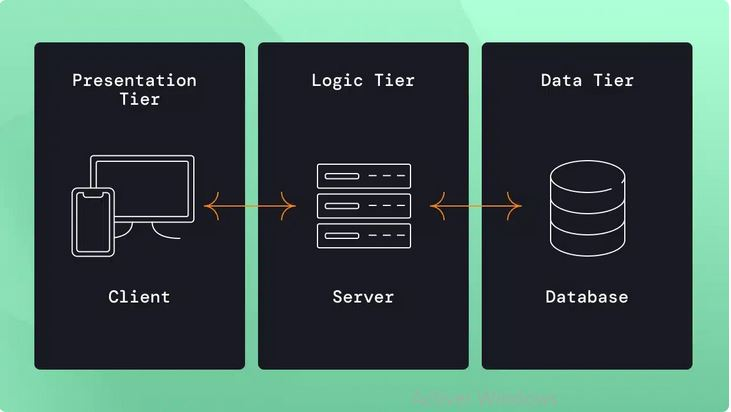
\includegraphics[width=\textwidth]{archi3T.jpg}
				\caption{Architecture à trois tiers\cite{3Tier}}
				\label{fig:archi3T}
			\end{figure}
			\FloatBarrier


			\chapter{Développement de l’application}


			\hspace{15pt} Le développement de l'application est une étape cruciale dans notre projet, où les idées et concepts prennent vie pour devenir un produit fonctionnel adapté aux besoins des utilisateurs. Dans cette section, nous décrirons les étapes essentielles du processus de développement, telles que la mise en place de la base de données, l'implémentation des différentes fonctionnalités, ainsi que la présentation du résultat final.
		
			\section{Création de la base de données}
			
			\hspace{15pt} Cette section détaille le processus de création de la base de données, une étape cruciale pour assurer une gestion efficace et structurée des informations nécessaires au bon fonctionnement de l'application.

			Pour créer la base de données, nous utiliserons PgAdmin. Les étapes précises sont les suivantes :					

			\begin{itemize}
				\item \textbf{Lancement de PgAdmin:} Ouvrir PgAdmin et se connecter au serveur PostgreSQL
				\item \textbf{Navigation vers les Bases de Données:} Dans le volet de navigation à gauche, faire un clic droit sur "Databases" sous le serveur, puis sélectionner "Create" et ensuite "Database...".
				\item \text{Création de la Base de Données:} Une fenêtre de configuration s'ouvre. Dans le champ "Database", entrer le nom de la base de données, ici "handeha" puis cliquer sur "Save" pour finaliser la création.
			\end{itemize}

			La figure \ref{fig:DbCreation} représente la création de base de donnée du projet Handeha Voyage.
			
			\begin{figure}[h]
				\centering
				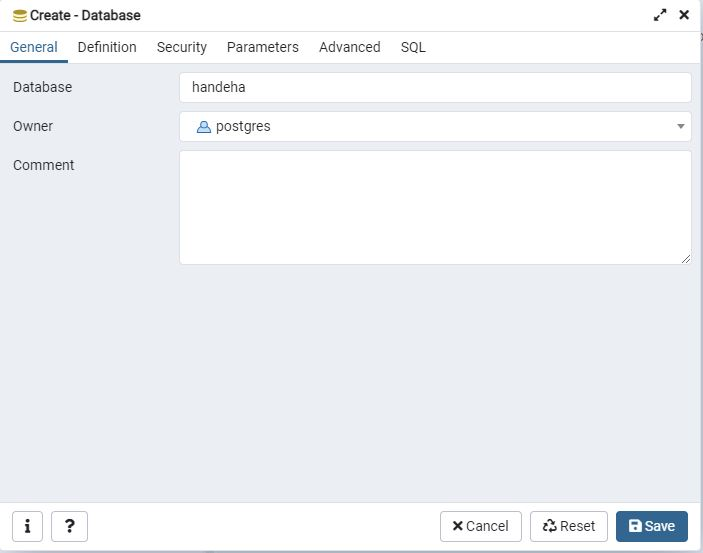
\includegraphics[width=0.8\textwidth]{DbCreation.jpg}
				\caption{Création de base de donnée du projet Handeha Voyage}
				\label{fig:DbCreation}
			\end{figure}
			\FloatBarrier


			Maintenant que notre base de données est créée, il est temps de permettre à notre projet de communiquer avec une base de données PostgreSQL en ajoutant la dépendance PostgreSQL dans le fichier "pom.xml" de notre projet.

			La figure \ref{fig:pomPostgre} représente l'ajout de la dépendance PostgreSQL dans le fichier "pom.xml".
			
			\begin{figure}[h]
				\centering
				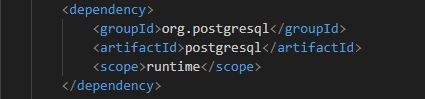
\includegraphics[width=0.8\textwidth]{pomPostgre.jpg}
				\caption{Ajout de la dépendance PostgreSQL dans le fichier "pom.xml".}
				\label{fig:pomPostgre}
			\end{figure}
			\FloatBarrier

			Nous devons également configurer notre application Spring Boot pour qu'elle puisse interagir avec une base de données PostgreSQL. Cette configuration se réalise dans le fichier "application.properties".
	

			La figure \ref{fig:appPropPostgre} représente la configuration de Spring Boot pour une base de données PostgreSQL.
			
			\begin{figure}[h]
				\centering
				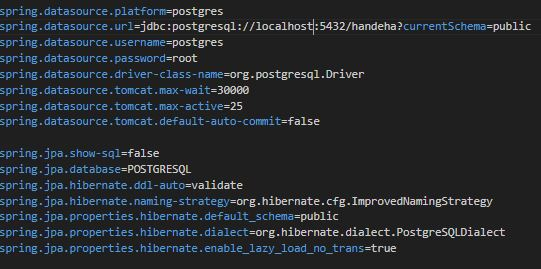
\includegraphics[width=\textwidth]{appPropPostgre.jpg}
				\caption{Configuration de Spring Boot pour une base de données PostgreSQL}
				\label{fig:appPropPostgre}
			\end{figure}
			\FloatBarrier

			Grâce aux annotations fournies par l'ORM Hibernate, il suffit de démarrer le serveur backend en exécutant la commande mvn clean install -PdropDb,updateDb. Cette commande exécutera le script de création de tables pour notre base de données.


			\section{Codage de l’application}

			\hspace{15pt} Cette section aborde le codage de l'application, décrivant les méthodologies, les outils et les pratiques de développement que nous avons adoptés pour transformer nos concepts en une solution fonctionnelle et performante.

			\subsection{Côté Back-end}
			
			\hspace{15pt} Le back-end de notre application gère la logique métier, les interactions avec la base de données et la communication avec le front-end. Il est essentiel pour le traitement des données et la mise en œuvre des fonctionnalités principales.

			Notre projet back-end est structuré en plusieurs packages pour une meilleure organisation :

			\begin{itemize}
				\item \textbf{controller:} Contient les contrôleurs REST qui gèrent les requêtes des utilisateurs;
				\item \textbf{service:} Contient la logique métier, c'est-à-dire les règles et les calculs;
				\item \textbf{repository:} Contient les interfaces pour accéder aux données dans la base de données;
				\item \textbf{model:} Contient les entités, qui représentent les tables dans la base de données.
			\end{itemize}

			\subsubsection{Entités JPA et Mappage}

			\hspace{15pt} Les entités JPA sont comme des plans pour les tables de la base de données. Elles sont définies comme suit:

			La figure \ref{fig:entityjpa} représente la définition d'une entité pour les voyages.
			
			\begin{figure}[h]
				\centering
				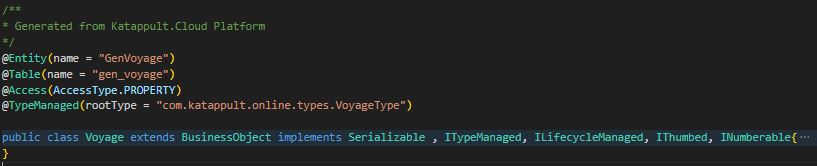
\includegraphics[width=\textwidth]{entityjpa.jpg}
				\caption{Entité pour les voyages}
				\label{fig:entityjpa}
			\end{figure}
			\FloatBarrier

			\begin{itemize}
				\item @Entity : Indique que cette classe représente une table dans la base de données.
				\item @Table(name = "gen voyage") : Spécifie le nom de la table dans la base de données.
				\item @Access(AccessType.PROPERTY) : Indique que JPA doit utiliser les méthodes getter et setter pour accéder aux attributs de l'entité, au lieu d'accéder directement aux champs.
			\end{itemize}
	
			Les entités JPA sont composées de propriétés qui représentent les colonnes de la table de la base de données, et de méthodes pour accéder et manipuler ces propriétés.

			La figure \ref{fig:propmeth} représente une extrait des propriétés et methodes de l' entité pour les voyages.
			
			\begin{figure}[h]
				\centering
				\includegraphics[width=\textwidth]{propmeth.jpg}
				\caption{Extrait des propriétés et methodes de l' entité pour les voyages}
				\label{fig:propmeth}
			\end{figure}
			\FloatBarrier

			\begin{itemize}
				\item titre et description sont des propriétés, getOid, getTitle, setTitle, getDescription, setDescription sont des méthodes.
				\item @Id : Signifie que cet attribut est la clé primaire.
				\item @GeneratedValue : Indique que la valeur de l'identifiant est générée par la séquence définie.
				\item @SequenceGenerator : Définit un générateur de séquence nommé "gen-voyage-oid-seq" qui utilise la séquence "gen-voyage-oid-seq" pour générer des valeurs. allocationSize=1 spécifie la taille de l'allocation de la séquence.
				\item @Column(columnDefinition = "serial", updatable = false) : Spécifie que cette colonne est de type "serial" et ne peut pas être mise à jour.
				\item @Column(name = "title") : Spécifie que cette propriété est mappée à la colonne "title" de la table de base de données.
			\end{itemize}
			
			
			\subsubsection{Services et Logique Métier}

			\hspace{15pt} Les services sont les cerveaux de l'application.Les services sont définies comme suit:

			La figure \ref{fig:service} représente la définition du service pour les résvation des voyages.
			
			\begin{figure}[h]
				\centering
				\includegraphics[width=\textwidth]{service.jpg}
				\caption{Définition du service pour les résvation des voyages}
				\label{fig:service}
			\end{figure}
			\FloatBarrier

			\begin{itemize}
				\item @Service : Indique que cette classe est un service, un composant métier dans Spring.
			\end{itemize}

			Les services sont composés d'Injection de Dépendances et Logique Métier.

			La figure \ref{fig:methService} représente une extrait des Injection de Dépendances et Logique Métier du service pour les résvation des voyages.
			
			\begin{figure}[h]
				\centering
				\includegraphics[width=\textwidth]{methService.jpg}
				\caption{Extrait des Injection de Dépendances et Logique Métier du service pour les résvation des voyages}
				\label{fig:methService}
			\end{figure}
			\FloatBarrier

			\begin{itemize}
				\item Les propriétés comme repository ici représentent les dépendances. Les méthodes comme create, addOrderPayment sont les logiques métier.
				\item @Autowired : Utilisée pour injecter automatiquement les dépendances nécessaires, comme les repositories, dans le service. Ici nous utilisant le constructeur OrderServiceImpl pour injecter les dépendances.
				\item @Transactional : Utilisée pour gérer les transactions, garantissant que les opérations sur la base de données sont exécutées de manière atomique et cohérente.
			\end{itemize}
			

			\subsubsection{Contrôleurs REST}
			
			\hspace{15pt} Les contrôleurs REST gèrent les requêtes des utilisateurs. Les contrôleurs sont définies comme suit:

			La figure \ref{fig:controleur} représente la définition du contrôleur pour les résvation des voyages.
			
			\begin{figure}[h]
				\centering
				\includegraphics[width=\textwidth]{controleur.jpg}
				\caption{Définition du contrôleur pour les résvation des voyages}
				\label{fig:controleur}
			\end{figure}
			\FloatBarrier

			\begin{itemize}
				\item @RestController Indique que cette classe est un contrôleur où chaque méthode retourne une entité de domaine plutôt qu'une vue.
				\item @RequestMapping Spécifie l'URL de base pour toutes les requêtes traitées par ce contrôleur.
			\end{itemize}

			Les contrôleurs ont souvent des services comme dépendances et des méthodes HTTP pour répondre aux requêtes utilisateurs.

			La figure \ref{fig:contenuscontroleur} représente l'extrait des contenus du contrôleur pour les résvation des voyages.
			
			\begin{figure}[h]
				\centering
				\includegraphics[width=\textwidth]{contenuscontroleur.jpg}
				\caption{Extrait contenus du contrôleur pour les résvation des voyages}
				\label{fig:contenuscontroleur}
			\end{figure}
			\FloatBarrier
			\begin{itemize}
				\item Dans un contrôleur les propriétés représentent des dépendances et les méthodes des méthodes HTTP.
				\item @GetMapping : Pour les requêtes de récupération de données.
				\item @PostMapping : Pour les requêtes de création de nouvelles données.
				\item @PutMapping : Pour les requêtes de mise à jour de données existantes.
				\item @DeleteMapping : Pour les requêtes de suppression de données.
			\end{itemize}
			

			\subsection{Côté Front-end}

			\hspace{15pt} Le front-end de notre application gère l'interface utilisateur et l'expérience utilisateur. Il est essentiel pour présenter les données de manière conviviale et interactive. Notre projet front-end est structuré en plusieurs parties pour une meilleure organisation :

			\begin{itemize}
				\item \textbf{Composants:} Les composants sont les blocs de construction de l'interface utilisateur. Ils sont réutilisables et encapsulent leur propre logique et style.
				\item  \textbf{Pages:} Les pages sont des composants spéciaux qui représentent des routes spécifiques dans l'application.
				\item \textbf{Services API:} Les services API sont utilisés pour interagir avec le backend, récupérer et envoyer des données.
			\end{itemize}

			\subsubsection{Composants}
			\hspace{15pt} Un composant est une petite partie de l' interface utilisateur qui est indépendante et réutilisable. Chaque composant gère sa propre apparence et son propre comportement, ce qui facilite la construction et la maintenance des applications web.

			La figure \ref{fig:component} représente l'extrait d'un composant.
			
			\begin{figure}[h]
				\centering
				\includegraphics[width=\textwidth]{component.jpg}
				\caption{Extrait d'un composant}
				\label{fig:component}
			\end{figure}
			\FloatBarrier
			
			Le composant ValidationCommandeStep2WithoutStripe est ici composé de:

			\begin{itemize}
				\item \textbf{Propriétés ou props:} Ici quotation, previousStep, contactAndBillingForm, nextStep et voyage. Ce sont des données passées d'un composant parent à un composant enfant, permettant de personnaliser le comportement et l'affichage du composant.
				\item \textbf{État ou State:} Ici processingOrder , errors et agreementChecked. Ce sont les données spécifiques à un composant qui peuvent changer au fil du temps. L'état est utilisé pour rendre l'interface utilisateur réactive aux interactions.
				\item \textbf{Méthodes:} Ici validatePayment et goPrevious. Ce sont les fonctions définies dans le composant pour gérer les interactions utilisateur, les calculs ou toute autre logique nécessaire.
				\item \textbf{Rendu ou Render:} La partie du composant qui renvoie le JSX, définissant ce qui sera affiché à l'utilisateur.
			\end{itemize}

			\subsubsection{Pages}
			\hspace{15pt} En Next.js, une page est essentiellement un composant React qui est utilisé pour définir une route dans l'application. Chaque fichier dans le répertoire pages d'un projet Next.jscorrespond à une route unique à laquelle les utilisateurs peuvent naviguer.
			
			La figure \ref{fig:pages} représente l'extrait d'une Pages.
			
			\begin{figure}[h]
				\centering
				\includegraphics[width=\textwidth]{pages.jpg}
				\caption{Extrait d'une Pages}
				\label{fig:pages}
			\end{figure}
			\FloatBarrier

			\begin{itemize}
				\item La page BookingPage est accessible à travers une route définie par sa position dans le répertoire pages;
				\item Son contenu est généré par le composant BookingContainer;
				\item Grâce à getLayout, cette page est rendue avec la même mise en page que la page d'accueil.
 			\end{itemize}

			\subsubsection{Services API}

			\hspace{15pt} Une services API dans une application Next.js est un ensemble de fonctions qui facilitent la communication entre le frontend et le backend. Ces fonctions sont essentielles pour effectuer des opérations CRUD et gérer le flux de données entre les deux parties de l'application.

			La figure \ref{fig:serviceAPI} représente l'extrait d'une services API.
			
			\begin{figure}[h]
				\centering
				\includegraphics[width=0.8\textwidth]{serviceAPI.jpg}
				\caption{Extrait d'une services API}
				\label{fig:serviceAPI}
			\end{figure}
			\FloatBarrier

			\begin{itemize}
				\item Ici nous avons une services API nomée OrderService qui expose un fonction nomée payABooking;
				\item Cette fonction permet d'effectuer un paiement pour une réservation en envoyant une requête POST à un serveur. Elle utilise un identifiant de réservation et un formulaire pour transmettre les données nécessaires;
				\item Cette fonction gère les requêtes POST de en utilisant Axios;
				\item Le mot-clé await permet d'attendre la réponse de manière asynchrone;	
				\item Configuration d’Axios : Temps limite de 15 secondes, type de contenu "application/json", acceptation "application/json".
			\end{itemize}
			


			\section{Présentation de l’application}












		


			\chapter*{CONCLUSION}
			\addcontentsline{toc}{chapter}{CONCLUSION}	

			\hspace{15pt} Ce mémoire a mis en lumière les défis et les opportunités liés à la promotion du secteur touristique à Madagascar à travers la digitalisation des services. Face à une demande croissante pour des expériences de voyage personnalisées et une visibilité accrue des opérateurs locaux, l'application Handeha Voyage propose une solution innovante et pratique.\\

			Le processus de conception, de développement et de mise en œuvre de l’application a permis de répondre aux objectifs initiaux, à savoir faciliter la mise en ligne des offres touristiques, simplifier la réservation pour les voyageurs et offrir une meilleure visibilité aux opérateurs malgaches. Grâce à des outils modernes tels que UML pour la modélisation, Next.js pour le front-end, Spring Boot pour le back-end, et PostgreSQL comme Système de Gestion de Base de Données, ainsi qu’une méthodologie de gestion de projet rigoureuse basée sur Agile-Scrum et accompagnée de l’outil Trello, nous avons pu poser les bases d’une plateforme qui redéfinit la manière dont les services touristiques sont consommés.\\

			Cependant, certaines limitations, comme le temps restreint pour le développement de fonctionnalités avancées et l’accès limité aux retours d’expérience en cours de projet, ont laissé des pistes d’amélioration. Ces défis n’entachent en rien la pertinence et le potentiel de l’application, mais ouvrent plutôt des perspectives intéressantes pour son évolution future.\\

			À l’avenir, il serait essentiel d’intégrer des fonctionnalités supplémentaires, comme l’analyse des comportements des utilisateurs ou l’optimisation des interactions avec les opérateurs, afin d’enrichir l’expérience utilisateur. Par ailleurs, un partenariat étroit avec les acteurs du tourisme local pourrait maximiser l’impact de cette solution et contribuer à dynamiser davantage ce secteur clé de l’économie malgache.\\

			Ainsi, Handeha Voyage ne représente pas seulement une plateforme technologique, mais aussi un outil stratégique pour la valorisation de la richesse touristique de Madagascar. Nous espérons que cette initiative contribuera significativement au développement du tourisme local tout en offrant des opportunités aux opérateurs et des expériences mémorables aux voyageurs.
			
			
			\newpage
			\pagenumbering{roman}
			\renewcommand{\thepage}{\Roman{page}} % Ensure uppercase Roman numerals
			\setcounter{page}{10}
 
			\begin{thebookbibliography}{9}
				\bibitem[1]{ScrumGuide} Ken Schwaber and Jeff Sutherland, \textit{« The Scrum Guide »}, 2020.
				\bibitem[2]{Bennett} Simon Bennett, \textit{« Schaum's Outline of UML »}, McGraw-Hill, 2nd
				\bibitem[3]{PostgreSQLExperience} Pavel Luzanov, Egor Rogov, and Igor Levshin, \textit{« PostgreSQL: The First Experience »}, 2023.
				\bibitem[4]{Eckel} Bruce Eckel, \textit{« Thinking in Java »}, Prentice Hall, 4th edition, 2006.
				\bibitem[5]{Tsitoara} Mariot Tsitoara, \textit{« Beginning Git and GitHub: A Comprehensive Guide to Version Control, Project Management, and Teamwork for the New Developer »}, Apress, 2019.
			\end{thebookbibliography}
	

			\begin{thewebography}{9}
				\bibitem [6]{Doc4Dev} \url{https://doc4dev.com/comparaison-des-differentes-methodes-de-gestion-de-projet-avantages-inconvenients-et-exemples}, \textit{« Comparaison des différentes méthodes de gestion de projet : avantages, inconvénients et exemples »} , consulté le : 15 septembre 2024.
				\bibitem[7]{Asana} \url{https://asana.com/fr/resources/agile-methodology}, \textit{« Qu'est-ce que la méthode Agile? »} , consulté le : 19 septembre 2024.
				\bibitem[8]{pm-partners} \url{https://www.pm-partners.com.au/insights/the-agile-journey-a-scrum-overview/}, \textit{« What is Scrum? An overview of Scrum and The Agile Journey »}, consulté le : 24 septembre 2024.
 				\bibitem[9]{VisualParadigm} \url{https://www.visual-paradigm.com/support/documents/vpuserguide/100/2450/78667_seetheevolut.html}, \textit{« Visual Paradigm User's Guide »} , consulté le : 2 octobre 2024. 
				\bibitem[10]{SpringFramework}  \url{https://spring.io/spring-framework}, \textit{« Spring Framework »} , consulté le : 10 octobre 2024.
				\bibitem[11]{JavaScriptHistory} \url{https://www.w3schools.com/js/js_history.asp}, \textit{« JavaScript History »}, consulté le : 18 octobre 2024.
				\bibitem[12]{NextJS}  \url{https://nextjs.org/docs} \textit{« Next.js Documentation »}, 28 octobre 2024.	
				\bibitem[13]{katappult} \url{https://www.katappult.cloud/}, \textit{« Katappult - Plateforme Low-Code pour la Création d’Applications Web et Mobiles »} , consulté le : 11 juillet 2024.
				\bibitem[14]{3Tier} \url{https://vfunction.com/blog/3-tier-application/}, \textit{« What is a 3-tier application architecture? Definition and Examples »}, consulté le : 10 novembre 2024.
			\end{thewebography}


			\chapter*{GLOSSAIRE}
			\addcontentsline{toc}{chapter}{GLOSSAIRE}	
			
			\textbf{2FA:} L’authentification à deux facteurs est une méthode de sécurité qui nécessite deux formes de vérification pour accéder à un compte.\\
			\textbf{Voyage:} Un voyage se réfère à un déplacement planifié et organisé principalement pour des raisons touristiques ou des vacances.\\
			\textbf{Circuit:} Un circuit se réfère à un voyage pré-planifié et organisé qui emmène les voyageurs à travers une série de destinations, d'activités et d'expériences.\\
			\textbf{Séjour:} Un séjour se réfère à une période de temps passée à un endroit spécifique pour des raisons de loisirs, de détente ou de vacances.\\
			\textbf{Thème:} Concept ou une idée centrale qui guide la planification et l'organisation du voyage.\\
			\textbf{Transaction:} une transaction fait référence à l'ensemble du processus d'achat ou de réservation d'un voyage.\\
			\textbf{Méthode de paiement:} Une méthode de paiement sur une plateforme de réservation touristique est un moyen par lequel les utilisateurs peuvent régler leurs réservations.\\
			\textbf{Prix de base:} Le prix de base fait référence au coût initial ou standard par personne d'un voyage ou activité ou service avant l'ajout de frais supplémentaires ou de taxes.\\
			\textbf{Service:} Les services se réfèrent aux diverses prestations et commodités offertes pour améliorer l'expérience du voyageur.\\
			\textbf{Activité:} Une activité se réfère aux diverses expériences et loisirs que les voyageurs peuvent planifier et réaliser pendant leur séjour ou circuit. Les activités sont souvent des éléments clés pour enrichir l'expérience de voyage.\\
			\textbf{Guide:} Un professionnel qui accompagne les voyageurs pour fournir des informations, des explications et des anecdotes sur les lieux visités.\\
			\textbf{Remise:} Les remises se réfèrent aux réductions ou offres spéciales qui permettent aux voyageurs de bénéficier de prix réduits sur leurs réservations.\\
			\textbf{Point d'intérêt:} Un point d'intérêt dans le contexte d'un voyage se réfère à un lieu ou une attraction qui mérite d'être visité en raison de son importance culturelle, historique, naturelle, ou de loisirs.\\
			\textbf{Pension:} La pension fait référence aux repas inclus pendant le voyage.\\
			\textbf{Taxes:} Les taxes peuvent inclure plusieurs types de frais supplémentaires imposés par les gouvernements et autres autorités.\\
			\textbf{Devise:} Une devise se réfère à la monnaie utilisée dans un pays spécifique.\\
			\textbf{tauxDeChange:} Les taux de change sont les valeurs par lesquelles une devise est échangée contre une autre.\\
			\textbf{voyagiste:} Un voyagiste est une entreprise spécialisée dans l'organisation de voyages et de séjours touristiques.



			\chapter*{ANNEXES}
			\addcontentsline{toc}{chapter}{ANNEXES}	
			
			\hspace{15pt} La plateforme Handeha Voyage est dotée d'un back-office technique conçu pour les utilisateurs avancés, permettant une gestion complète et efficace des opérations. Ce système offre un contrôle total sur l'application, garantissant ainsi une expérience optimale. Parmi ses fonctionnalités, le back-office inclut la gestion des utilisateurs, des permissions, ainsi que les diverses configurations nécessaires au bon fonctionnement de l'application.

			La figure \ref{fig:katappultLogin} présente la page login du back-office.

			\begin{figure}[h]
				\centering
				\includegraphics[width=\textwidth]{katappultLogin.png}
				\caption{Page login du back-office}
				\label{fig:katappultLogin}
			\end{figure}
			\FloatBarrier

			Une fois connecté, l'utilisateur est accueilli par une page d'accueil intuitive qui offre un aperçu des principales fonctionnalités. Cette interface centralisée permet une navigation aisée vers les différentes sections du back-office, facilitant ainsi la gestion des opérations.

		La figure \ref{fig:katappultAccueil} présente la page d’accueil du back-office.

		\begin{figure}[h]
			\centering
			\includegraphics[width=\textwidth]{katappultAccueil.png}
			\caption{Page d’accueil du back-office}
			\label{fig:katappultAccueil}
		\end{figure}
		\FloatBarrier

		La page dédiée à la gestion des utilisateurs permet aux administrateurs de créer, modifier ou supprimer des comptes utilisateurs. Elle offre également la possibilité de visualiser les informations des utilisateurs existants, garantissant ainsi un contrôle efficace sur qui peut accéder à la plateforme et à quelles fonctionnalités.

		La figure \ref{fig:katappultUser} présente la page dédiée à la gestion des utilisateurs.

		\begin{figure}[h]
			\centering
			\includegraphics[width=\textwidth]{katappultUser.png}
			\caption{Page dédiée à la gestion des utilisateurs}
			\label{fig:katappultUser}
		\end{figure}
		\FloatBarrier

		La page des permissions permet de définir et d'ajuster les droits d'accès pour chaque utilisateur. Grâce à cette fonctionnalité, les administrateurs peuvent personnaliser les niveaux d'accès, assurant ainsi que chaque utilisateur dispose des autorisations nécessaires pour effectuer ses tâches tout en protégeant les informations sensibles. 

		La figure \ref{fig:katappultPermission} présente la page dédiée à la gestion des permissions.

		\begin{figure}[h]
			\centering
			\includegraphics[width=\textwidth]{katappultPermission.png}
			\caption{Page dédiée à la gestion des permissions}
			\label{fig:katappultPermission}
		\end{figure}
		\FloatBarrier

		




	
			\clearpage	
				\tableofcontents
			\clearpage			

			\begin{center}
				\begin{minipage}{\textwidth}
					\chapter*{RESUME}
					\addcontentsline{toc}{chapter}{RESUME}	
					\chapter*{ABSTRACT}
					\addcontentsline{toc}{chapter}{ABSTRACT}	
					\thispagestyle{empty}
				\end{minipage}
			\end{center}
				
\end{document}	